\documentclass[conference]{IEEEtran}
% \documentclass[conference]{acmart}
\usepackage[utf8]{inputenc}
\usepackage[italian]{babel}
\usepackage{graphicx}
\usepackage{amsmath}
\usepackage{amssymb}
\usepackage{booktabs}
\usepackage{listings}
\usepackage{xcolor}
\usepackage{hyperref}
\usepackage{cite} % IEEE specific package for bibliography management
\usepackage{tabularx}

% Configurazione
\definecolor{codegreen}{rgb}{0,0.6,0}
\definecolor{codegray}{rgb}{0.5,0.5,0.5}
\definecolor{codepurple}{rgb}{0.58,0,0.82}
\definecolor{backcolour}{rgb}{0.95,0.95,0.92}

\lstdefinestyle{mystyle}{
    backgroundcolor=\color{backcolour},   
    commentstyle=\color{codegreen},
    keywordstyle=\color{magenta},
    numberstyle=\tiny\color{codegray},
    stringstyle=\color{codepurple},
    basicstyle=\ttfamily\footnotesize,
    breakatwhitespace=false,         
    breaklines=true,                 
    captionpos=b,                    
    keepspaces=true,                 
    numbers=left,                    
    numbersep=5pt,                  
    showspaces=false,                
    showstringspaces=false,
    showtabs=false,                  
    tabsize=2
}
\lstset{style=mystyle}

% ACM Configuration
%\setcopyright{none}
%\acmConference[SABD 2025/26]{Sistemi e Architetture per Big Data}{Giugno 2026}{Roma, Italia}
%\acmDOI{}
%\acmISBN{}


% Page numbering
\makeatletter
\def\ps@headings{%
\def\@oddhead{\mbox{}\scriptsize\rightmark \hfil \thepage}%
\def\@evenhead{\scriptsize\thepage \hfil \leftmark\mbox{}}%
\def\@oddfoot{}%
\def\@evenfoot{}}
\makeatother

\pagestyle{headings}


\begin{document}

\title{Sky Analytics Engine \\ \vspace{0.15cm} \large Architettura Distribuita per l'Analisi batch del Traffico Aereo}

% IEEE Configuration
\author{
    \IEEEauthorblockN{Flavio Simonelli}
    \IEEEauthorblockA{Matricola 0365333\\
    Dipartimento di Ingegneria\\
    Università di Roma "Tor Vergata"\\
    flavio.simonelli@alumni.uniroma2.eu}
    \and
    \IEEEauthorblockN{Francesco Masci}
    \IEEEauthorblockA{Matricola 0365258\\
    Dipartimento di Ingegneria\\
    Università di Roma "Tor Vergata"\\
    francesco.masci.02@alumni.uniroma2.eu}
}

% ACM Configuration
% \author{Flavio Simonelli}
% \affiliation{%
%     \institution{Università di Roma "Tor Vergata"}
%     \city{Roma}
%     \country{Italia}
% }
% \email{flavio.simonelli@alumni.uniroma2.eu}
%
% \author{Francesco Masci}
% \affiliation{%
%     \institution{Università di Roma "Tor Vergata"}
%     \city{Roma}
%     \country{Italia}
% }
% \email{francesco.masci.02@alumni.uniroma2.eu}

% IEEE Configuration
\maketitle
\thispagestyle{headings}

% ------------------------------

\begin{abstract}
Il presente documento descrive in dettaglio la progettazione, lo sviluppo e la validazione sperimentale di Sky Analytics Engine, una piattaforma Big Data concepita per l'analisi distribuita e l'orchestrazione di pipeline di batch processing relative al traffico aereo statunitense.
SAE integra componenti quali Apache Airflow per l'orchestrazione, Apache NiFi per l'ingestion asincrona e Apache Spark per il processamento distribuito.
L'architettura proposta si distingue per la sua estrema modularità, implementata attraverso un piano di persistenza flessibile e multi-motore e una netta separazione tra i piani di controllo e di esecuzione.
Il sistema è in grado di gestire dataset massivi, spaziando dall'esecuzione di semplici query distribuite all'applicazione di tecniche avanzate di approssimazione algoritmica per il calcolo dei percentili, fino a modelli di machine learning non supervisionato per estrarre insight operativi.
I risultati sperimentali dimostrano il trade-off tra le API strutturate di Spark rispetto all'approccio a basso livello.
Inoltre, lo studio evidenzia i pro e i contro legati all'adozione strategica di tecniche di Partition Pruning o Predicate Pushdown permettendo in entrambi i casi di abbattere drasticamente l'I/O overhead in ambienti distribuiti. La sperimentazione mostra inoltre le differenze fra due approcci di deployment: on-premise su AWS EC2 e cloud-native elastici su AWS EMR.
\end{abstract}

% ------------------------------

% IEEE Configuration
\begin{IEEEkeywords}
Architetture Big Data, Apache Spark, Apache NiFi, Apache Airflow, Orchestrazione di Pipeline, Data Ingestion, Machine Learning, Scalabilità, Batch Processing.
\end{IEEEkeywords}

% ACM Configuration
% \keywords{Architetture Big Data, Apache Spark, Apache NiFi, Apache Airflow, Orchestrazione di Pipeline, Data Ingestion, Machine Learning, Scalabilità, Batch Processing.}

% ------------------------------

% ACM Configuration
% \maketitle
% \thispagestyle{headings}

\section{Introduzione}\label{sec:introduction}
La crescita esponenziale dei dati generati dai sistemi operanti nel settore del trasporto aereo richiede architetture di elaborazione che superino agilmente i limiti imposti dai sistemi monolitici tradizionali.
La sfida odierna non riguarda esclusivamente il volume dei dati generati, ma coinvolge anche la velocità con cui questi devono essere acquisiti, trasformati e resi disponibili per le analisi, unita alla varietà dei formati sorgente e delle destinazioni di storage.
Sky Analytics Engine è stato concepito e sviluppato per rispondere in modo esaustivo a queste sfide attraverso un'architettura distribuita, altamente modulare e "cloud-ready".

L'obiettivo primario di SAE è fornire una piattaforma che non si limiti ad essere un mero strumento di calcolo, bensì un ecosistema completo in cui ogni fase del ciclo di vita del dato sia isolata, tracciabile e facilmente estensibile.
Il caso d'uso affrontato in questo progetto si focalizza sull'analisi dei dati storici relativi ai ritardi dei voli commerciali negli Stati Uniti nel periodo Gennaio-Aprile 2025, forniti dal Bureau of Transportation Statistics.
Questo dominio applicativo offre una notevole complessità strutturale (come presenza di valori nulli, anomalie statistiche, dipendenze temporali) e rappresenta un banco di prova ideale per l'implementazione di una pipeline di batch processing in ambito Big Data.

Nelle sezioni successive, sarà esplorato in dettaglio come la modularità implementata a livello di codice sorgente, attraverso l'utilizzo di variabili nei vari framework e l'uso estensivo dei pattern GoF e interfacce astratte in Java per Spark, si rifletta coerentemente nella modularità dell'infrastruttura di deployment.
Questo design permette a SAE di operare con la medesima efficacia e senza alterazioni alla logica di business sia su un ambiente di sviluppo locale containerizzato tramite Docker Compose, sia su un cluster cloud di produzione basato su Amazon Web Services tramite i servizi di AWS EMR e/o EC2.

% ------------------------------

\section{Architettura del Sistema e Modularità}\label{sec:system_architecture}
L'architettura di Sky Analytics Engine è stata concepita seguendo i rigidi principi della "Separation of Concerns".

\begin{figure}[htbp]
    \centering
    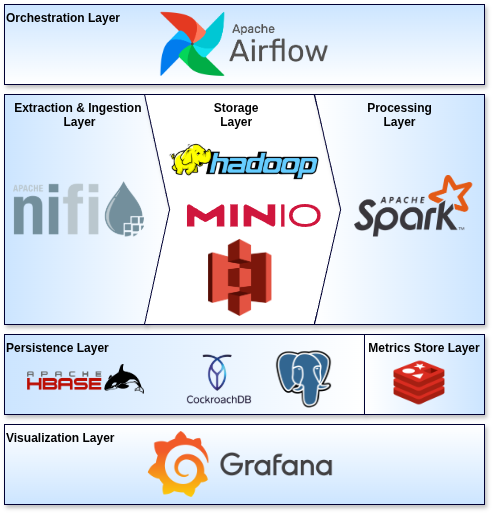
\includegraphics[width=0.45\textwidth]{../Report/graphs/BigDataStack}
    \caption{Big Data Stack di Sky Analytics Engine: rappresentazione dei livelli logici e delle tecnologie integrate.}
    \label{fig:big_data_stack}
\end{figure}

Il sistema evita l'approccio monolitico, configurandosi come un'aggregazione di servizi distribuiti coordinati che comunicano esclusivamente attraverso interfacce standardizzate.

% TODO: si può rimuovere per mettere il paragrafo su AI generativa
% L'infrastruttura è organizzata in macro-livelli gerarchici indipendenti, come illustrato nel Big Data Stack di riferimento (Fig.~\ref{fig:big_data_stack}).
% Questa netta separazione assicura che il sistema sia "future-proof": è possibile scalare o sostituire qualsiasi componente senza impattare gli altri livelli\@.

% I livelli principali sono:
% \begin{enumerate}
%     \item \textbf{Orchestration Layer:} Gestisce lo scheduling e lo stato delle esecuzioni.
%     \item \textbf{Extraction \& Ingestion Layer:} Si occupa dell'acquisizione sicura e della trasformazione dei dati.
%     \item \textbf{Storage Layer:} Funge da repository per i dati raw e pre-processati .
%     \item \textbf{Processing Layer:} Esegue il calcolo distribuito e l'addestramento dei modelli ML.
%     \item \textbf{Persistence Layer:} Implementa la persistenza multi-modello dei risultati.
%     \item \textbf{Metrics Store Layer:} Memorizza la telemetria di sistema.
%     \item \textbf{Visualization Layer:} Fornisce l'interfaccia di analisi visiva.
% \end{enumerate}

\subsection{Livello di Orchestrazione}\label{subsec:orchestration_layer}
In SAE, Apache Airflow non viene utilizzato per un singolo flusso lineare, ma gestisce una suite di tre DAG specializzati, ciascuno progettato per coprire un aspetto specifico del ciclo di vita del software e della validazione sperimentale\@.

\subsubsection{Disaccoppiamento tramite Apache Livy}
Una caratteristica architetturale di rilievo è l'integrazione di Apache Livy.
Nelle architetture legacy, Airflow necessita dell'installazione dei binari client di Spark e Hadoop sui propri nodi worker per lanciare i job tramite \texttt{spark-submit}.
SAE supera questa limitazione interagendo esclusivamente con l'API REST di Livy.
Airflow prepara un payload JSON contenente il path del JAR (precedentemente caricato su HDFS o S3) e gli argomenti di classe, inviandoli a Livy.
Questo approccio trasforma di fatto il cluster Spark in una risorsa "Compute-as-a-Service", riducendo il carico computazionale sul nodo orchestratore e migliorando la sicurezza isolando il piano di controllo dal piano dati\@.

\subsubsection{Sincronizzazione Asincrona con NiFi}
L'interazione tra Airflow e NiFi avviene tramite l'utilizzo di callback asincrono.
Airflow avvia il flusso NiFi tramite una chiamata HTTP POST, fornendo un JWT generato a runtime e un identificatore di variabile univoco.
Successivamente, Airflow entra in uno stato di \textit{Sensor Polling}, consumando risorse minime.
Quando NiFi completa l'ingestion, utilizza il JWT per autenticarsi contro le API REST di Airflow e aggiornare la variabile di stato, sbloccando il DAG e permettendo l'avvio della fase di processing\@.

\subsubsection{DAG di Orchestrazione e Benchmarking}
Ciascun workflow è ingegnerizzato per eseguire specifiche fasi del ciclo di vita del dato o per automatizzare le sessioni di validazione sperimentale:

\begin{itemize}
    \item[\textbf{1)}] \textbf{Workflow Principale:} Coordina l'interazione end-to-end tra il livello di ingestion e quello di calcolo.
    Al fine di massimizzare la flessibilità operativa, il DAG supporta la parametrizzazione a runtime, potendo utilizzare tre diverse modalità di esecuzione:
    \begin{itemize}
        \item \textit{Both:} Esegue la pipeline completa, dall'ingestion iniziale al processamento distribuito.
        \item \textit{Ingest Only:} Arresta il flusso subito dopo la conversione dei record in Parquet e il caricamento nel Data Lake.
        \item \textit{Execution Only:} Salta la fase di ingestion, avviando direttamente le classi analitiche di Spark sui dati Parquet preesistenti.
    \end{itemize}
    \vspace{0.1cm}

    \item[\textbf{2)}] \textbf{Benchmark Standalone:} Progettato specificamente per la raccolta sistematica dei dati di telemetria in ambienti locali o su istanze AWS EC2 standard.
    Al fine di garantire l'assoluta affidabilità dei benchmark analitici, questo DAG genera dinamicamente le task dependency tramite un costrutto ciclico in Python, forzando un'esecuzione puramente sequenziale di tutte le combinazioni possibili tra le query e i backend.
    Tale isolamento temporale impedisce la sovrapposizione computazionale e l'interferenza sull'I/O di rete o sul disco, restituendo metriche pulite.
    \vspace{0.1cm}

    \item[\textbf{3)}] \textbf{Benchmark Cloud-Native:} Sviluppato per automatizzare la valutazione sperimentale sull'infrastruttura fully-managed AWS EMR.
    Questo workflow bypassa il middleware Apache Livy e si interfaccia direttamente con i servizi infrastrutturali di Amazon Web Services sfruttando l'operatore \textit{EmrAddStepsOperator} per iniettare i job Java sotto forma di step sequenziali nel cluster e delegando il tracciamento allo stato di \textit{EmrStepSensor}.
    Questo design permette di sfruttare nativamente i meccanismi cloud AWS\@.
\end{itemize}

\subsection{Livello di Ingestion}\label{subsec:ingestion_layer}
Apache NiFi è la spina dorsale del livello di acquisizione dati.
La sua architettura basata sul paradigma Flow-Based Programming garantisce un controllo visivo e transazionale sui flussi di dati, garantendo anche la Data Provenance\@.

\subsubsection{Pipeline di Trasformazione}
Il flusso \texttt{SAE\_Ingestion\_Pipeline} implementa un processo articolato nelle seguenti fasi:
\begin{itemize}
    \item \textbf{Orchestrazione e Metadati:} Il processore \texttt{EvaluateJsonPath} estrae dal payload di trigger inviato da Apache Airflow le configurazioni dinamiche e i parametri di attivazione della pipeline.
    \item \textbf{Fetch, Validazione e Unzip:} Tramite \texttt{InvokeHTTP} viene effettuato il download del pacchetto compresso dal server sorgente.
    Un processore calcola l'hash SHA-1 confrontandolo con la firma attesa per garantirne l'integrità.
    Successivamente, il flusso esegue la decompressione dello zip, isolando i file CSV d'interesse e scartando i contenuti superflui.
    \item \textbf{Staging del Dato Grezzo:} I file CSV risultanti vengono immediatamente persistiti all'interno del Data Lake nella loro forma originaria, garantendo la presenza di uno storico del dato grezzo.
    \item \textbf{Normalizzazione e Conversione Colonnare:} Questa fase rappresenta il core computazionale del flusso.
    Attraverso il processore \texttt{ConvertRecord}, guidato da uno schema Avro fortemente tipizzato, NiFi preleva i CSV, ne normalizza la struttura e li converte nel formato colonnare Parquet.
    \item \textbf{Persistenza Finale e Notifica:} I file Parquet ottimizzati vengono salvati nello storage intermedio.
    Al completamento delle operazioni di scrittura, NiFi invia una notifica di successo ad Airflow per segnalare la terminazione della pipeline e consentire l'avanzamento dei DAG successivi.
\end{itemize}

\subsubsection{Formato dei Dati}
La scelta di convertire i dati nel formato colonnare Parquet costituisce il fondamento per massimizzare le performance.
Su questa base, il valore aggiunto del livello di ingestion è la capacità di NiFi di configurare dinamicamente a runtime la strategia di persistenza fisica dei file, in base ai parametri di orchestrazione ricevuti.
Il sistema permette infatti di selezionare due diverse tecniche per l'ottimizzazione dell'I/O in fase di lettura:
\begin{itemize}
    \item \textbf{Predicate Pushdown}: Sfrutta l'architettura nativa del formato Parquet, che include metadati statistici e dizionari a livello di singolo blocco.
    Il motore Catalyst di Spark utilizza queste informazioni per filtrare i dati direttamente in lettura, riducendo drasticamente il traffico di rete.
    \item \textbf{Partition Pruning}: Prevede la strutturazione fisica del Data Lake in directory gerarchiche basate sui valori di specifiche chiavi (anno, mese, carrier) dove NiFi instrada dinamicamente i record Parquet in base al contenuto.
    Durante l'esecuzione delle query, Spark valuta i filtri per escludere a priori la lettura di intere directory non rilevanti.
\end{itemize}

\subsubsection{Pre-processing e Data Quality}
La fase di ingestion non si limita alla mera conversione di formato, ma esegue un rigoroso controllo di qualità e pulizia del dato in streaming tramite processori NiFi dedicati.
I dati grezzi, infatti, possono presentare potenzialmente diverse inconsistenze, come valori di ritardo negativi sporchi, campi chiave mancanti e stati logici contraddittori.

La pipeline implementa due logiche fondamentali per garantire l'integrità analitica a valle:
\begin{itemize}
    \item \textbf{Normalizzazione e Gestione dei Ritardi:} Tramite script dedicati nel processore \texttt{ScriptedTransformRecord}, la pipeline neutralizza le componenti di ritardo negative e gestisce i valori mancanti delle singole cause.
    Nello specifico, se è presente almeno una causa di ritardo diversa da zero, i restanti valori nulli vengono sovrascritti a 0, altrimenti vengono lasciati invariati.
    \item \textbf{Filtraggio delle Inconsistenze Logiche:} Attraverso l'uso di query SQL sul processore \texttt{QueryRecord}, vengono scartati i record anomali che presentano discrepanze non recuperabili, quali: assenza di campi temporali o identificativi della compagnia, voli contrassegnati come cancellati ma recanti un orario di partenza effettivo, voli non cancellati ma privi di orario di arrivo/partenza, oppure evidenti errori matematici (es. ritardo totale negativo a fronte di una somma delle cause di ritardo positiva).
\end{itemize}

% impostiamo a NULL tutte le componenti di ritardo negative e a 0 quelle nulle con almeno una componente di ritardo positiva
% def delayFields = ["CARRIER_DELAY", "WEATHER_DELAY", "NAS_DELAY", "SECURITY_DELAY", "LATE_AIRCRAFT_DELAY"]
%
% // Check if there is at least one non-null delay cause
% boolean hasSignificantDelay = false
% delayFields.each { field ->
% def val = record.getValue(field)
% if (val != null) {
%     hasSignificantDelay = true
% }
% }
%
% // Apply the imputation logic
% if (hasSignificantDelay) {
%     // The flight has a significant delay: set null causes to 0 (they did not contribute)
%     // and fix any dirty negative values
%     delayFields.each { field ->
%     def val = record.getValue(field)
%     if (val == null) {
%         record.setValue(field, 0.0d)
%     } else if (((Number) val).doubleValue() < 0) {
%         record.setValue(field, 0.0d)
%     }
%     }
% }
% // If hasSignificantDelay is false, all fields are null and remain untouched.
%
% return record
%
%
% filtriamo i voli (e li cancelliamo) se hanno:
% - anno, mese, giorno, compagnia nulle
% - volo cancellato ma DEP_TIME non nullo
% - volo non cancellato ma DEP_TIME nullo O ARR_TIME nullo
% - volo con ARR_DELAY negativo ma somma dei componenti di ritardo positiva
%
% SELECT * FROM FLOWFILE
% WHERE "YEAR" IS NULL
%         OR "MONTH" IS NULL
%         OR DAY_OF_MONTH IS NULL
%         OR OP_UNIQUE_CARRIER IS NULL
%         OR (CANCELLED = 1.0 AND DEP_TIME IS NOT NULL)
%         OR (CANCELLED = 0.0 AND (DEP_TIME IS NULL OR ARR_TIME IS NULL))
%         OR ( (COALESCE(CARRIER_DELAY, 0.0) + COALESCE(WEATHER_DELAY, 0.0) + COALESCE(NAS_DELAY, 0.0) + COALESCE(SECURITY_DELAY, 0.0) + COALESCE(LATE_AIRCRAFT_DELAY, 0.0)) > 0.0 AND ARR_DELAY < 0.0 )

\subsection{Livello di Storage}\label{subsec:storage_layer_datalake}
Il cuore della persistenza intermedia è rappresentato dal Data Lake, implementato tramite Hadoop HDFS o MinIO in ambienti on-premise e Amazon S3 in configurazioni cloud.
Questo strato funge da \textit{Single Source of Truth}, sfruttando la capacità intrinseca dello storage di accogliere e centralizzare dati eterogenei.
% senza la necessità di un pre-processing o di uno schema rigido preventivo.

L'infrastruttura ospita sia i dataset grezzi originari acquisiti da NiFi, sia i dati successivamente raffinati e convertiti in formato Parquet.
Nelle distribuzioni cloud basate su Amazon S3, questa architettura abilita un disaccoppiamento totale tra le risorse di storage e quelle di calcolo, garantendo una scalabilità indipendente.
% Inoltre, la strutturazione dei dati raffinati in formato Parquet permette a Spark di eseguire ottimizzazioni avanzate, come il \textit{predicate pushdown} e la \textit{column projection}, riducendo drasticamente l'I/O complessivo durante le fasi di analisi.

\subsection{Livello di Processing}\label{subsec:processing_layer}
Il cuore computazionale di SAE è l'applicazione Spark.

% La modularità del codice sorgente è stata ottenuta applicando rigorosamente i design pattern della programmazione orientata agli oggetti\@.

\subsubsection{Pattern Factory e Repository}
Per astrarre l'accesso ai dati, SAE implementa il pattern Repository.
L'interfaccia \texttt{FlightRepository} definisce metodi generici come \texttt{getFlights()} e \texttt{saveResults()}.
Tramite la classe \texttt{FlightRepositoryFactory}, l'applicazione istanzia a runtime implementazioni specifiche basandosi su un file di configurazione YAML, gestito attraverso la classe \texttt{ApplicationConfig}.
Questo significa che la logica di business analitica è completamente disaccoppiata dalla tecnologia di storage sottostante\@.

\subsubsection{Astrazione delle Query}
Ogni query estende la classe astratta \texttt{BaseQuery}.
Questa classe si fa carico del boilerplate code: istanziazione della \texttt{SparkSession}, gestione del logging strutturato, iniezione del listener delle metriche e recupero dei dati dal repository.
Le classi figlie devono implementare esclusivamente tre metodi: \texttt{runQueryRDD}, \texttt{runQueryDataFrame} e \texttt{runQuerySQL}, focalizzandosi solo sulla trasformazione del dato\@.

\subsubsection{Test di Coerenza}
L'architettura garantisce l'integrità del calcolo attraverso una suite di test di coerenza locale.
Questi test caricano il dataset Parquet reale fornito e verificano che i risultati ottenuti tramite le tre diverse astrazioni di Spark siano matematicamente equivalenti entro tolleranze definite (necessarie per gli algoritmi di sketching), assicurando che la logica di business sia preservata indipendentemente dal backend scelto\@.

\subsection{Livello di Persistenza}\label{subsec:persistence_layer}
Al fine di garantire massima flessibilità e supportare diverse strategie di storage per il serving dei risultati, SAE è progettato per integrarsi, in modo mutuamente esclusivo a seconda del deployment, con tre diversi motori di database:

\begin{itemize}
    \item \textbf{CockroachDB:} Rappresenta la scelta principale per ambienti di produzione distribuiti.
    Grazie alla sua architettura cloud-native e alla compatibilità con il protocollo PostgreSQL, offre scalabilità orizzontale e consistenza distribuita, mantenendo un'interfaccia SQL standard per l'integrazione nativa con strumenti come Grafana.
    \item \textbf{PostgreSQL:} Utilizzato come alternativa lightweight a CockroachDB per deployment standalone, testing o ambienti di sviluppo locale, mantenendo invariata la logica di accesso ai dati SQL.
    \item \textbf{Apache HBase:} Implementa il paradigma NoSQL a colonne larghe ed è configurabile come alternativa ai database relazionali qualora sia necessario memorizzare dataset di risultati estremamente granulari, garantendo tempi di accesso nell'ordine dei millisecondi per singole chiavi su volumi massivi.
\end{itemize}

\subsection{Metrics Store Layer}\label{subsec:metrics_store_layer}
Redis Stack è il componente dedicato esclusivamente alla memorizzazione della telemetria applicativa emessa in tempo reale. 
Per alimentare questo layer, SAE implementa la classe \texttt{JobTimerListener}, che estende le interfacce native dello \texttt{SparkListener} e viene agganciata al bus degli eventi di Spark durante l'inizializzazione della sessione.

Il Listener intercetta eventi cruciali (come \texttt{onJobStart}, \texttt{onStageCompleted} e \texttt{onTaskEnd}), registrando metriche relative alle tempistiche impiegate e al volume di dati letti e scritti.
Alla fine del ciclo di vita dell'applicazione, il sistema aggrega questi dati e, sfruttando Redis, persiste i record di telemetria.
Questo approccio permette di scorporare il "vero" tempo di calcolo sui dati dal tempo fisiologico speso da Spark per negoziare le risorse con il manager, garantendo un'analisi dei benchmark estremamente accurata.

\subsection{Visualization Layer}\label{subsec:visualization_layer}
Grafana rappresenta il punto di accesso finale per l'analisi visiva dei dati. 
Configurato per interrogare sia CockroachDB (per i risultati di business) che Redis (per la telemetria tecnica tramit RediSearch), il sistema fornisce dashboard interattive progettate per presentare in un unico ambiente le performance infrastrutturali con gli insight analitici estratti.

% \begin{itemize}
%     \item Benchmark prestazionali comparativi basati sulla telemetria distribuita.
%     \item Trend temporali dei ritardi suddivisi per vettore.
%     \item Andamento della distribuzione oraria calcolata sui percentili approssimati.
%     \item La disposizione geometrica dei cluster ML nello spazio delle feature principali.
% \end{itemize}

% Tale integrazione permette di correlare in un unico ambiente le performance infrastrutturali con gli insight analitici estratti dalla pipeline.

% ------------------------------

\section{Implementazioni delle Analisi Distribuite}\label{sec:implementation_details}
Le quattro query richieste sono state implementate in modo da testare diverse astrazioni di Spark e valutare i trade-off tra controllo a basso livello ed engine ottimizzati.

\subsection{Query 1: Statistiche Mensili}
La \textit{Query 1} richiede il calcolo di statistiche mensili (media, min, max, tasso di cancellazione) per specifiche compagnie.
La struttura logica dell'esecuzione è visualizzabile nel DAG di Spark riportato in Appendice~\ref{sec:appendix_spark_dags} (Fig.~\ref{fig:dag_q1}).

L'implementazione basata su RDD si articola nelle seguenti fasi:
\begin{itemize}
    \item \textbf{Map-Side Aggregation con \texttt{aggregateByKey}:} Si è evitato l'uso dell'operatore \texttt{groupByKey}, un'operazione che può causare colli di bottiglia prestazionali a causa del trasferimento di dati sulla rete durante la fase di \textit{shuffle}.
    Al suo posto è stato utilizzato \texttt{aggregateByKey}, il quale combina i valori parzialmente all'interno di ogni singola partizione del nodo worker prima di trasferirli sulla rete tramite combiner, riducendo drasticamente il volume di dati movimentato nello shuffle.
    \item \textbf{Struttura dell'Accumulatore:} Viene impiegato un array di \texttt{double} come accumulatore compatto per ogni chiave \texttt{(Carrier, Month)}:
    \[
    \mathcal{A}_{Q1} = \langle \textstyle \sum D_{dep}, \max(D_{dep}), \min(D_{dep}), N_{vld}, N_{tot} \rangle
    \]
    dove $D_{dep}$ è il ritardo, $N_{vld}$ i voli non cancellati e $N_{tot}$ i totali.
    \item \textbf{Trasformazione Finale:} Un'operazione di \texttt{map} elabora i valori dell'accumulatore per calcolare le medie definitive ($ \sum D_{dep} / N_{valid} $) e i tassi di cancellazione ($ (N_{tot} - N_{valid}) / N_{tot} $), restituendo il formato finale richiesto per la persistenza.
\end{itemize}

\subsection{Query 2: Decomposizione dei Ritardi}\label{subsec:query2_details}
La \textit{Query 2} analizza la composizione dei ritardi e richiede logiche di \textit{feature engineering} per gestire correttamente i dati sparsi.
Una peculiarità del dominio applicativo riguarda la dichiarazione delle cause di ritardo: per legge federale, le compagnie aeree non sono tenute a specificare i motivi dettagliati se il ritardo complessivo all'arrivo è inferiore ai 15 minuti.
Questa condizione genera una significativa presenza di valori mancanti nel dataset.

Al fine di rispondere correttamente al requisito di calcolare il \textbf{contributo medio} delle diverse cause di ritardo, viene implementata una strategia di imputazione a zero per i valori mancanti (utilizzando l'operatore \texttt{coalesce} in Spark e pre-elaborando i record parziali in NiFi).
Questa scelta metodologica è fondamentale per distinguere tra due possibili approcci analitici:
\begin{itemize}
    \item \textbf{Analisi dell'Intensità:} Ignorando i valori nulli, il calcolo della media includerebbe solo i voli con ritardo conclamato.
    Sebbene utile per misurare la severità di un problema quando si verifica, questo approccio distorcerebbe la visione d'insieme, sovrastimando l'impatto delle singole cause sull'operatività totale.
    \item \textbf{Analisi del Contributo Medio :} Trattando i valori mancanti come zero, il denominatore della media è costituito dalla totalità dei voli non cancellati e non deviati della compagnia.
    In questo modo, il risultato esprime quanto mediamente ogni causa pesi su tutto il dataset dei voli considerati.
\end{itemize}

Tale approccio fornisce una visione realistica della resilienza del business, permettendo di identificare quali compagnie riescano effettivamente a mitigare l'impatto di specifiche cause su scala globale, anziché focalizzarsi esclusivamente sui casi limite.

Il piano di esecuzione distribuito è composto da tre job sequenziali (Fig.~\ref{fig:dag_q2} in Appendice~\ref{sec:appendix_spark_dags}).
L'implementazione basata su RDD si sviluppa come segue:
\begin{itemize}
    \item \textbf{Filtraggio Iniziale:} Un'operazione di \texttt{filter} scarta a priori i voli deviati o cancellati per garantire l'integrità del calcolo delle medie.
    \item \textbf{Map-Side Aggregation con \texttt{aggregateByKey}:} Similmente alla Query 1, viene utilizzato un accumulatore compatto associato alla chiave \texttt{Carrier}:
    \[
    \begin{aligned}
    \mathcal{A}_{Q2} = \langle N, \textstyle \sum D_{arr}, \textstyle \sum D_{carr}, \textstyle \sum D_{weat}, \\
    \textstyle \sum D_{nas}, \textstyle \sum D_{sec}, \textstyle \sum D_{late} \rangle
    \end{aligned}
    \]
    dove $N$ è il numero totale dei voli validi per il vettore e le successive componenti rappresentano le somme dei ritardi.
    \item \textbf{Filtro di Confidenza e Medie:} Una successiva operazione di \texttt{filter} mantiene solo le chiavi con $N \ge 500$. L'operazione di \texttt{map} calcola i contributi medi dividendo le somme parziali per $N$.
    \item \textbf{Ranking Globale:} Un \texttt{sortBy} distribuito sulle medie, seguito da \texttt{zipWithIndex} e \texttt{filter}, permette di estrarre la top 10 dei vettori. L'ordinamento globale in questa fase non costituisce un bottleneck poiché i dati in shuffle sono ormai collassati a un singolo record per compagnia aerea validata.
\end{itemize}

\subsection{Query 3: Percentili per Fasce Orarie}
Il calcolo dei percentili su finestre orarie nella \textit{Query 3} rappresenta la sfida computazionale più ardua.
Un calcolo esatto richiederebbe l'ordinamento globale di milioni di record, un'operazione che su un cluster distribuito causa enormi colli di bottiglia dovuti allo scambio di dati.

SAE risolve questo problema implementando tecniche di "Quantile Sketching".
Attraverso l'integrazione della libreria Apache DataSketches, è stato implementato lo stimatore Karnin-Lang-Liberty.
Parallelamente, per offrire una maggiore flessibilità analitica, il sistema integra anche l'algoritmo T-Digest.
Entrambi gli stimatori sono configurabili a runtime tramite la proprietà \texttt{percentileAlgorithm} in \texttt{ApplicationConfig}.

L'algoritmo KLL, in particolare, mantiene in memoria un set compresso e rappresentativo dei dati osservati.
La potenza matematica di questi algoritmi di sketching risiede nella loro proprietà di unione: due sketch generati su nodi worker differenti possono essere sommati nel driver node mantenendo rigorose garanzie matematiche sull'errore di rango massimo (configurato di default a $\sim 1.6\%$ per KLL).
Questo permette di calcolare i percentili orari in un singolo passaggio sui dati, con una complessità spaziale fissa indipendente dalla dimensione del dataset.
La complessità del piano fisico è riflessa nei due job Spark visibili in Fig.~\ref{fig:dag_q3} (Appendice~\ref{sec:appendix_spark_dags}).

Nell'implementazione specifica RDD, la query si divide in due pipeline parallele:
\begin{itemize}
    \item \textbf{Pipeline dei Percentili:} Sfrutta l'operatore \texttt{combineByKey} per gestire l'istanziazione, l'aggiornamento e l'unione dei buffer binari che rappresentano lo stato interno dello sketch scelto (KLL o T-Digest). La struttura dati scambiata durante la \textit{combine} è:
    \[
    \mathcal{S}_{Q3} = \langle byte[] \text{ (Sketch State Buffer)} \rangle
    \]
    Questo buffer compatto riduce l'I/O ed è associato alla chiave composita \texttt{(Carrier, Hour)}.
    \item \textbf{Pipeline Globale:} Opera parallelamente per calcolare i valori estremi per ogni \texttt{Carrier}. Utilizza \texttt{aggregateByKey} con un accumulatore di dimensione fissa:
    \[
    \mathcal{A}_{Q3} = \langle \min(D_{dep}),\; \max(D_{dep}) \rangle
    \]
\end{itemize}
Entrambe le pipeline agiscono su un RDD preventivamente filtrato e cachato in memoria per evitare la rilettura ripetuta dei medesimi record dal livello di storage.

Nell'implementazione DataFrame, il sistema delega questa approssimazione alla funzione nativa \texttt{percentile\_approx}, la quale utilizza un approccio simile derivato dall'algoritmo Greenwald-Khanna.

\subsection{Query 4: Clustering delle Compagnie}
L'obiettivo della \textit{Query 4} è raggruppare le compagnie aeree in base alle loro feature prestazionali.

A differenza delle analisi precedenti, questa query è implementata unicamente tramite le API DataFrame.
Il framework di machine learning di Spark, e in particolare le sue funzionalità di \textit{feature extraction} e le implementazioni ottimizzate del K-Means, dipendono strutturalmente dall'astrazione \texttt{Dataset<Row>} e dai tipi \texttt{Vector}.
Riscrivere il processo utilizzando le API RDD sottostanti annullerebbe i benefici di tali ottimizzazioni ed esporrebbe ad operazioni scalari inefficienti.

L'implementazione in \texttt{AirlineClustering} costruisce una complessa pipeline:
\begin{enumerate}
    \item \textbf{Aggregazione Iniziale:} Calcolo delle feature medie per carrier escludendo i voli cancellati dai conteggi di ritardo.
    \item \textbf{Vector Assembler:} Consolidamento delle colonne numeriche in una singola colonna di tipo \texttt{Vector}, formato richiesto da MLlib.
    \item \textbf{Standardization:} Applicazione di uno \texttt{StandardScaler}.
    Poiché il k-Means è sensibile alla scala delle feature (basandosi sulla distanza euclidea), è imperativo normalizzare i dati affinché abbiano media 0 e deviazione standard 1, evitando che feature con magnitudo maggiore dominino l'algoritmo.
    \item \textbf{Cluster Number Selection:} Il sistema non richiede di specificare a priori il parametro $K$, ovvero il numero di cluster.
    Il sistema esegue un loop iterativo addestrando modelli da $K=2$ a $K=5$.
    Per ogni modello, valuta la qualità del raggruppamento utilizzando il \textit{Silhouette Score}.
    Il punteggio di Silhouette misura la coesione intra-cluster rispetto alla separazione inter-cluster.
    SAE seleziona dinamicamente il $K$ che massimizza questo punteggio, garantendo un clustering statisticamente fondato.
\end{enumerate}

% ------------------------------

\section{Infrastruttura di Deployment}\label{sec:deployment_infrastructure}
L'agilità di SAE è esaltata dalle sue procedure di deployment, strutturate in due macro-scenari.
L'esternalizzazione della configurazione in file YAML e \texttt{.env} evita l'uso di stringhe di connessione o path assoluti hardcoded, grazie a cui è possibile compilare il JAR una sola volta tramite Maven ed eseguirlo in contesti completamente diversi.

\subsection{Ambiente Standalone AWS EC2}
Il primo macro-scenario simula un'infrastruttura di tipo locale o on-premise virtualizzata in cloud.

\begin{figure}[!htbp]
    \centering
    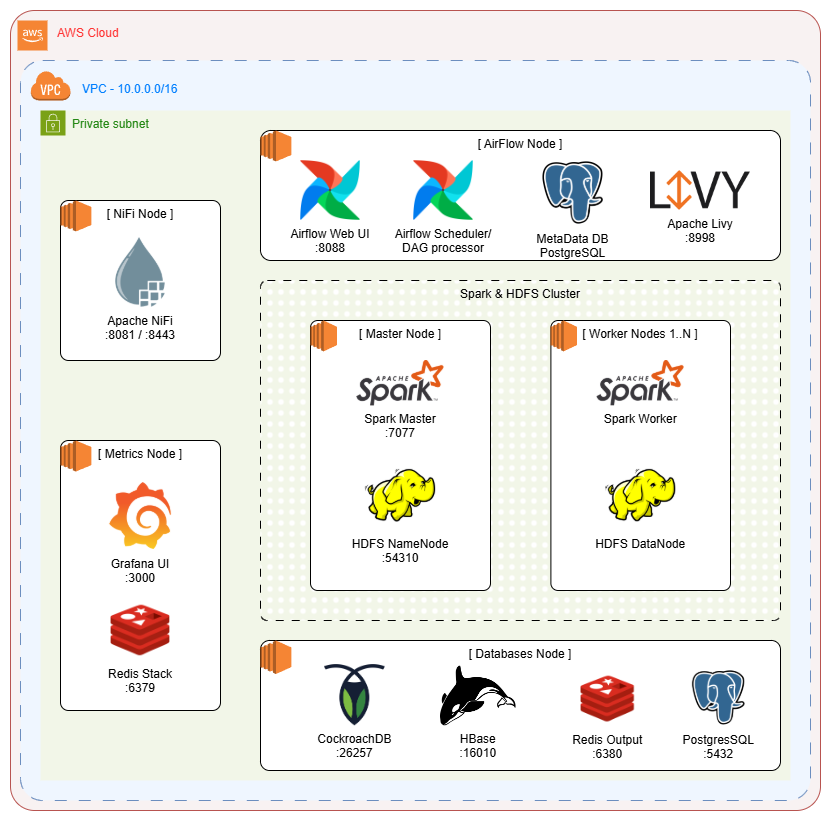
\includegraphics[width=0.47\textwidth]{../Report/graphs/DeploymentView-EC2}
    \caption{Diagramma di deployment di Sky Analytics Engine su AWS EC2: rappresentazione dei componenti distribuiti.}
    \label{fig:deployment_bigdata_diagrams}
\end{figure}

Il deployment si avvale di una suite di istanze Amazon EC2 attestate all'interno della medesima Virtual Private Cloud (Fig.~\ref{fig:deployment_bigdata_diagrams}):

\begin{itemize}
    \item \textbf{Airflow Node (1x \texttt{t3.medium}):} Nodo di controllo primario che ospita l'interfaccia Web di Airflow, lo Scheduler, il database dei metadati e il middleware Apache Livy.
    \item \textbf{NiFi Node (1x \texttt{t3.small}):} Dedicato esclusivamente all'esecuzione di Apache NiFi per l'ingestion e la trasformazione colonnare.
    \item \textbf{Metrics Node (1x \texttt{t3.small}):} Ospita lo stack di monitoraggio, composto da Grafana e Redis Stack per la telemetria.
    \item \textbf{Databases Node (1x \texttt{t3.small}):} Centralizza i motori di persistenza dei risultati, inclusi CockroachDB, Apache HBase e PostgreSQL.
    \item \textbf{Spark \& HDFS Cluster:} 
    \begin{itemize}
        \item \textbf{Master Node (1x \texttt{t3.small}):} Esegue lo Spark Master e l'HDFS NameNode.
        \item \textbf{Worker Nodes (Nx \texttt{t3.small}):} Nodi di calcolo e storage che ospitano gli Spark Worker e gli HDFS DataNode.
    \end{itemize}
\end{itemize}
In questa configurazione, HDFS funge da file system distribuito primario, mentre la sottomissione dei job Spark avviene in modalità client tramite Apache Livy, garantendo il completo disaccoppiamento logico ed architetturale\@.

\subsection{Ambiente Cloud-Native AWS EMR}
Il secondo scenario proietta SAE in una dimensione pienamente elastica ed enterprise-ready, sfruttando il servizio gestito Amazon Elastic MapReduce.
L'infrastruttura è configurata come segue:
\begin{itemize}
    \item \textbf{Master Node (1x \texttt{m6g.xlarge}):} Coordina il resource manager Hadoop YARN.
    \item \textbf{Core Nodes (3x \texttt{m6g.xlarge}):} Eseguono i demoni executor di Spark sotto il controllo di YARN e memorizzano i dati intermedi.
\end{itemize}
Il vantaggio cardine di questo scenario risiede nell'integrazione nativa dello storage con Amazon S3 mediante il protocollo \texttt{s3a://}.
Questo abilita un paradigma \textbf{Shared-Nothing} puro, in cui le risorse di calcolo possono essere scalate o spente in modo del tutto indipendente dallo storage persistente, azzerando i costi di idle e ottimizzando il total cost of ownership\@.

% ------------------------------

\section{Valutazione Sperimentale}\label{sec:experimental_evaluation}
Definita l'architettura e implementati i componenti, è stata condotta una fase di validazione sperimentale sistematica per valutare la robustezza, la scalabilità e le performance del sistema.
I test sono stati orchestrati in modo sequenziale tramite il DAG \texttt{ec2\_benchmark} su EC2 e \texttt{emr\_benchmark} su EMR, garantendo l'assenza di interferenze computazionali e l'affidabilità della telemetria raccolta.

\subsection{Analisi Comparativa delle Performance}\label{subsec:performance_analysis}
Le misurazioni prestazionali raccolte evidenziano trend marcati circa l'efficacia dei diversi backend di Apache Spark e l'impatto dell'infrastruttura di deployment.

\subsubsection{Dispersione Statistica dei Backend}
L'osservazione dei box plot in Appendice~\ref{sec:appendix_telemetry} rivela un comportamento dei backend computazionali strettamente legato non solo alla natura algoritmica della query, ma anche all'infrastruttura di esecuzione.

Negli scenari di aggregazione massiva e ordinamento (Query 1 e Query 2), indipendentemente dall'ambiente di esecuzione, le API strutturate presentano mediane prestazionali generalmente inferiori rispetto all'approccio RDD e mostrano una dispersione statistica decisamente più contratta.
Questa notevole stabilità prestazionale è una conseguenza diretta delle ottimizzazioni logiche del \textit{Catalyst Optimizer}.

L'analisi delle metriche introduce tuttavia un'interessante divergenza infrastrutturale nella Query 3.
In ambiente standalone su AWS EC2 (osservando la strategia Partition Pruning), l'approccio RDD fa registrare un'eccezione: una mediana del tempo di calcolo inferiore ($\sim 15s$ contro i $\sim 20s$ dei backend strutturati) e un box plot più compatto.
Questo comportamento su EC2 è riconducibile al minor overhead di astrazione dell'API RDD per computazioni non lineari: l'uso esplicito dell'operatore \texttt{combineByKey} applicato all'algoritmo KLL risulta localmente più efficiente del piano generato da Catalyst per la funzione \texttt{percentile\_approx}.

Il paradigma si ribalta radicalmente traslando l'esecuzione sull'ambiente managed AWS EMR. In questo contesto, il vantaggio dell'API RDD per la Query 3 viene completamente azzerato: DataFrame riprende il primato prestazionale ($\sim 7.8s$ contro gli $\sim 8.7s$ di RDD in Partition Pruning con KLL) ed esibisce una dispersione statistica minima.
% Questo scarto evidenzia l'impatto delle ottimizzazioni proprietarie dell'EMR Runtime per Apache Spark: l'engine managed di AWS è in grado di parallelizzare ed eseguire il piano logico di Catalyst con un'efficienza tale da superare le logiche custom RDD, penalizzando al contempo quest'ultimo a causa dei massicci volumi di Shuffle Read/Write indotti dalla serializzazione degli oggetti Java.

\subsubsection{Impatto dell'Infrastruttura sul Wall Clock Time}
Un aspetto cruciale che emerge dall'analisi comparativa è l'impatto dell'infrastruttura sul cosiddetto \textbf{Wall Clock Time}.
Come evidenziato dalla telemetria (Appendice~\ref{sec:appendix_telemetry}), il tempo totale misurato dal Driver Spark all'interno della fase di esecuzione è sistematicamente superiore al tempo puro di calcolo distribuito.

Questo overhead è generato da operazioni svolte localmente dalla JVM del Driver, al di fuori del ciclo di vita dei Job Spark, tra cui:
\begin{itemize}
    \item \textbf{Ottimizzazione Lazy:} Il tempo speso dal Driver per risolvere il piano logico, applicare le regole di ottimizzazione e compilare il piano fisico prima dell'effettiva sottomissione dei task.
    \item \textbf{I/O Setup e Validazione:} L'interazione con il \textit{NameNode} per HDFS o le API REST di Amazon S3 per la risoluzione dei path.
    \item \textbf{Consolidamento dell'Output:} Il tempo speso dal Driver al termine del job per rinominare e spostare i file temporanei generati dagli executor nelle directory di destinazione finali.
\end{itemize}

L'infrastruttura sottostante e il target di persistenza giocano un ruolo determinante nel giustificare questo scarto temporale.
Il confronto evidenzia come AWS EMR riesca a contrarre sensibilmente la quota di overhead rispetto al cluster standalone EC2.
Nel deployment su EC2, il consolidamento finale dei risultati prevede la scrittura su un database.
Questo approccio introduce latenze fisiologiche intrinseche: l'apertura e la gestione delle connessioni di rete da parte degli executor, la traduzione dei record e i tempi di attesa per il commit transazionale del motore di database.
Al contrario, l'ambiente AWS EMR abbatte questi tempi morti sfruttando l'integrazione nativa e ottimizzata per la persistenza diretta tramite S3, mitigando drasticamente il costo architetturale dell'I/O in fase di salvataggio.

\subsubsection{Confronto sulle Tecniche di Ottimizzazione dell'I/O}
Un'analisi fondamentale condotta in questa fase riguarda il confronto tra le due principali strategie di ottimizzazione dell'I/O: \textbf{Partition Pruning} e \textbf{Predicate Pushdown}.

L'osservazione dei tempi di esecuzione globali evidenzia come, a parità di query e di motore computazionale, le due tecniche garantiscano un tempo di calcolo complessivo molto simile.
Tuttavia, un'indagine approfondita della telemetria di basso livello rivela differenze architetturali radicali, in particolare per quanto concerne i volumi di I/O e la distribuzione della pressione computazionale sui nodi worker.

Il \textbf{Partition Pruning} si dimostra l'approccio nettamente più efficiente dal punto di vista infrastrutturale.
Escludendo a priori le partizioni non necessarie a livello di file system, Spark evita del tutto l'apertura e la scansione dei file irrilevanti.
Questo si traduce in un sensibile abbattimento dei byte complessivamente letti e, fattore ancora più critico, in un'ottimale ripartizione del lavoro tra i worker.
L'analisi della metrica \textit{Executor Workload Skewness} dimostra infatti che, con l'utilizzo del pruning, il volume medio di dati assegnato ai nodi si sovrappone in modo quasi perfetto al picco massimo elaborato dal singolo esecutore.
Questo parallelismo ben bilanciato garantisce l'assenza di colli di bottiglia e un utilizzo omogeneo delle risorse.

Al contrario, il \textbf{Predicate Pushdown} impone a Spark l'accesso sistematico ai metadati interni dei file Parquet per valutarne le statistiche prima del filtraggio.
Sebbene questa tecnica si confermi efficace nel ridurre i record effettivamente passati alle fasi successive della pipeline, essa genera un volume di lettura fisicamente molto più elevato sull'infrastruttura di storage e introduce un grave sbilanciamento del carico.
Come evidenziato in modo inequivocabile dalla telemetria, il picco massimo di byte letti risulta essere esattamente il triplo della media teorica.
Considerando l'architettura a tre nodi worker del cluster, questo dato dimostra che le dinamiche di partizionamento dei task portano un singolo esecutore a farsi carico del 100\% della scansione iniziale, lasciando gli altri inattivi e trasformando il nodo in un temporaneo collo di bottiglia.

Questo divario nell'efficienza di lettura e nel bilanciamento dei task è particolarmente palese nell'analisi dei percentili orari, dove il Partition Pruning riesce a contenere l'I/O overhead garantendo al contempo una sottomissione dei task lineare ed equa sui nodi, mitigando lo stress infrastrutturale in modo speculare sia in ambiente standalone AWS EC2 che nella controparte elastica AWS EMR\@.

\subsection{Discussione dei Risultati Analitici}\label{subsec:analytical_results_discussion}

L'obiettivo di questa fase non è fornire un'indagine esaustiva sul dominio aeronautico, bensì validare le capacità analitiche della piattaforma SAE su un dataset reale, dimostrando come riesca a estrarre pattern operativi coerenti.

\subsubsection{Query 1: Performance Mensili delle Compagnie}
L'analisi del quadrimestre evidenzia comportamenti diametralmente opposti tra American Airlines (AA) e Delta Air Lines (DL) (Fig.~\ref{fig:results_q1_average_delay_trend} in Appendice~\ref{sec:appendix_results}). A gennaio entrambe registrano il proprio picco di cancellazioni (AA: $3,65\%$, DL: $2,67\%$), ma nei mesi successivi le efficienze divergono:
\begin{itemize}
    \item \textbf{Delta Air Lines:} Mostra un miglioramento costante.
    Il ritardo medio alla partenza scende da $12,8$ minuti a gennaio fino a $8,7$ minuti ad aprile, con un tasso di cancellazioni che si stabilizza sotto lo $0,50\%$.
    \item \textbf{American Airlines:} Subisce un degrado progressivo.
    Il ritardo medio sale da $12,9$ a $16,0$ minuti, mantenendo un tasso di cancellazione fisso e più elevato, attorno all'$1,40\%$.
\end{itemize}

\subsubsection{Query 2: Decomposizione delle Cause di Ritardo}
La classifica dei top 10 vettori per ritardo all'arrivo (Fig.~\ref{fig:results_q2_top10_arrival_delay} in Appendice~\ref{sec:appendix_results}) evidenzia dinamiche strutturali diverse.
\textbf{PSA Airlines (OH)} risulta in assoluto più inefficiente ($17,16$ minuti di ritardo medio), penalizzato in modo massiccio dal \textit{late aircraft delay}.
Questo indica una forte incapacità di assorbire i ritardi pregressi, che finiscono per propagarsi a cascata sui voli successivi.
Al contrario, \textbf{United Airlines (UA)} mantiene il ritardo all'arrivo più basso ($2,46$ minuti) e un'ottima gestione interna, ma subisce il forte impatto del \textit{NAS delay} (ritardi legati al controllo del traffico aereo), a dimostrazione di una maggiore esposizione alla congestione fisiologica degli scali.

\subsubsection{Query 3: Distribuzione Oraria dei Percentili di Ritardo}
L'analisi oraria (riportata in Appendice~\ref{sec:appendix_results}) conferma un deterioramento fisiologico delle performance con il passare delle ore, ma con impatti molto diversi tra le compagnie.
Il 90° percentile di American Airlines, ad esempio, arriva fino ai $70$ minuti nella fascia serale, evidenziando una severa incapacità di smaltire la congestione diurna.
Delta Air Lines, di contro, mantiene una curva di crescita più dolce e controllata.

Un aspetto metodologico cruciale per SAE emerge dal confronto diretto degli algoritmi nei grafici risultanti: Il confronto sperimentale tra gli algoritmi all'interno del contesto SAE ha confermato le aspettative teoriche, evidenziando un netto trade-off tra memoria e potenza di calcolo senza decretare un vincitore assoluto. Da un lato, l'algoritmo KLL richiede un maggiore impiego di memoria per preservare la sua struttura a piramide dei livelli, un costo spaziale chiaramente visibile nei grafici di shuffle read. Dall'altro lato, il T-Digest risulta più efficiente in termini di spazio, poiché memorizza solo i centroidi, ma sconta una maggiore lentezza computazionale dovuta ai calcoli continui della funzione di scala necessari per l'aggiornamento dei cluster stessi. Siccome i risultati analitici di entrambe le euristiche sono molto simili, la scelta tra i due metodi dipende quindi dai vincoli infrastrutturali a disposizione (Appendice~\ref{sec:appendix_spark_dags}).
\subsubsection{Query 4: Clustering delle Compagnie Aeree}
L'applicazione dell'algoritmo K-Means con selezione automatica del modello tramite Silhouette Score ha identificato $K=3$ come il numero ottimale di raggruppamenti statistici per descrivere le compagnie (Fig.~\ref{fig:results_q4_cluster_distribution} in Appendice~\ref{sec:appendix_results}).
Per scopi di visualizzazione bidimensionale, è stata utilizzata una \textbf{Principal Component Analysis} per proiettare i centroidi e l'appartenenza dei vettori (Fig.~\ref{fig:results_q4_cluster_distribution}). Tuttavia, è fondamentale sottolineare che tale proiezione spaziale a due sole componenti principali offre una rappresentazione semplificata e parzialmente approssimata, comportando una fisiologica perdita di precisione.
L'algoritmo di clustering, al contrario, ha operato addestrandosi sull'intero spazio ad alta dimensionalità delle feature originali.

L'analisi congiunta di questa proiezione e della matrice di classificazione (i cui valori medi normalizzati per cluster sono riportati in Fig.~\ref{fig:results_q4_cluster_center} in Appendice~\ref{sec:appendix_results}, mentre la Tabella~\ref{tab:results_q4_metrics} ne riporta i corrispondenti valori operativi reali) delinea tre cluster operativi ben definiti:

\begin{itemize}
    \item \textbf{Cluster 0 - Inefficienza Operativa e Propagazione:} È il raggruppamento che presenta le criticità maggiori.
    Vettori come \texttt{OH} e \texttt{F9} guidano il cluster con ritardi all'arrivo elevatissimi, causati da un forte effetto di propagazione a catena.
    Nel caso estremo di \texttt{OH}, l'instabilità si traduce anche in un tasso di cancellazione critico, superiore al $6\%$.
    \item \textbf{Cluster 1 - Sensibilità Esterna:} Formato unicamente da \textbf{Allegiant Air (\texttt{G4})}.
    Questa compagnia delinea un profilo anomalo: subisce forti ritardi in partenza a causa di fattori esterni incontrollabili (ritardi meteorologici e di sicurezza).
    Tuttavia, registra un tasso di cancellazioni bassissimo ($0,6\%$), denotando una politica aziendale orientata a completare i voli programmati indipendentemente dalle avversità e dai ritardi accumulati.
    \item \textbf{Cluster 2 - Alta Efficienza e Stabilità:} È il gruppo nettamente più virtuoso.
    Questi vettori gestiscono il traffico con estrema regolarità, mostrando ritardi all'arrivo minimi (\texttt{YX} scende addirittura a una media di $0,69$ minuti) e una notevole flessibilità di rete.
    La loro caratteristica chiave è l'eccellente capacità di recuperare tempo in volo, evidenziata da valori di \textit{delay makeup} nettamente negativi, che in molti casi permettono di recuperare oltre $6$ minuti rispetto alla schedulazione originaria.
\end{itemize}

% ------------------------------

\section{Conclusioni e Sviluppi Futuri}\label{sec:conclusions_future_work}
Sky Analytics Engine dimostra che l'implementazione rigorosa di pattern architetturali distribuiti e l'adozione strategica di formati dati ottimizzati rappresentano requisiti imprescindibili per dominare la complessità inerente ai Big Data.
L'orchestrazione asincrona tra Apache Airflow e NiFi, combinata con la modularità dell'engine Spark, ha permesso di costruire un ecosistema robusto, scalabile ed enterprise-ready.

I risultati sperimentali hanno validato le scelte ingegneristiche effettuate.
L'utilizzo combinato del formato colonnare Parquet e delle tecniche di Partition Pruning ha consentito di abbattere l'I/O overhead sul file system distribuito.
Inoltre, l'integrazione di tecniche algoritmiche, quali gli stimatori probabilistici Quantile Sketches e il Model Selection automatizzato tramite Silhouette Score, ha dotato SAE di capacità analitiche di altissimo livello, mantenendo al contempo rigidamente confinati i costi computazionali e infrastrutturali.

Il sistema è riuscito a decodificare dinamiche complesse, come la propagazione a catena dei ritardi, arrivando a profilare l'efficienza delle singole compagnie aeree attraverso l'applicazione di modelli di machine learning non supervisionato.

I potenziali sviluppi futuri della piattaforma includono la transizione da un paradigma puramente batch a un'architettura ibrida.
L'integrazione di un message broker come Apache Kafka e dell'engine Spark Structured Streaming permetterebbe a SAE di acquisire e processare la telemetria di volo in tempo reale, sfruttando i centroidi dei modelli ML precedentemente addestrati per classificare la stabilità della rete e prevedere ritardi anomali "on-the-fly"\@.

\begin{thebibliography}{10}


    % Academic & Project References
    \bibitem{sabd_course}
    Università di Roma "Tor Vergata", "Corso di Sistemi e Architetture per Big Data (A.A. 2025/2026)," \url{https://www.ce.uniroma2.it/courses/sabd2526/}, Consultato: Maggio 2026.

    \bibitem{sae_repo}
    F. Simonelli, F. Masci, "Sky Analytics Engine - Repository GitHub Ufficiale," \url{https://github.com/flavio-simonelli/flight-batch-distributed-analysis}.

    % Core Frameworks & Data Processing
    \bibitem{spark}
    Apache Spark Foundation, "Apache Spark - A Unified engine for large-scale data analytics," \url{https://archive.apache.org/dist/spark/docs/3.5.1/}, Consultato: Maggio 2026.

    \bibitem{livy}
    Apache Livy, "Apache Livy Documentation," \url{https://livy.apache.org/docs/latest/}, Consultato: Maggio 2026.

    % Orchestration & Ingestion
    \bibitem{airflow}
    Apache Airflow, "TaskFlow API Tutorial," \url{https://airflow.apache.org/docs/apache-airflow/stable/tutorial_taskflow_api.html}, Consultato: Maggio 2026.

    \bibitem{nifi}
    Apache NiFi, "Apache NiFi User Guide," \url{https://nifi.apache.org/docs/nifi-docs/html/user-guide.html}, Consultato: Maggio 2026.

    % Storage & File Systems
    \bibitem{hdfs}
    Apache Hadoop, "HDFS Architecture Guide," \url{https://hadoop.apache.org/docs/r3.3.2/hadoop-project-dist/hadoop-hdfs/HdfsDesign.html}, Consultato: Maggio 2026.

    \bibitem{s3}
    Amazon Web Services, "Amazon Simple Storage Service (S3) Documentation," \url{https://docs.aws.amazon.com/s3/}, Consultato: Maggio 2026.

    \bibitem{parquet}
    Apache Parquet, "Parquet Format Specification," \url{https://parquet.apache.org/docs/file-format/}, Consultato: Maggio 2026.

    % Databases & NoSQL
    \bibitem{hbase}
    Apache HBase, "Apache HBase Reference Guide," \url{https://hbase.apache.org/book.html}, Consultato: Maggio 2026.

    \bibitem{postgresql}
    PostgreSQL Global Development Group, "PostgreSQL Documentation," \url{https://www.postgresql.org/docs/15/}, Consultato: Maggio 2026.

    \bibitem{redis}
    Redis Ltd., "Redis Documentation," \url{https://redis.io/docs/latest/}, Consultato: Maggio 2026.

    \bibitem{cockroachdb}
    Cockroach Labs, "CockroachDB Documentation," \url{https://www.cockroachlabs.com/docs/}, Consultato: Maggio 2026.


    % Visualization & Monitoring
    \bibitem{grafana}
    Grafana Labs, "Grafana Official Documentation," \url{https://grafana.com/docs/}, Consultato: Maggio 2026.

\end{thebibliography}

\clearpage
\onecolumn


\clearpage


\appendices

\section{Utilizzo di strumenti di Intelligenza Artificiale Generativa}\label{sec:appendix_ai_declaration}

Durante lo svolgimento del progetto, gli strumenti di IA generativa sono stati impiegati principalmente come supporto per velocizzare la scrittura di codice boilerplate, parti ripetitive di configurazione e per il refactoring formale del testo della relazione e dei commenti.
Il principale tool utilizzato è stato Gemini, sia nella versione chatbot online che tramite interfaccia CLI.

Anche i refactoring volti a migliorare la leggibilità e la struttura del codice sono stati eseguiti con il supporto di questi strumenti, ma sono sempre stati guidati attraverso prompt specifici.
In tali istruzioni veniva descritta in maniera estremamente dettagliata l'architettura finale desiderata per il codice, senza mai lasciare ai tool decisioni critiche o scelte volte a definire le componenti del software, le quali venivano sempre ideate in modo del tutto autonomo prima della generazione sintattica.

L'intero design dell'architettura, la logica di business, il funzionamento dei vari framework e le scelte progettuali implementate non sono in alcun modo frutto di decisioni delegate all'AI, ma derivano esclusivamente da un lavoro di progettazione autonomo.
Nessun concetto chiave riguardante la coreografia dei flussi su Apache Airflow, i meccanismi asincroni di ingestion su Apache NiFi, la strutturazione logica dei job di Apache Spark o la gestione della persistenza distribuita è stato impostato o risolto dai modelli generativi, la cui utilità si è limitata alla mera traduzione sintattica di direttive architetturali preventivamente definite.

Nello specifico, abbiamo sfruttato questi strumenti per:

\begin{itemize}
    \item \textbf{Codice ripetitivo e boilerplate:} Generazione automatica di componenti software standardizzate che richiedono tempi prolungati di scrittura manuale senza apportare valore logico aggiunto, quali metodi getter/setter o lo sviluppo delle classi Java per la mappatura e il parsing dei file di configurazione YAML; la generazione di tali classi strutturate è avvenuta esclusivamente a valle di una definizione e stesura a priori dei file YAML stessi, le cui specifiche e parametri necessari al funzionamento del software sono stati stabiliti in totale autonomia senza alcun intervento dell'AI.
    \item \textbf{File di configurazione e schemi:} Compilazione di sezioni sintattiche fisse e ripetitive all'interno delle configurazioni, con particolare riferimento alla strutturazione delle variabili d'ambiente.
    \item \textbf{Refactoring e commenti del codice:} Ottimizzazione della leggibilità e della pulizia del codice sorgente attraverso la ristrutturazione formale di blocchi complessi e l'inserimento sistematico di commenti descrittivi strutturati in standard Javadoc, operando esclusivamente sulla forma e mai sulla logica algoritmica.
    \item \textbf{Raffinamento linguistico della relazione:} Revisione stilistica e lessicale del testo della relazione.
    L'intero documento è stato redatto integralmente a mano e, successivamente, sottoposto a una riformulazione tramite modelli di linguaggio al fine di elevare il registro formale e accademico, garantendo l'assoluta invarianza e fedeltà dei contenuti analitici ed espressivi originari.
    \item \textbf{Infrastruttura di deployment:} Supporto nella stesura dei file di configurazione per AWS CloudFormation e dei relativi script di automazione per il deployment.
    Una volta definita e testata manualmente l'architettura desiderata attraverso le interfacce web dei servizi cloud (procedura eseguita per convalidarne preliminarmente la struttura), l'ausilio dell'AI è stato finalizzato alla replicazione sistematica di tale topologia in codice CloudFormation.
    I modelli sono stati guidati fornendo le specifiche esatte dell'infrastruttura già verificata, automatizzando così la scrittura sintattica delle componenti standard e ripetitive necessarie alla creazione delle risorse.
\end{itemize}

La fase di debugging generale dell'intero progetto ha visto un ricorso sporadico e a bassa frequenza agli strumenti di IA generativa.
Tale supporto si è rivelato utile esclusivamente nei casi in cui le informazioni di tracciamento o gli output degli errori forniti dai framework distribuiti risultavano poco dettagliati, non consentendo una rapida localizzazione del problema.
Attraverso l'interrogazione dei modelli, è stato possibile analizzare più a fondo le cause radice di tali anomalie sintattiche o sistemistiche, procedendo poi all'ideazione e all'implementazione puramente manuale della soluzione logica necessaria a risolverle e a prevenirne la successiva ricomparsa.

Ogni singolo blocco di codice, configurazione o direttiva infrastrutturale derivante da tutte queste attività è stato comunque analizzato riga per riga, verificato nella sintassi, integrato manualmente all'interno del sistema e validato sperimentalmente per assicurarne l'assoluta correttezza, l'efficienza e la totale aderenza ai requisiti del progetto.

\clearpage


\section{Rappresentazione grafica dell'Architettura}\label{sec:appendix_architecture}
In questa appendice viene riportato un diagramma dettagliato dell'architettura di Sky Analytics Engine, evidenziando i componenti principali, le loro interconnessioni e i flussi di lavoro tra i vari moduli.

\begin{figure}[!htbp]
    \centering
    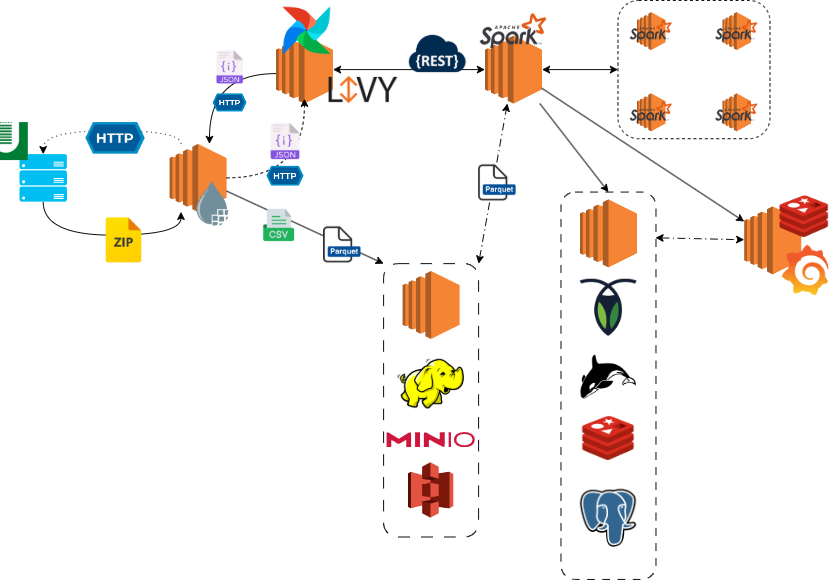
\includegraphics[width=0.67\textwidth]{../Report/graphs/InteractionDiagram}
    \caption{Il diagramma di interazione mostra le componenti chiave di SAE e le loro interazioni durante l'esecuzione di un job Spark, dall'ingestion dei dati alla persistenza dei risultati.}
    \label{fig:interaction_diagram}
\end{figure}

\begin{figure}[!htbp]
    \centering
    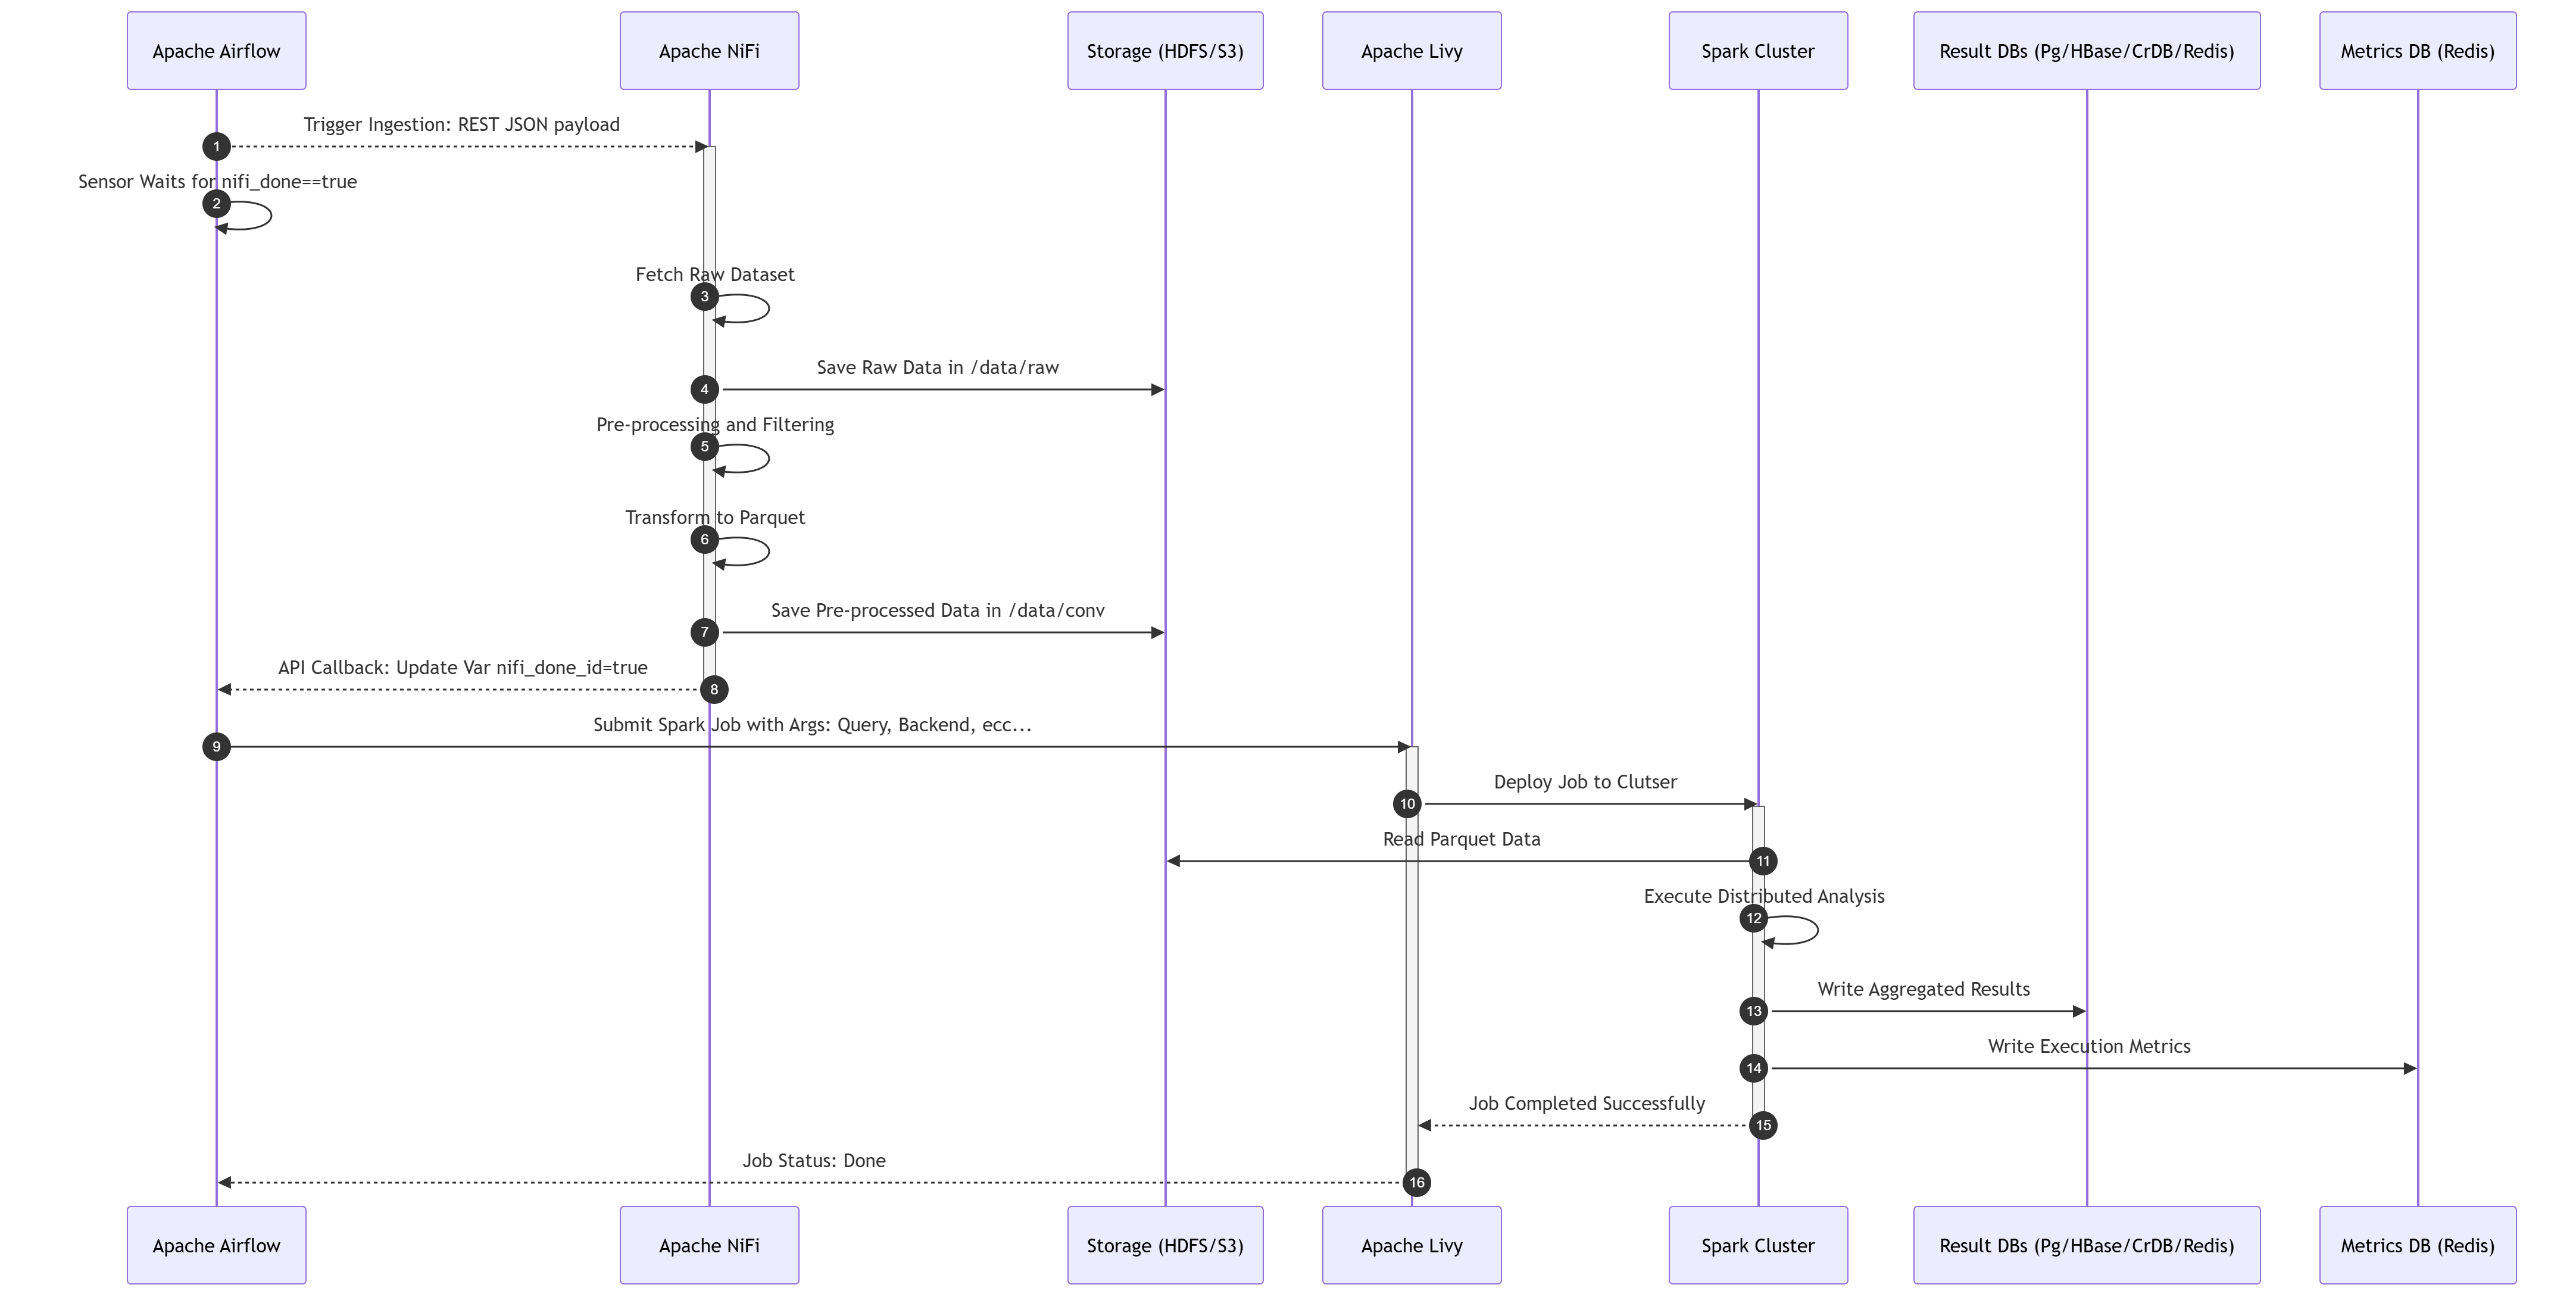
\includegraphics[width=0.9\textwidth]{../Report/graphs/sequence_diagram}
    \caption{Il diagramma di sequenza illustra la coreografia temporale delle chiamate API, l'ingestion asincrona e il ciclo di vita del job Spark all'interno della piattaforma.}
    \label{fig:sequence_diagram}
\end{figure}

\clearpage


\section{Rappresentazione grafica dei DAG di Spark}\label{sec:appendix_spark_dags}
In questa appendice vengono riportati i Directed Acyclic Graphs generati da Spark per le implementazioni RDD delle prime tre query.
Questi grafici illustrano le fasi di trasformazione, gli shuffle e la suddivisione in stage del piano di esecuzione distribuito.

\begin{figure}[!htbp]
    \centering
    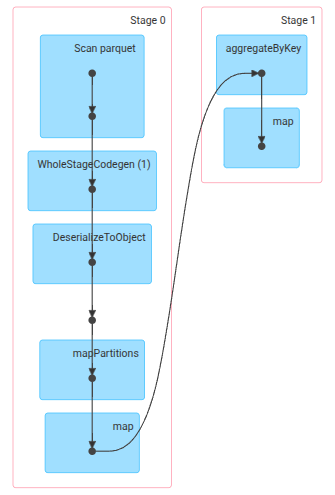
\includegraphics[width=0.6\textwidth]{../Results/charts/spark_dag/monthly_performance_rdd}
    \caption{DAG di Spark per la Query 1: evidenzia la fase di \textit{aggregateByKey} e la successiva trasformazione finale.}
    \label{fig:dag_q1}
\end{figure}

\begin{figure}[!htbp]
    \centering
    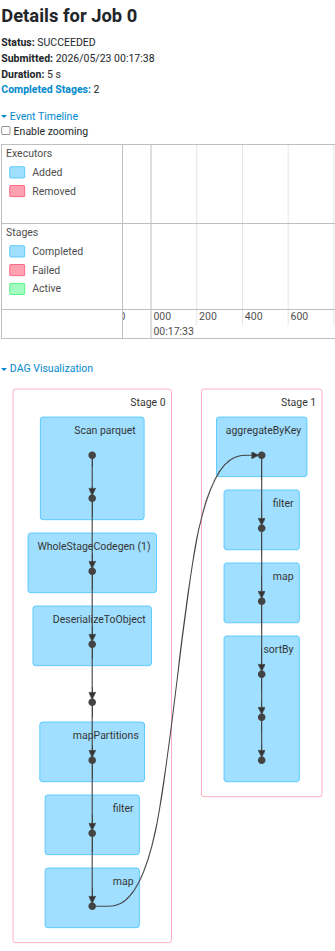
\includegraphics[width=0.255\textwidth]{../Results/charts/spark_dag/Query2_job0_rdd}
    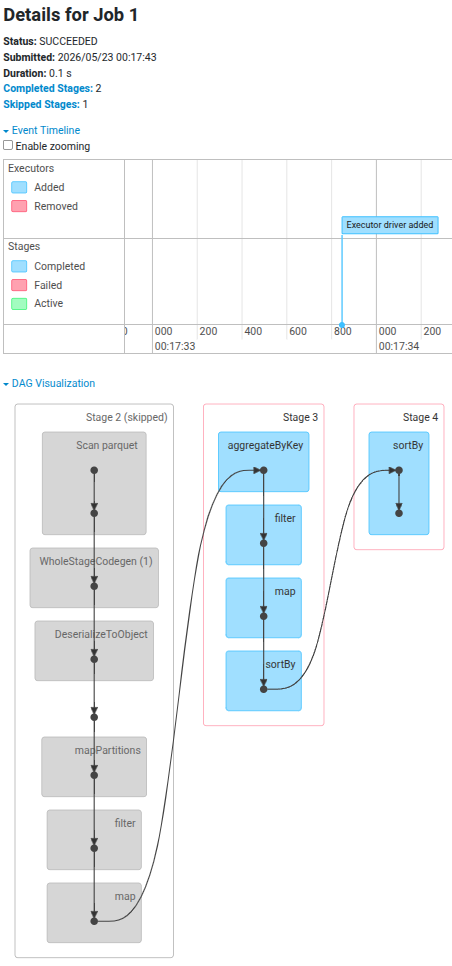
\includegraphics[width=0.34\textwidth]{../Results/charts/spark_dag/Query2_job1_rdd}
    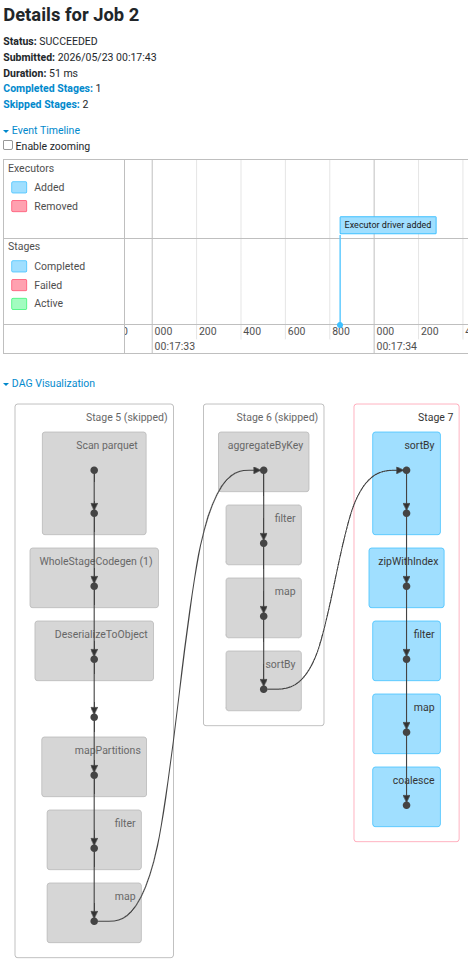
\includegraphics[width=0.35\textwidth]{../Results/charts/spark_dag/Query2_job2_rdd}
    \caption{DAG di Spark per la Query 2: i tre job mostrano rispettivamente il filtraggio/aggregazione, il calcolo delle medie e l'ordinamento per il ranking top-10.}
    \label{fig:dag_q2}
\end{figure}

\begin{figure*}[!htbp]
    \centering
    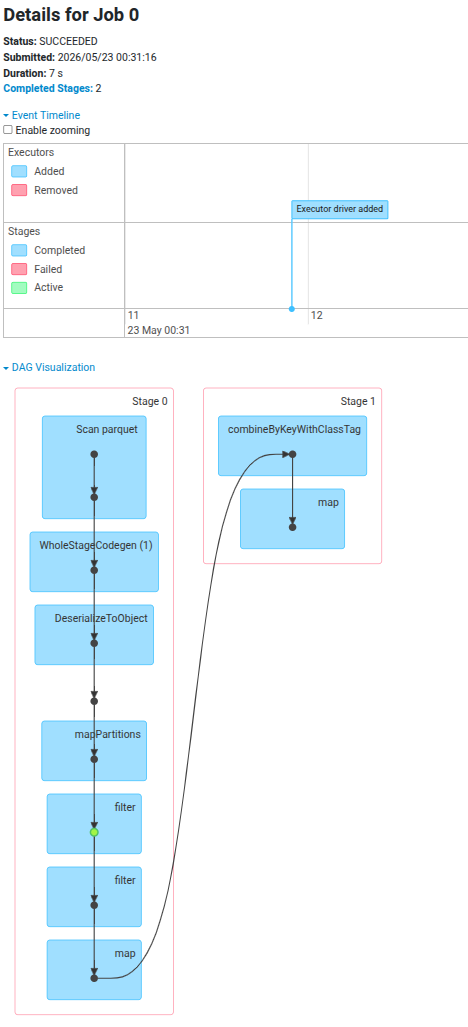
\includegraphics[width=0.41\textwidth]{../Results/charts/spark_dag/Query3_job0_rdd}
    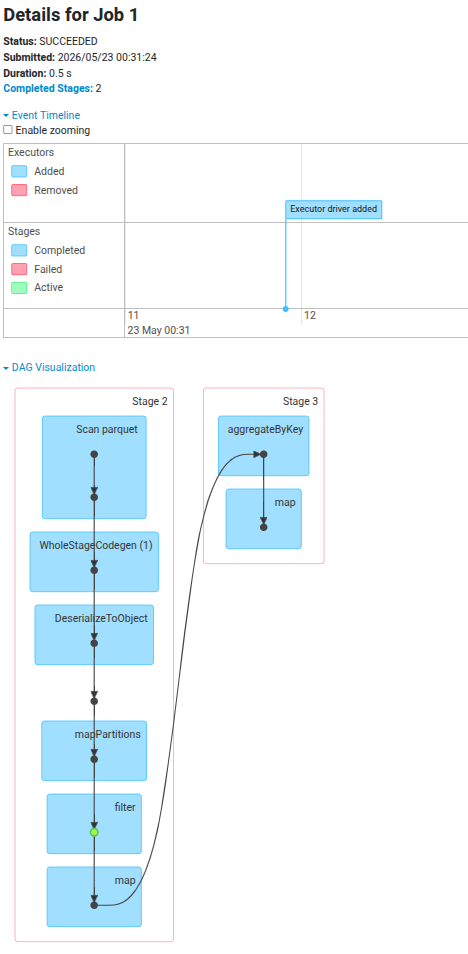
\includegraphics[width=0.44\textwidth]{../Results/charts/spark_dag/Query3_job1_rdd}
    \caption{DAG di Spark per la Query 3: i due job paralleli gestiscono rispettivamente la pipeline degli sketch per i percentili e la pipeline per il calcolo dei minimi e massimi globali.}
    \label{fig:dag_q3}
\end{figure*}

\clearpage

\section{Dettaglio dei Tempi di Esecuzione}\label{sec:appendix_telemetry}
In questa appendice vengono riportati in dettaglio i pannelli di telemetria estratti dalle dashboard di Grafana, relativi ai tempi di esecuzione delle quattro query di processamento Spark. 

Ogni pannello all'interno della plancia di monitoraggio è posizionato in modo da fornire una visione granulare delle performance del sistema, organizzato su tre livelli logici:
\begin{itemize}
    \item \textbf{Spark vs Wall Clock Execution Time (In alto a sinistra):} Un grafico che confronta l'overhead misurato tramite \texttt{System.currentTimeMillis()} sul driver Java con il tempo di esecuzione effettivo dei job intercettato dai listener di Spark.
    Il divario evidenzia il tempo speso per lo scheduling e la negoziazione delle risorse.
    \item \textbf{Distribuzione Statistica dello Spark Time (In alto al centro):} Mostra la dispersione statistica dei tempi di calcolo di Spark attraverso le diverse run, permettendo di identificare la stabilità delle performance per il backend selezionato.
    \item \textbf{Active Executors (In alto a di destra):} Indica il numero medio di nodi executor che hanno partecipato attivamente alla computazione durante le varie esecuzioni del benchmark.
    \item \textbf{Stage Breakdown (Al centro a sinistra):} Uno spaccato temporale dettagliato che scompone l'esecuzione nei singoli stage di computazione di Spark, utile per isolare la fase logica della query che presenta la latenza maggiore.
    \item \textbf{Execution Stages (Al centro a destra):} Rappresenta il numero medio di stage generati dall'ottimizzatore di Spark durante le esecuzioni, fornendo un'indicazione della complessità del piano fisico.
    \item \textbf{I/O Throughput (In basso a sinistra):} Monitoraggio del volume di dati letti e scritti su disco/HDFS/S3, che permette di valutare l'impatto delle operazioni di input/output persistente.
    \item \textbf{Shuffle I/O (In basso al centro):} Analisi del traffico dati generato esclusivamente durante le fasi di shuffle per la redistribuzione dei record tra i nodi del cluster.
    \item \textbf{Executor Workload Skew (In basso a destra):} Valuta il bilanciamento del carico tra i nodi.
    Il grafico confronta il valore medio dei byte letti (caso ideale di distribuzione uniforme, in verde) con il valore massimo letto da un singolo nodo (in rosso), evidenziando lo sbilanciamento del carico di lavoro rispetto alla configurazione ideale.
\end{itemize}

\clearpage

\subsection{Query 1: Statistiche Mensili}

\begin{figure}[!htbp]
    \centering
    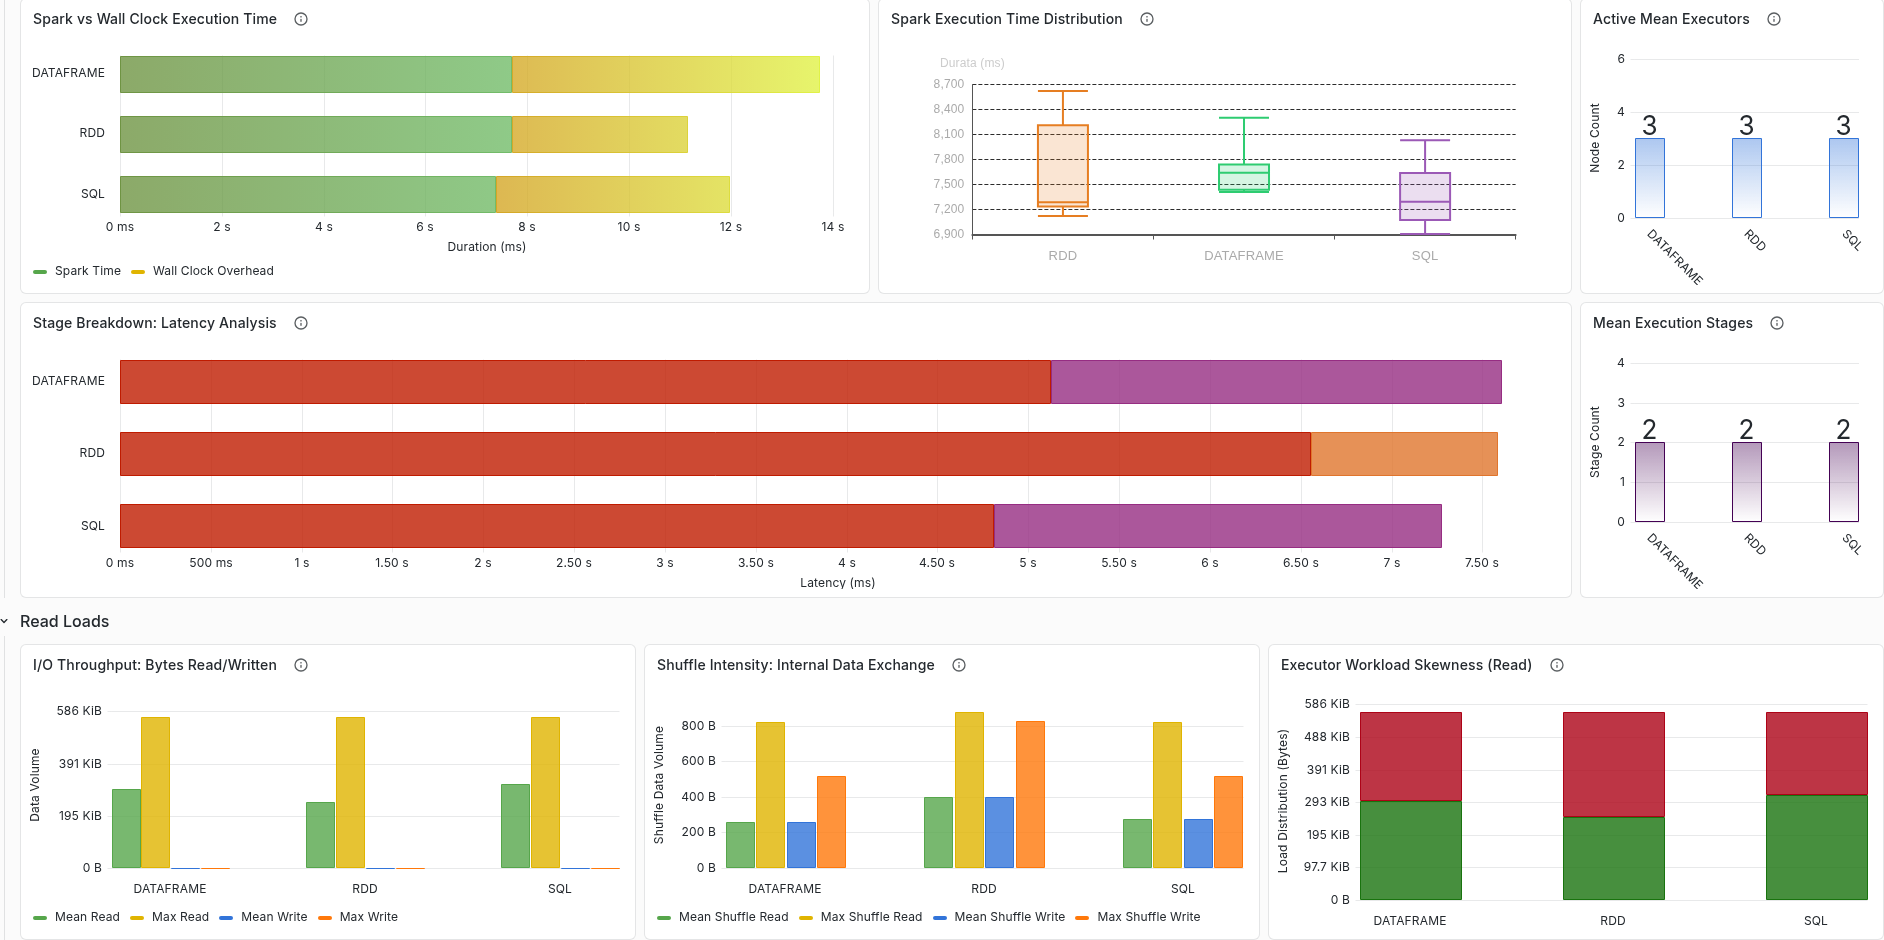
\includegraphics[width=1\textwidth]{../Results/charts/telemetry/ec2/part_prun/metrics_ec2_monthly_performance_part_prun_cropped}

    \vspace{1cm}

    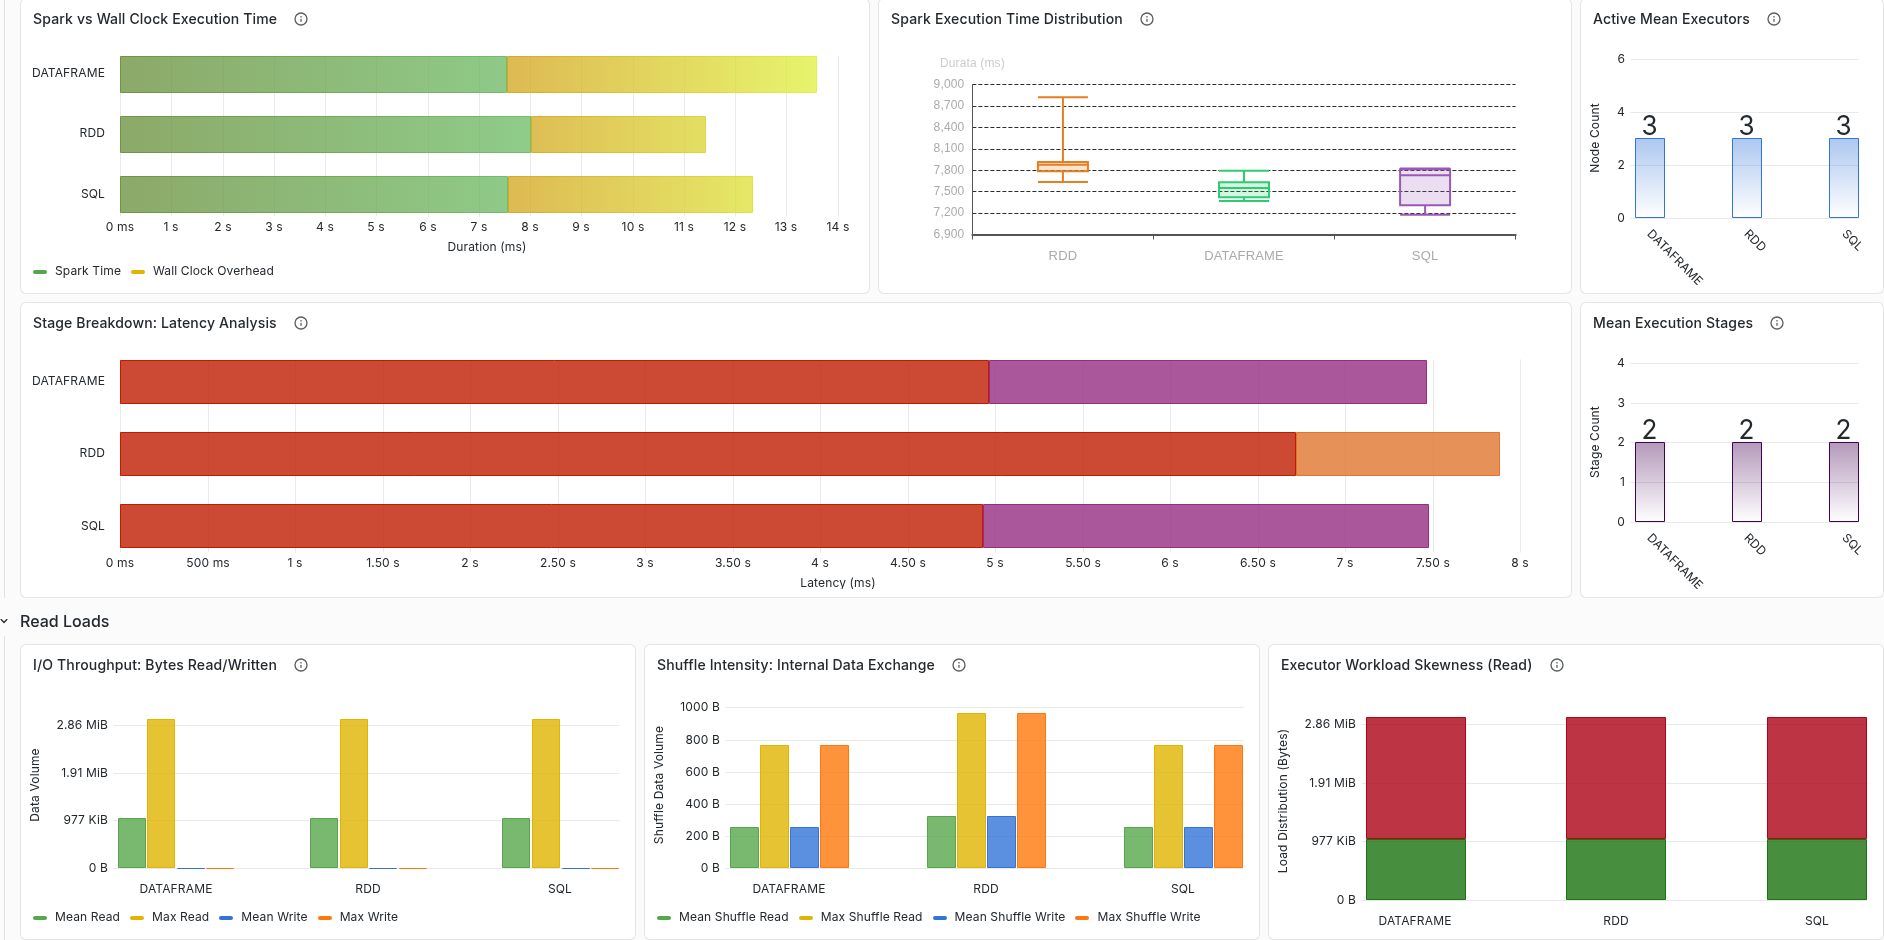
\includegraphics[width=1\textwidth]{../Results/charts/telemetry/ec2/pred_push/metrics_ec2_monthly_performance_pred_push_cropped}
    \caption{Telemetria Query 1 su AWS EC2: Partition Pruning (sopra) vs Predicate Pushdown (sotto).}
    \label{fig:telemetry_q1_ec2}
\end{figure}

\clearpage

\begin{figure}[!htbp]
    \centering
    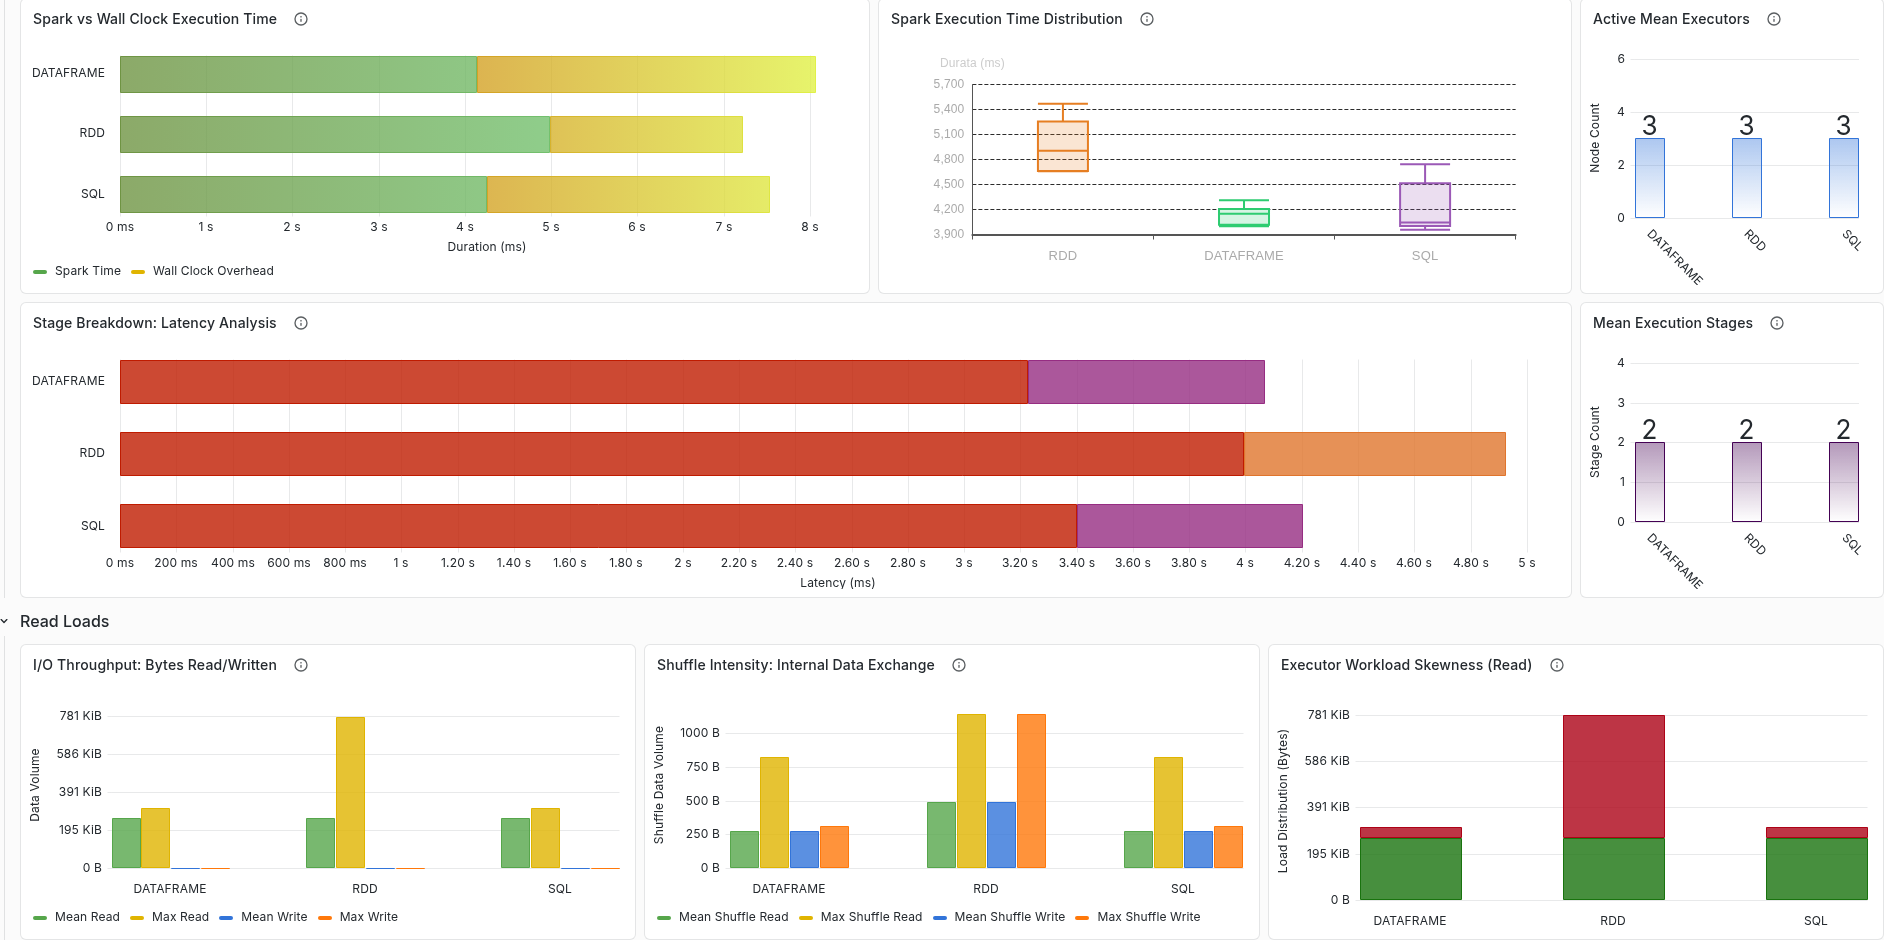
\includegraphics[width=1\textwidth]{../Results/charts/telemetry/emr/part_prun/metrics_emr_monthly_performance_part_prun_cropped}

    \vspace{1cm}

    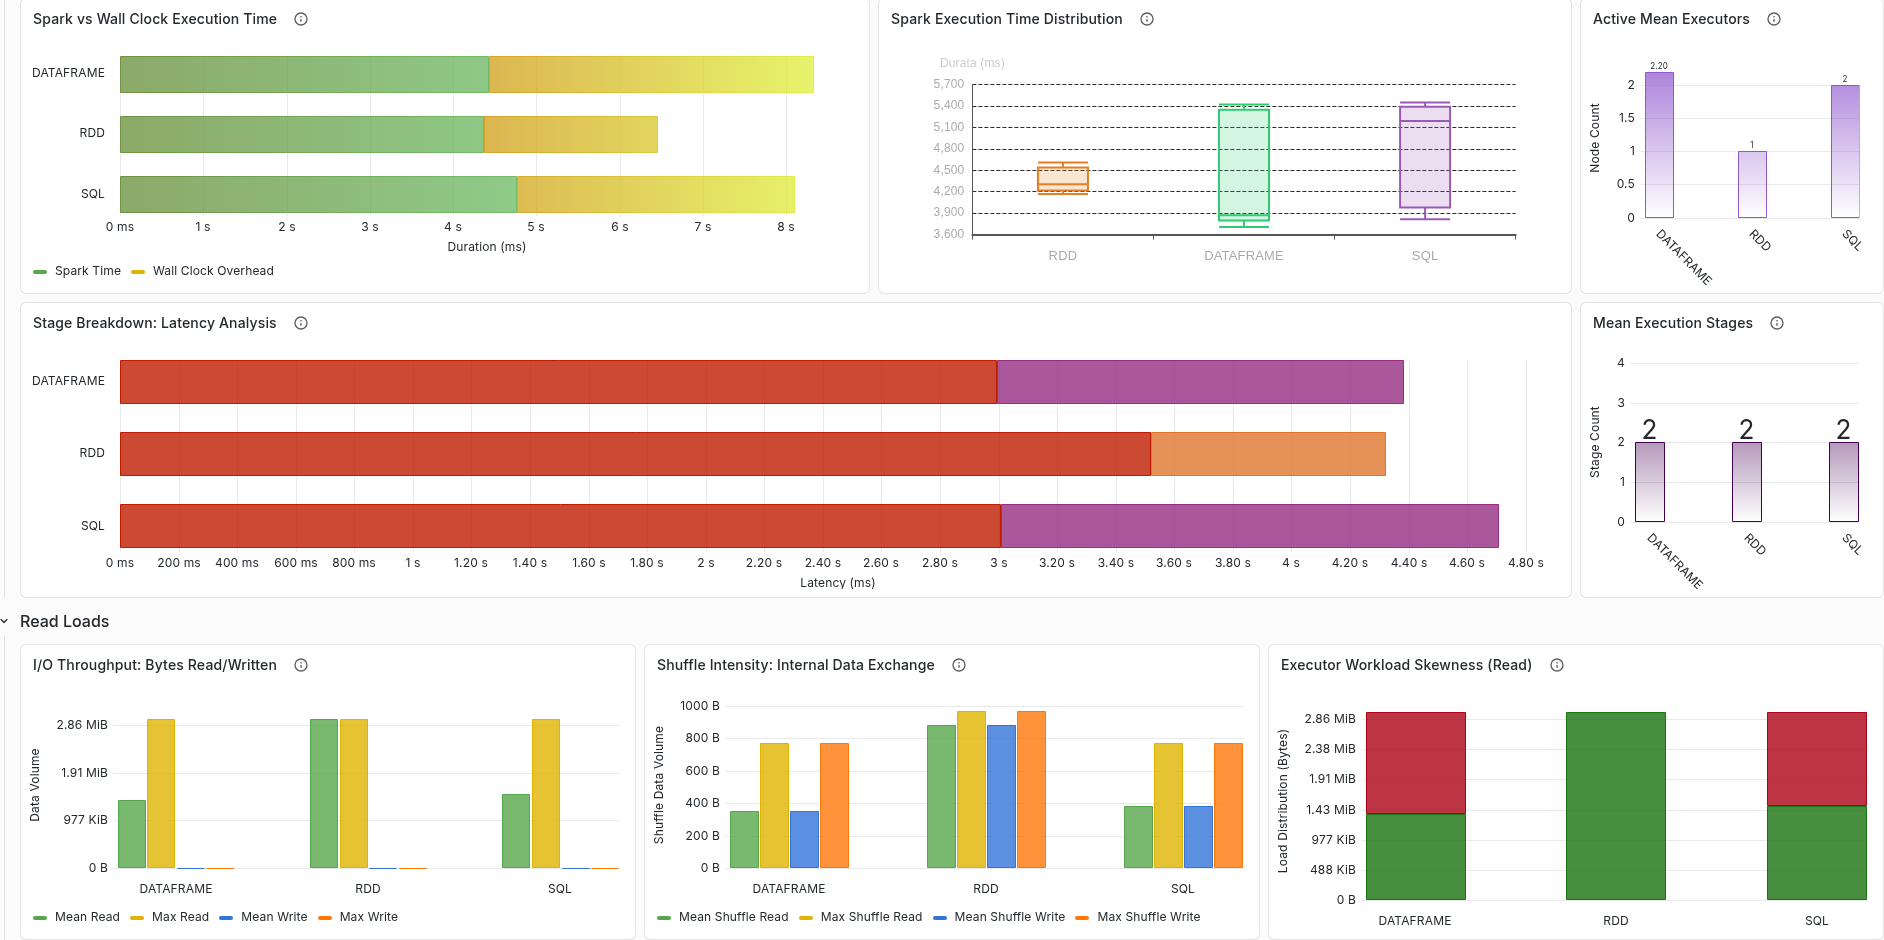
\includegraphics[width=1\textwidth]{../Results/charts/telemetry/emr/pred_push/metrics_emr_monthly_performance_pred_push_cropped}
    \caption{Telemetria Query 1 su AWS EMR: Partition Pruning (sopra) vs Predicate Pushdown (sotto).}
    \label{fig:telemetry_q1_emr}
\end{figure}

\clearpage

\subsection{Query 2: Decomposizione dei Ritardi}

\begin{figure}[!htbp]
    \centering
    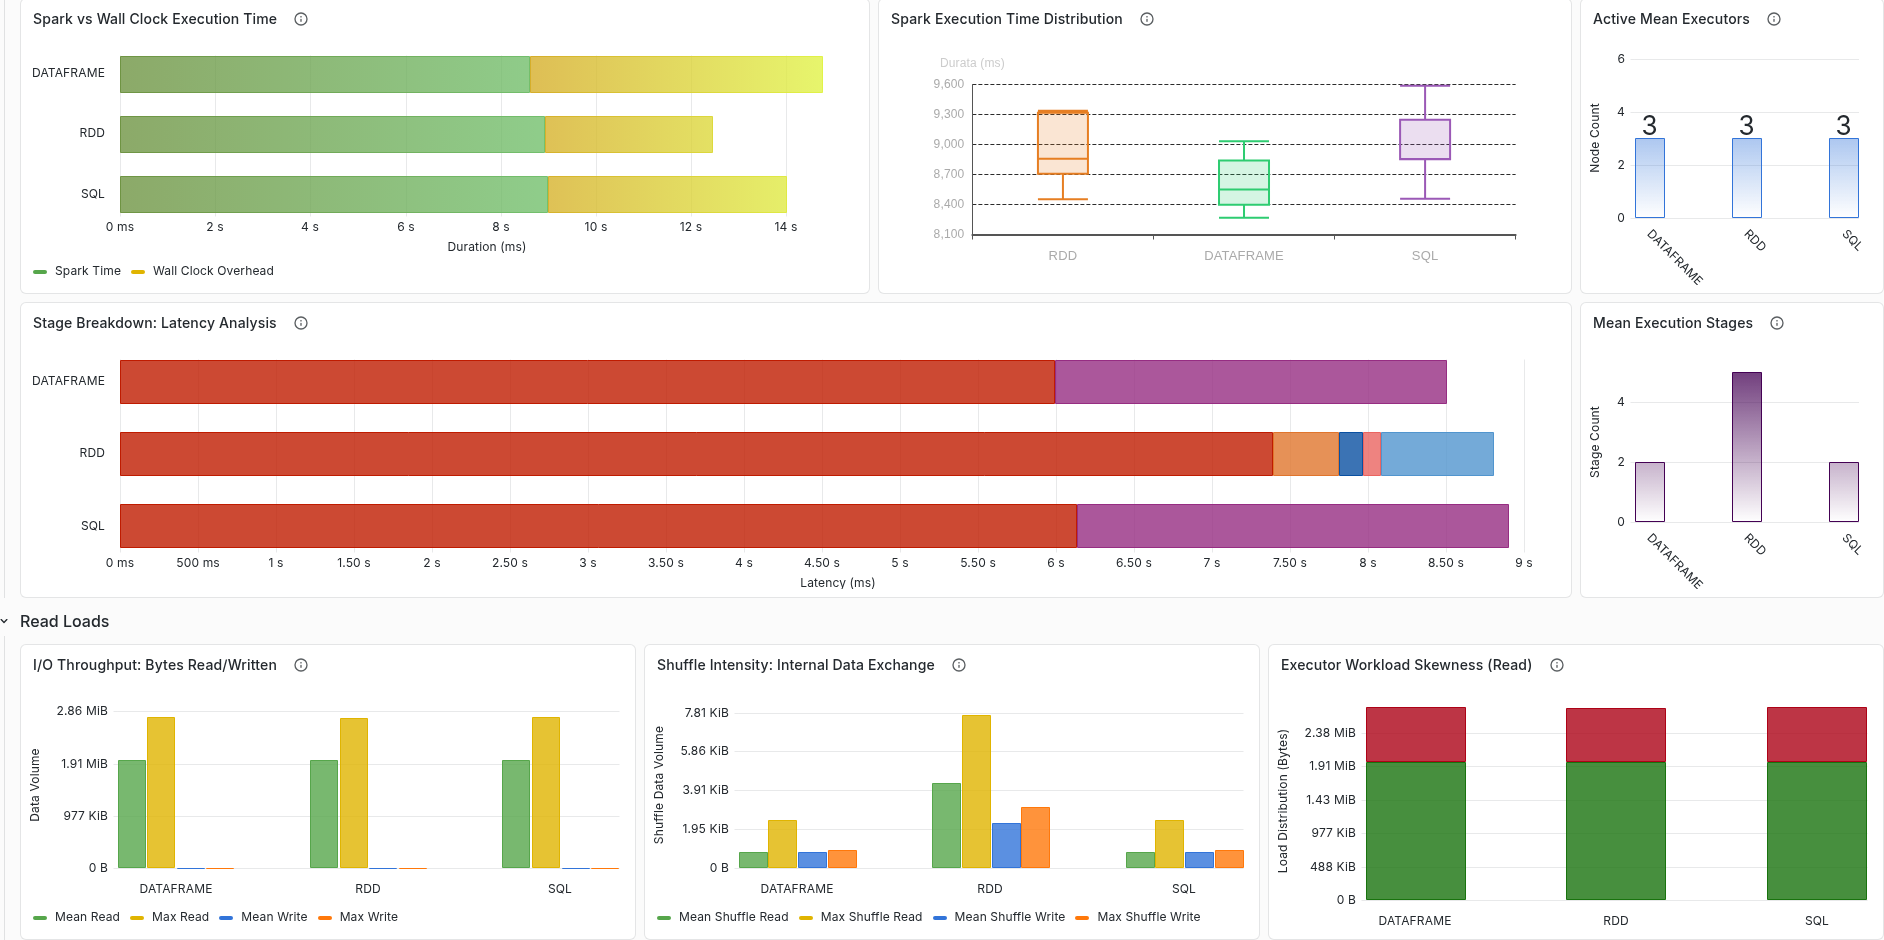
\includegraphics[width=1\textwidth]{../Results/charts/telemetry/ec2/part_prun/metrics_ec2_arrival_delay_ranking_part_prun_cropped}

    \vspace{1cm}

    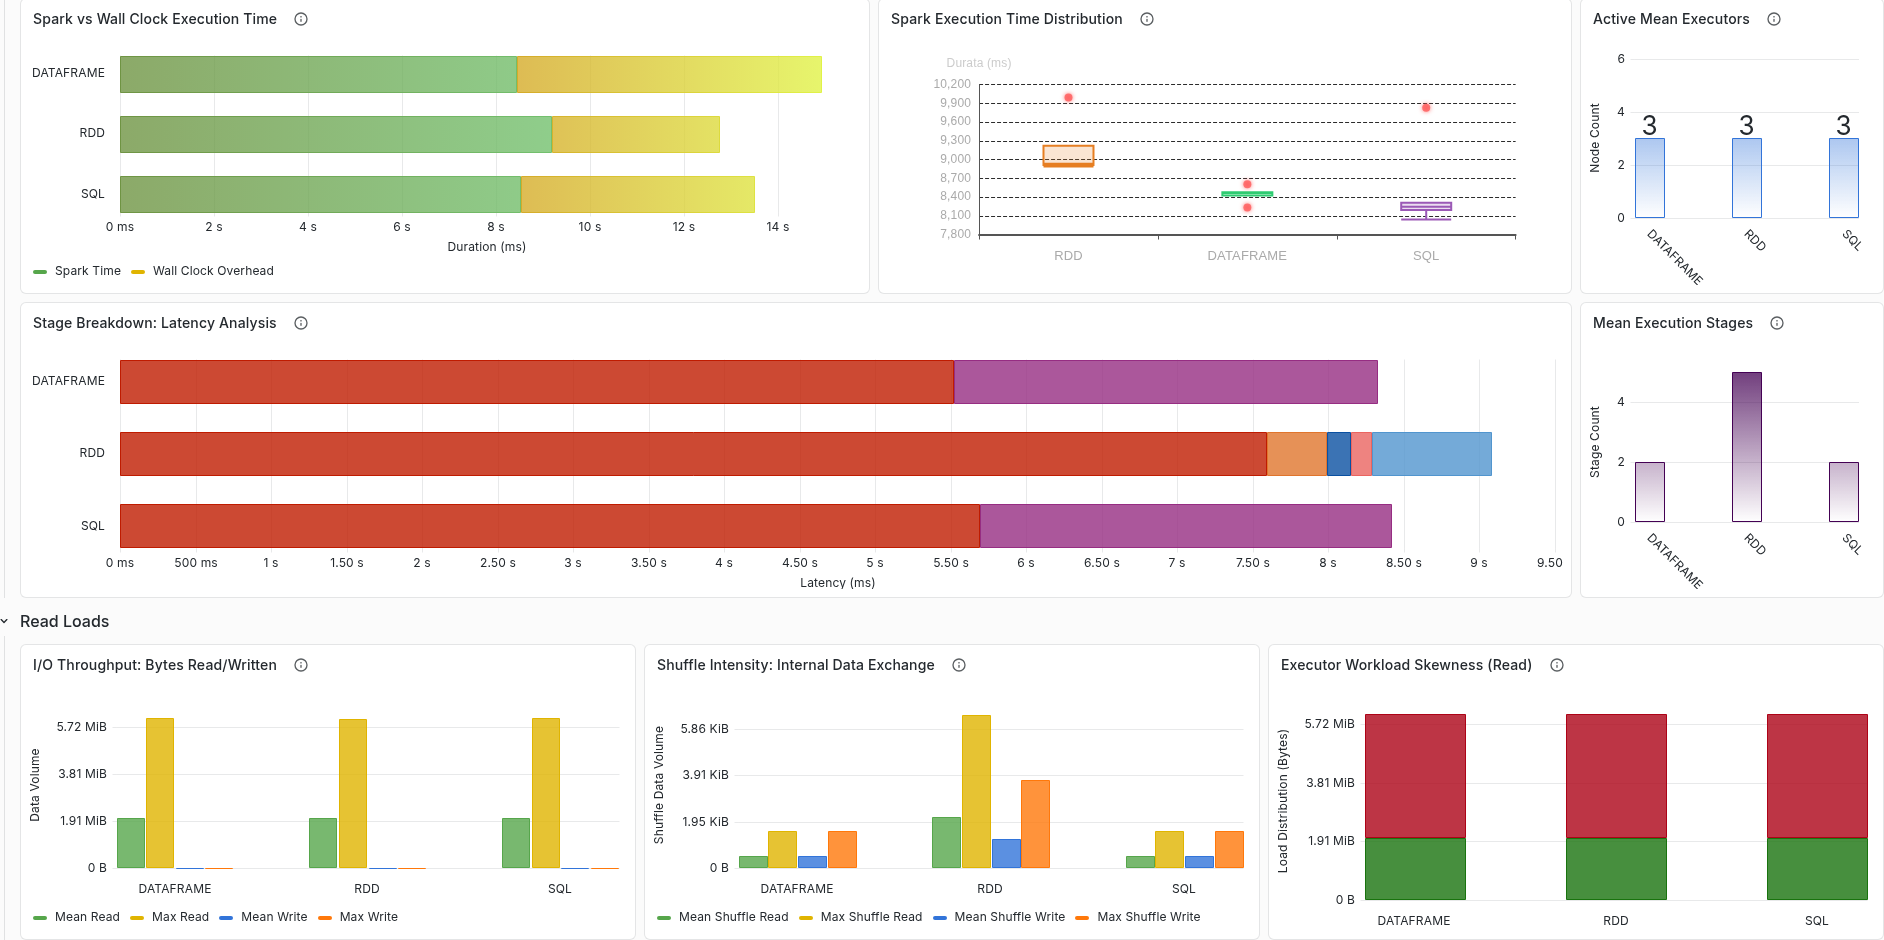
\includegraphics[width=1\textwidth]{../Results/charts/telemetry/ec2/pred_push/metrics_ec2_arrival_delay_ranking_pred_push_cropped}
    \caption{Telemetria Query 2 su AWS EC2: Partition Pruning (sopra) vs Predicate Pushdown (sotto).}
    \label{fig:telemetry_q2_ec2}
\end{figure}

\clearpage

\begin{figure}[!htbp]
    \centering
    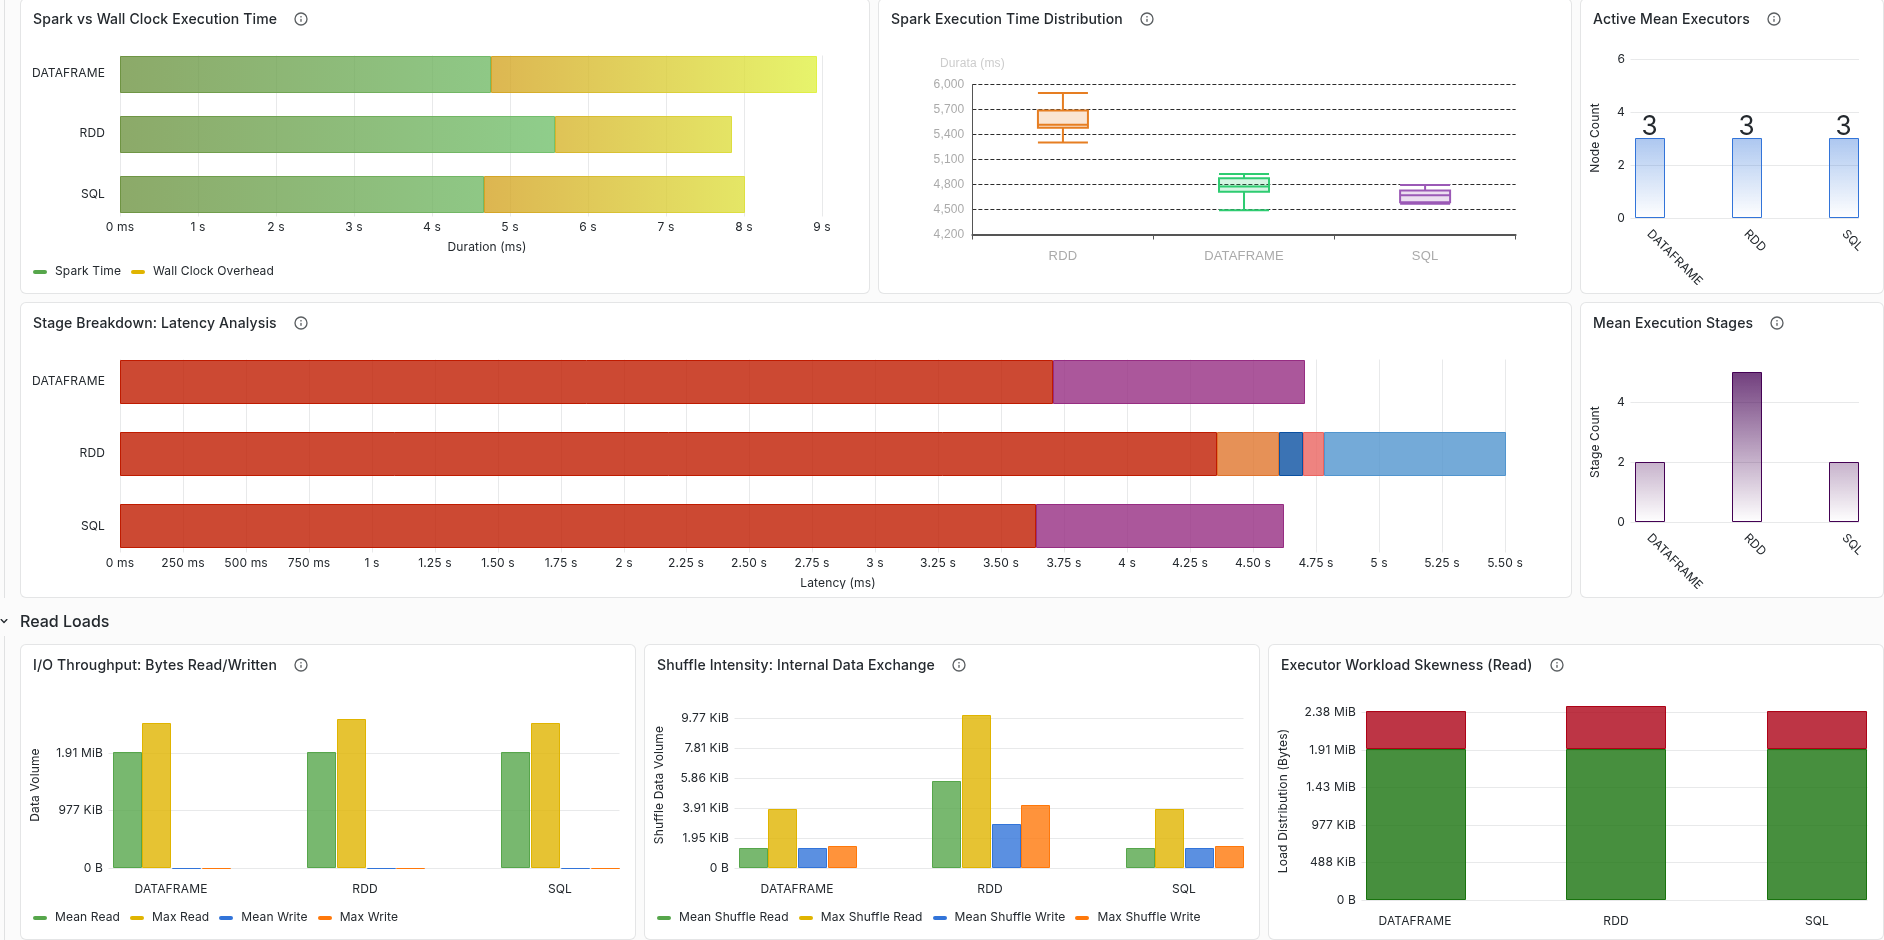
\includegraphics[width=1\textwidth]{../Results/charts/telemetry/emr/part_prun/metrics_emr_arrival_delay_ranking_part_prun_cropped}

    \vspace{1cm}

    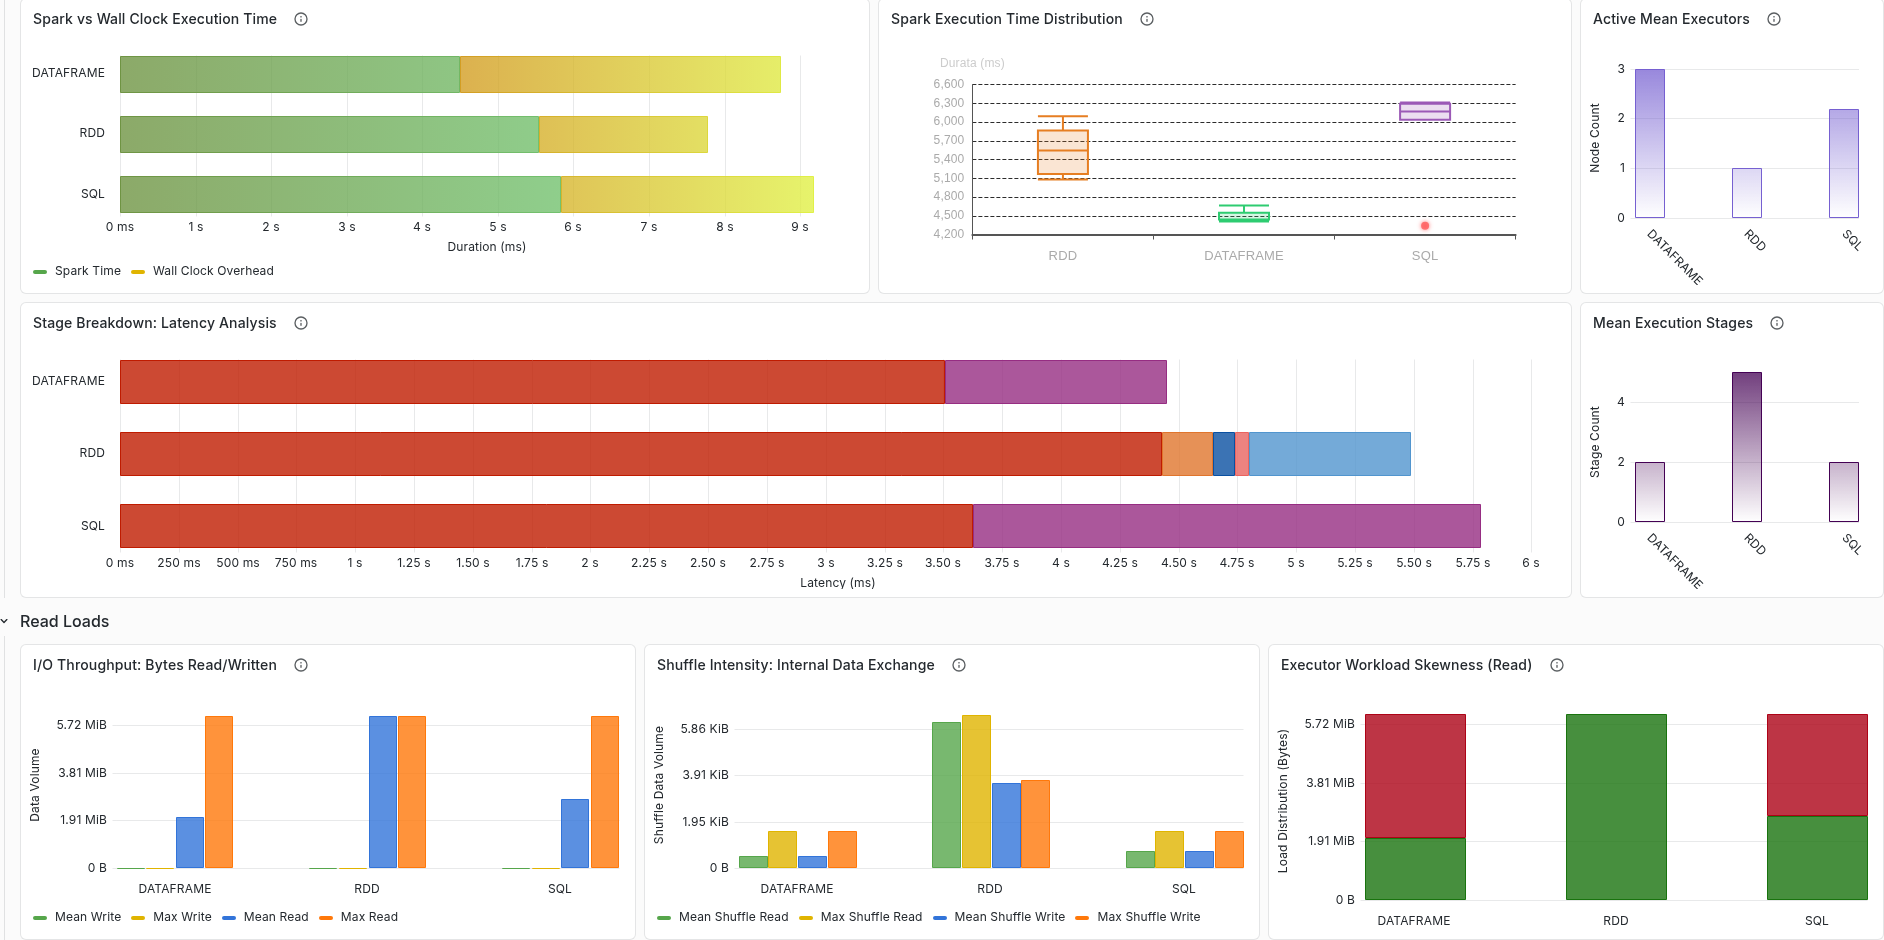
\includegraphics[width=1\textwidth]{../Results/charts/telemetry/emr/pred_push/metrics_emr_arrival_delay_ranking_pred_push_cropped}
    \caption{Telemetria Query 2 su AWS EMR: Partition Pruning (sopra) vs Predicate Pushdown (sotto).}
    \label{fig:telemetry_q2_emr}
\end{figure}

\clearpage

\subsection{Query 3: Percentili per Fasce Orarie}

\begin{figure}[!htbp]
    \centering
    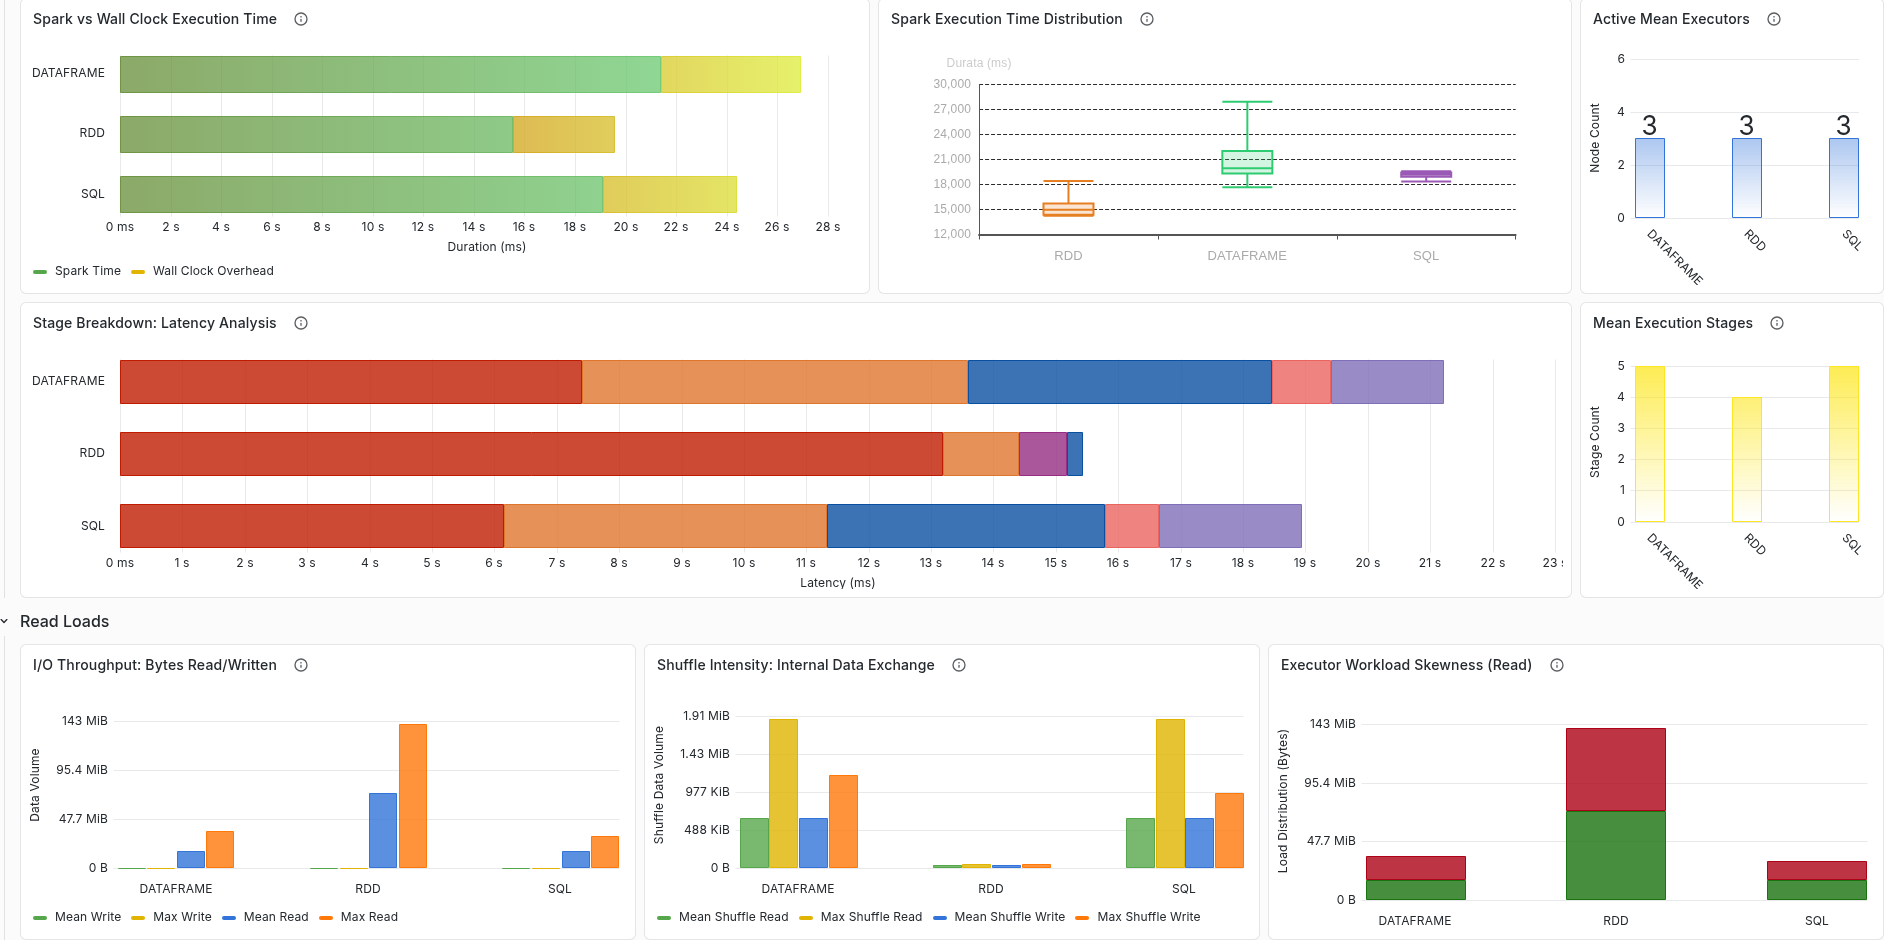
\includegraphics[width=1\textwidth]{../Results/charts/telemetry/ec2/part_prun/metrics_ec2_hourly_delay_percentiles_kll_part_prun_cropped}

    \vspace{1cm}

    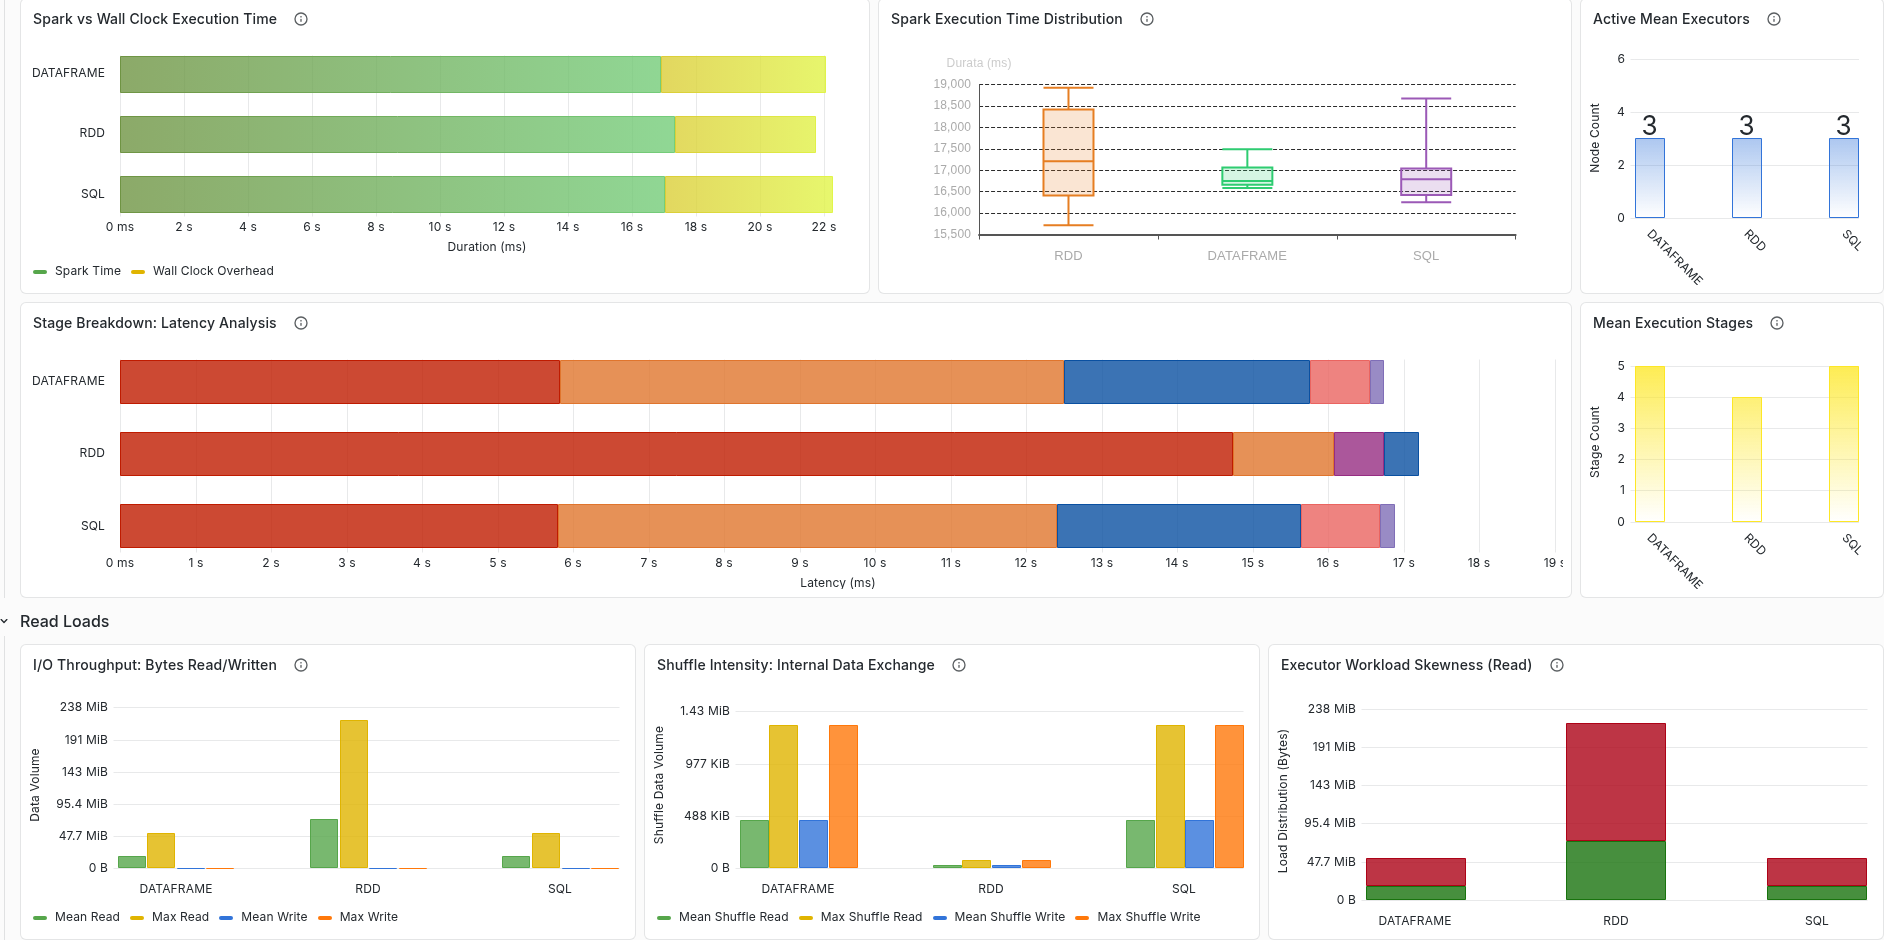
\includegraphics[width=1\textwidth]{../Results/charts/telemetry/ec2/pred_push/metrics_ec2_hourly_delay_percentiles_kll_pred_push_cropped}
    \caption{Telemetria Query 3 su AWS EC2 con algoritmo KLL: Partition Pruning (sopra) vs Predicate Pushdown (sotto).}
    \label{fig:telemetry_q3_kll_ec2}
\end{figure}

\clearpage

\begin{figure}[!htbp]
    \centering
    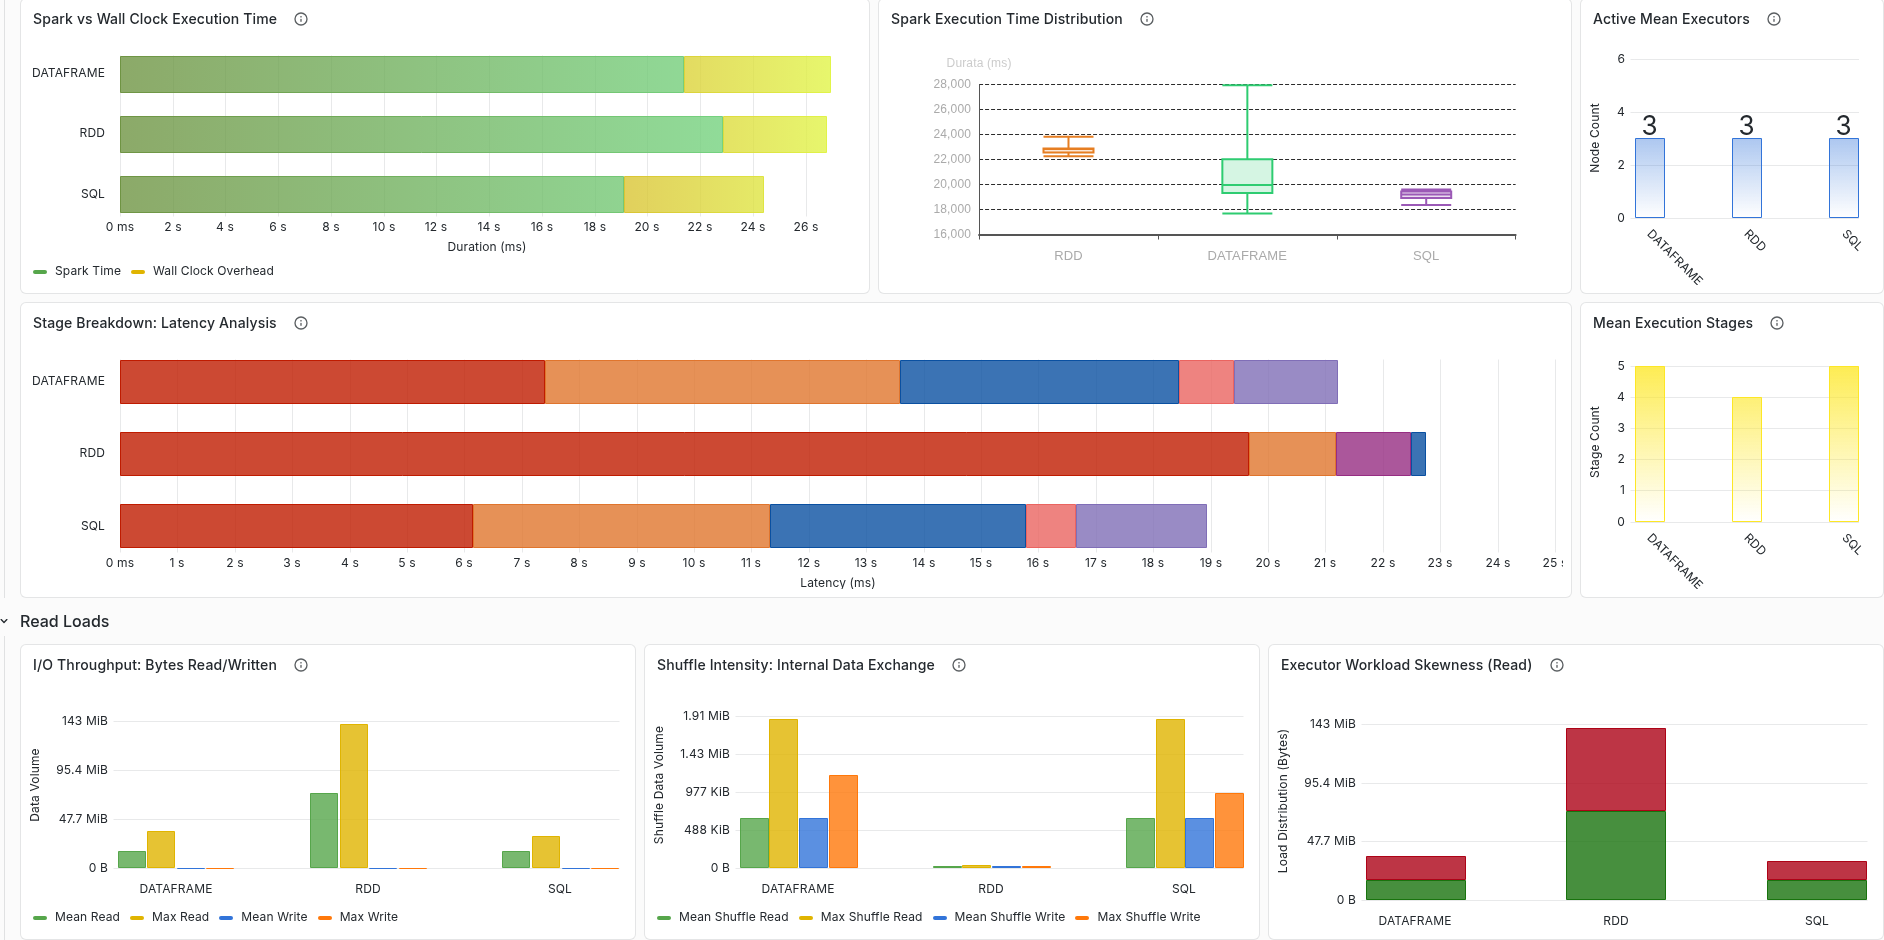
\includegraphics[width=1\textwidth]{../Results/charts/telemetry/ec2/part_prun/metrics_ec2_hourly_delay_percentiles_tdigest_part_prun_cropped}

    \vspace{1cm}

    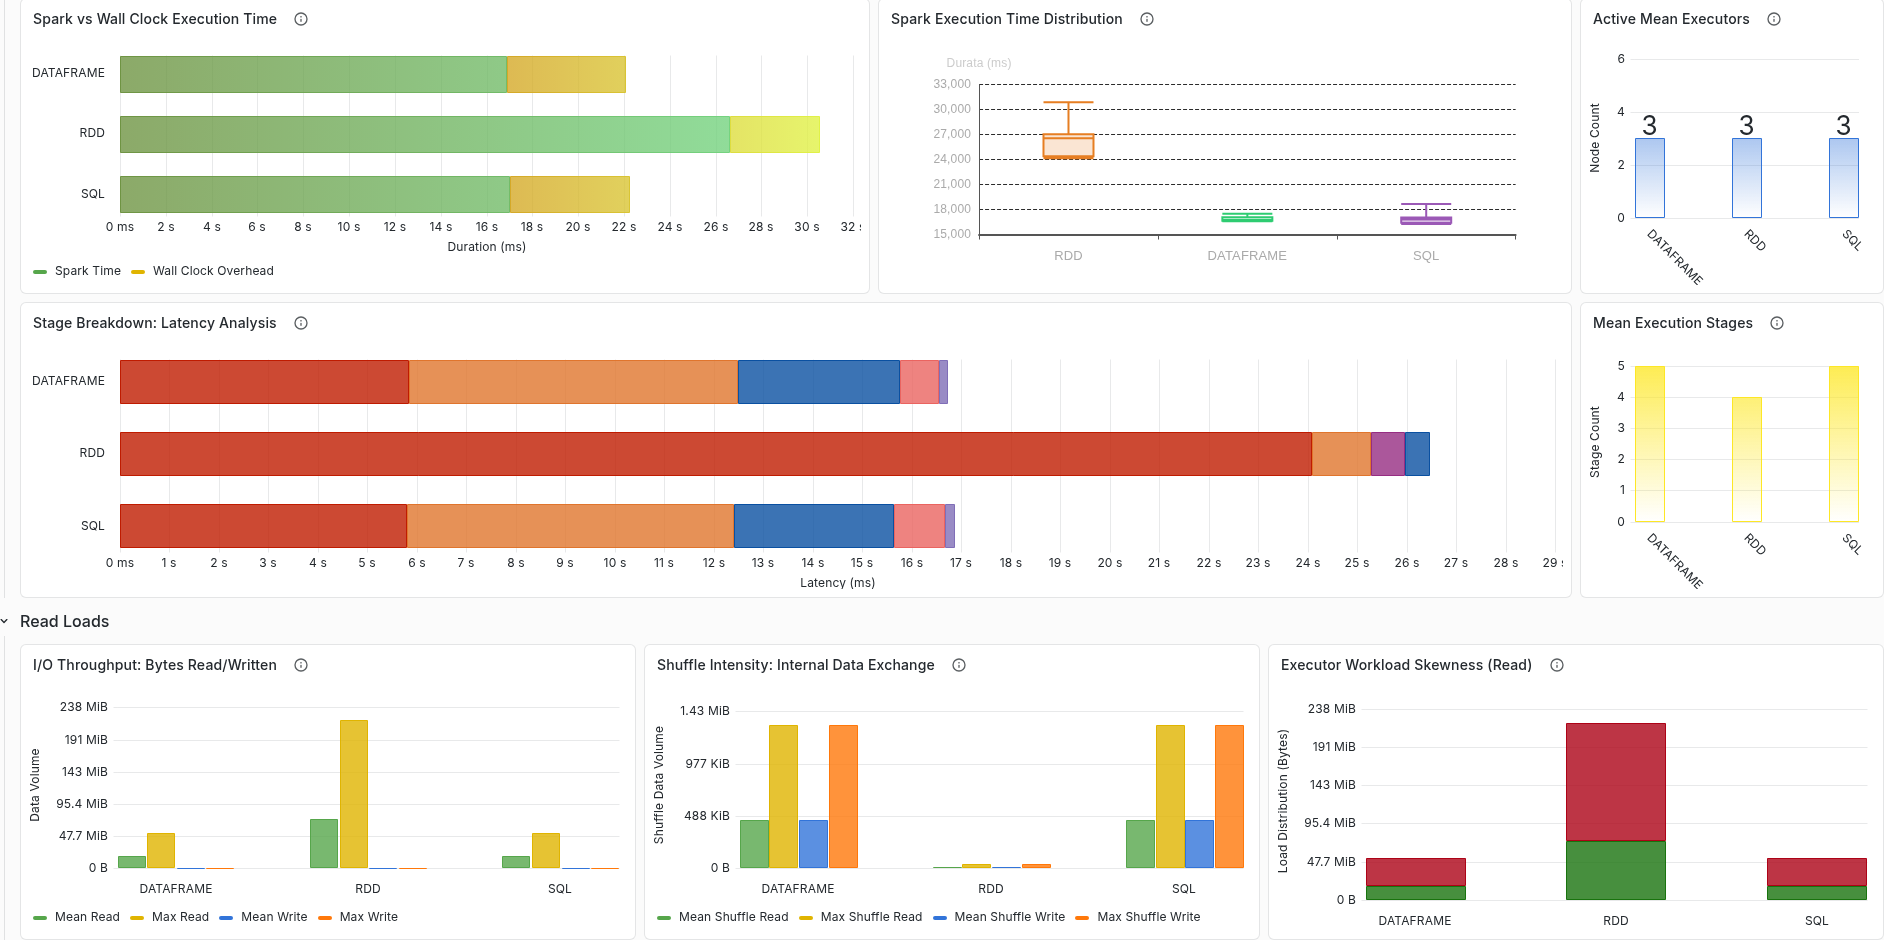
\includegraphics[width=1\textwidth]{../Results/charts/telemetry/ec2/pred_push/metrics_ec2_hourly_delay_percentiles_tdigest_pred_push_cropped}
    \caption{Telemetria Query 3 su AWS EC2 con algoritmo T-Digest: Partition Pruning (sopra) vs Predicate Pushdown (sotto).}
    \label{fig:telemetry_q3_tdigest_ec2}
\end{figure}

\clearpage

\begin{figure}[!htbp]
    \centering
    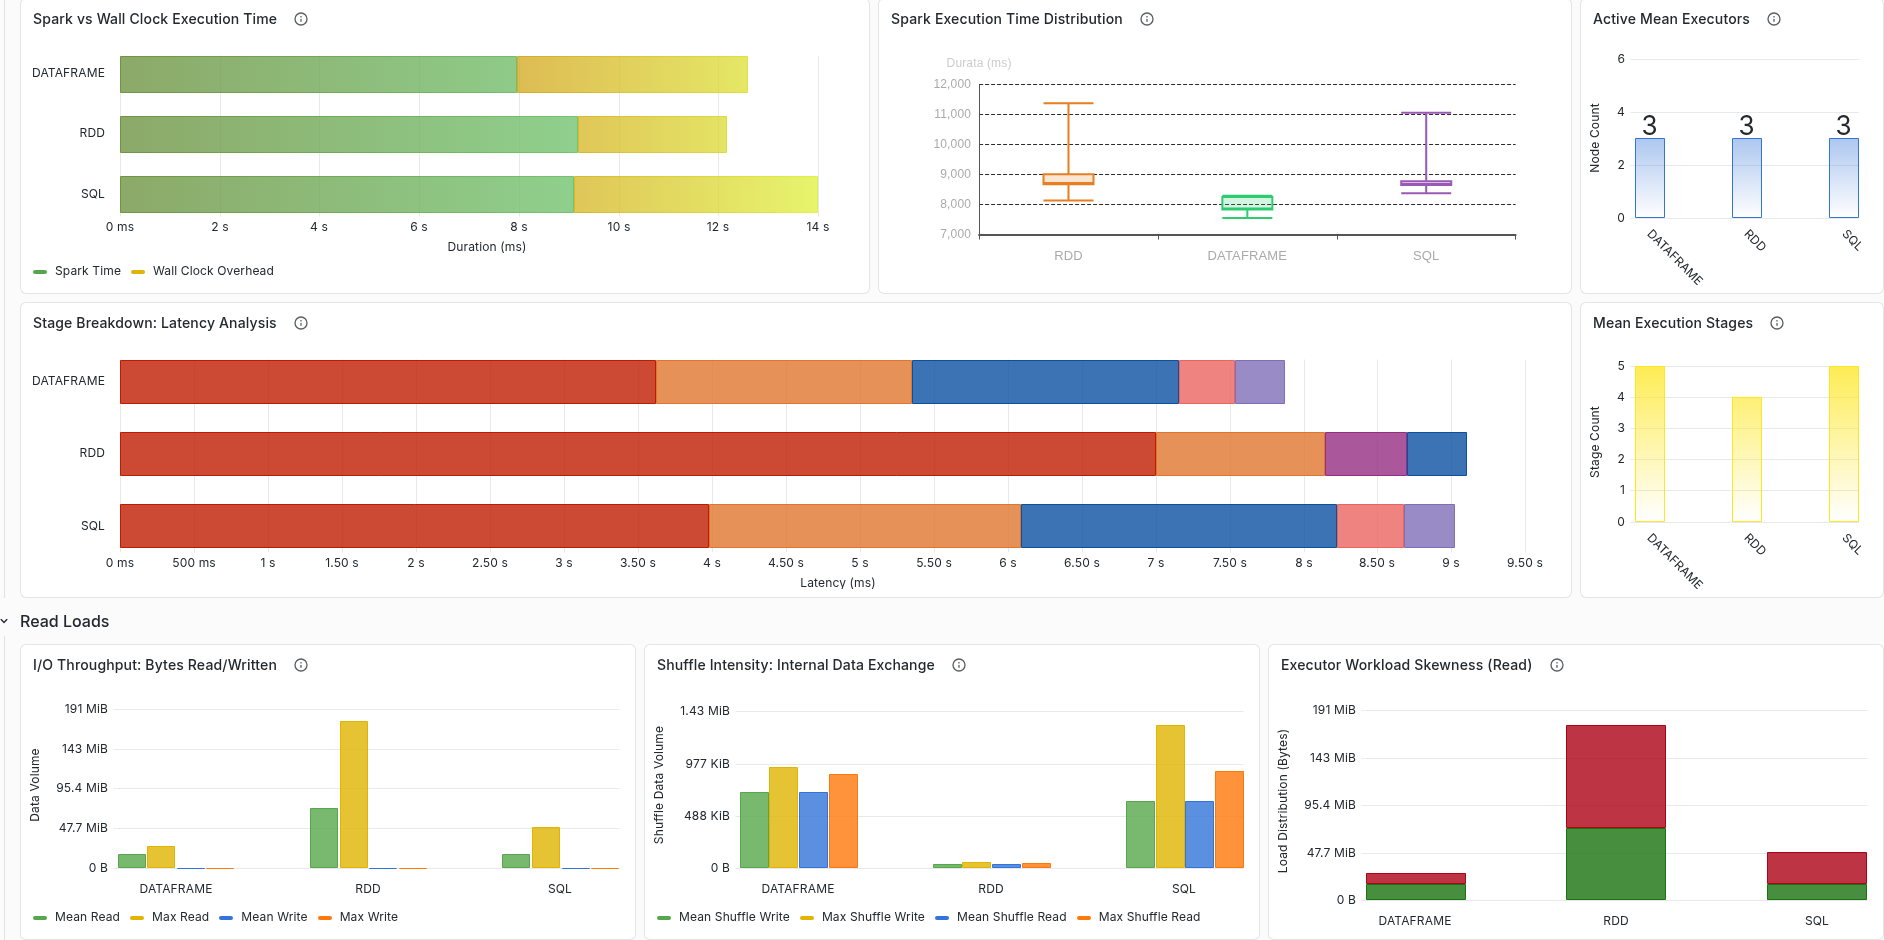
\includegraphics[width=1\textwidth]{../Results/charts/telemetry/emr/part_prun/metrics_emr_hourly_delay_percentiles_kll_part_prun_cropped}

    \vspace{1cm}

    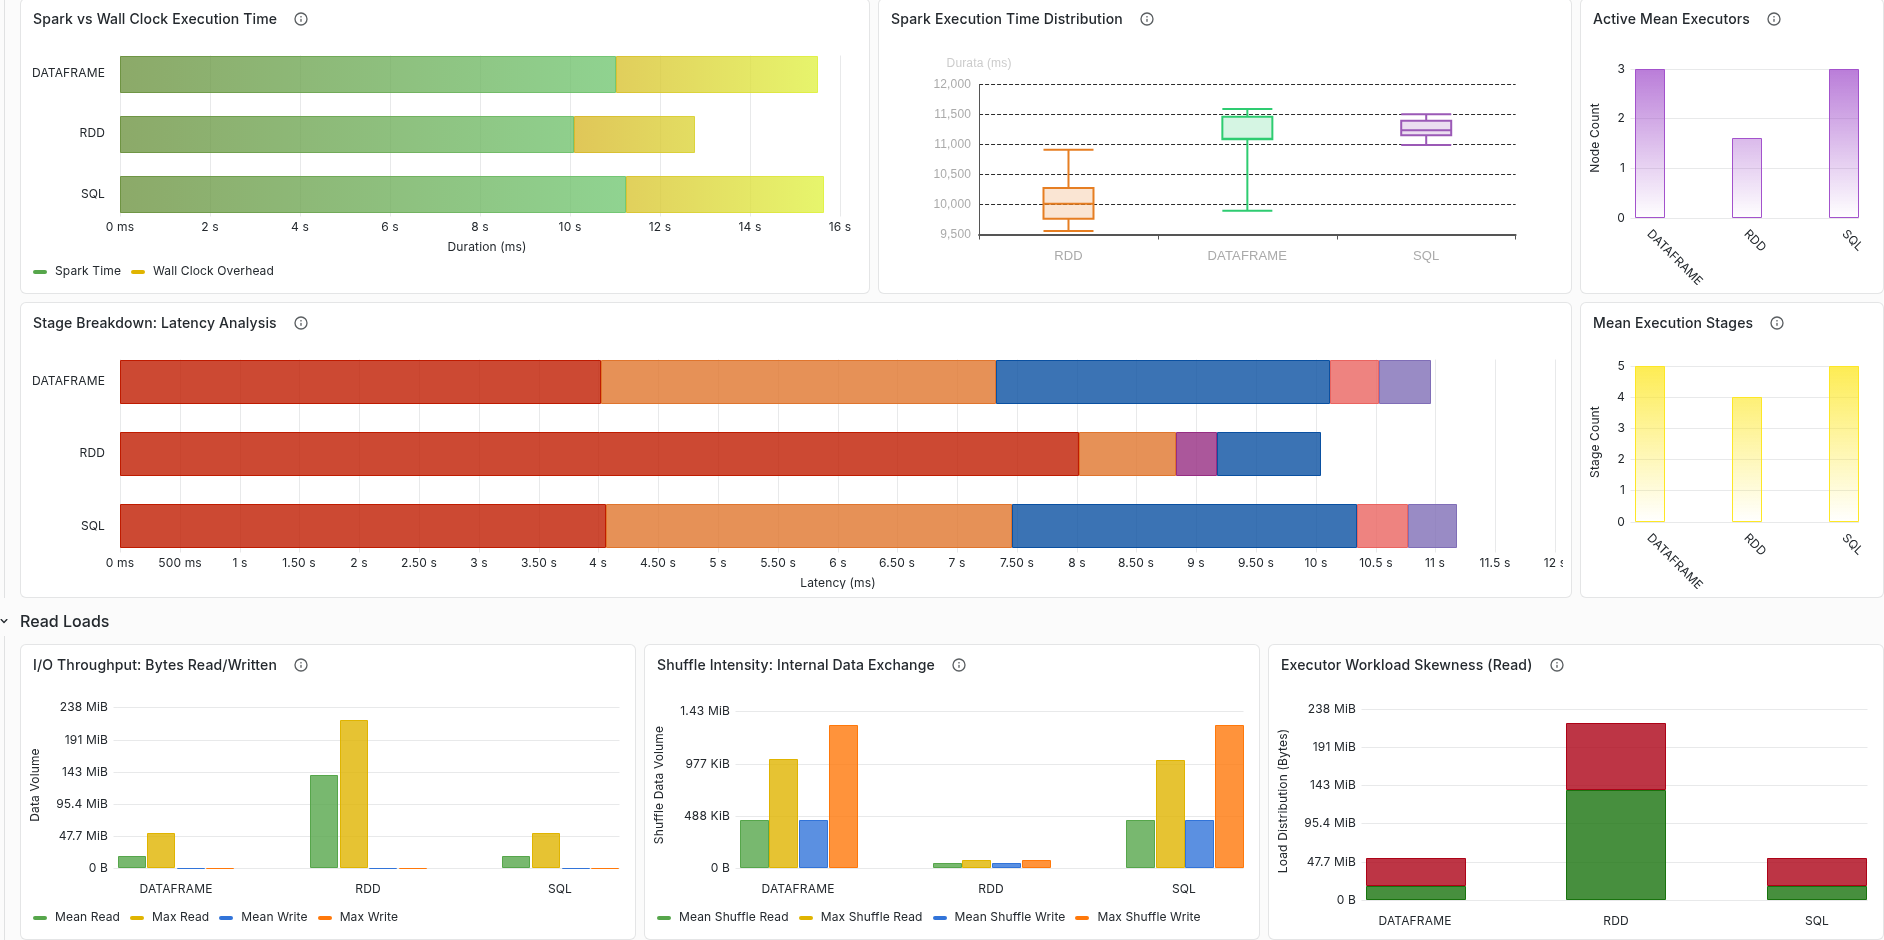
\includegraphics[width=1\textwidth]{../Results/charts/telemetry/emr/pred_push/metrics_emr_hourly_delay_percentiles_kll_pred_push_cropped}
    \caption{Telemetria Query 3 su AWS EMR con algoritmo KLL: Partition Pruning (sopra) vs Predicate Pushdown (sotto).}
    \label{fig:telemetry_q3_kll_emr}
\end{figure}

\clearpage

\begin{figure}[!htbp]
    \centering
    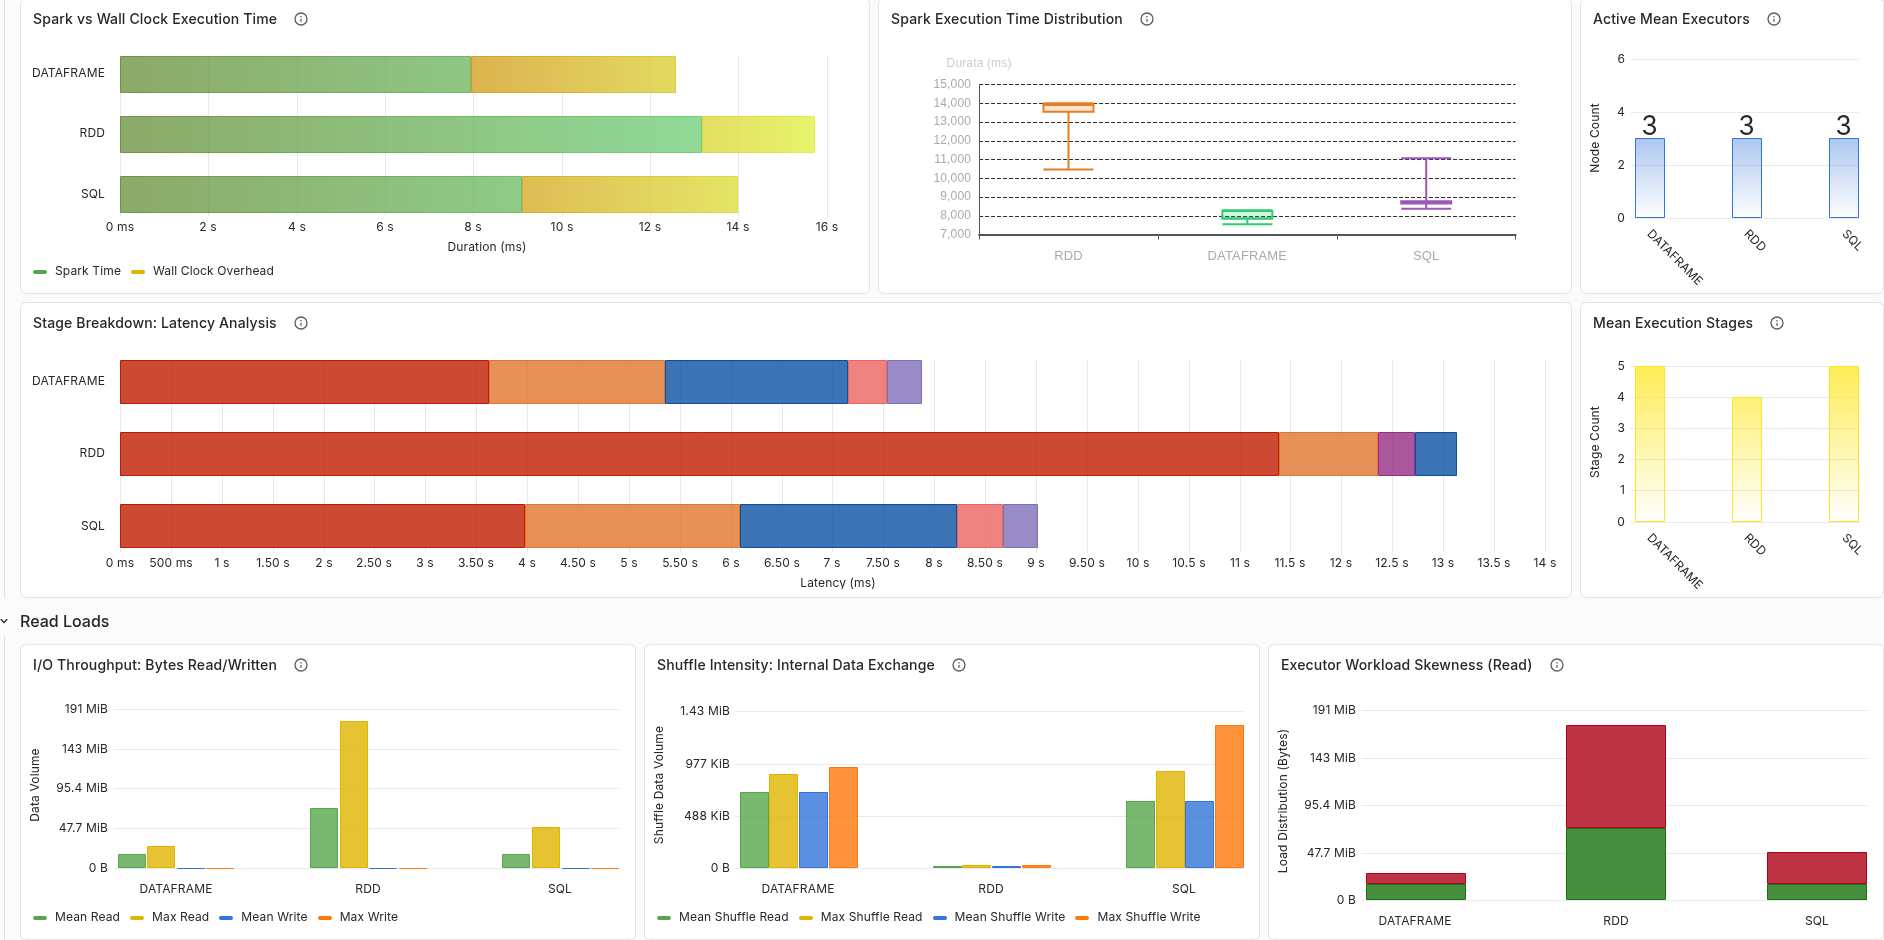
\includegraphics[width=1\textwidth]{../Results/charts/telemetry/emr/part_prun/metrics_emr_hourly_delay_percentiles_tdigest_part_prun_cropped}

    \vspace{1cm}

    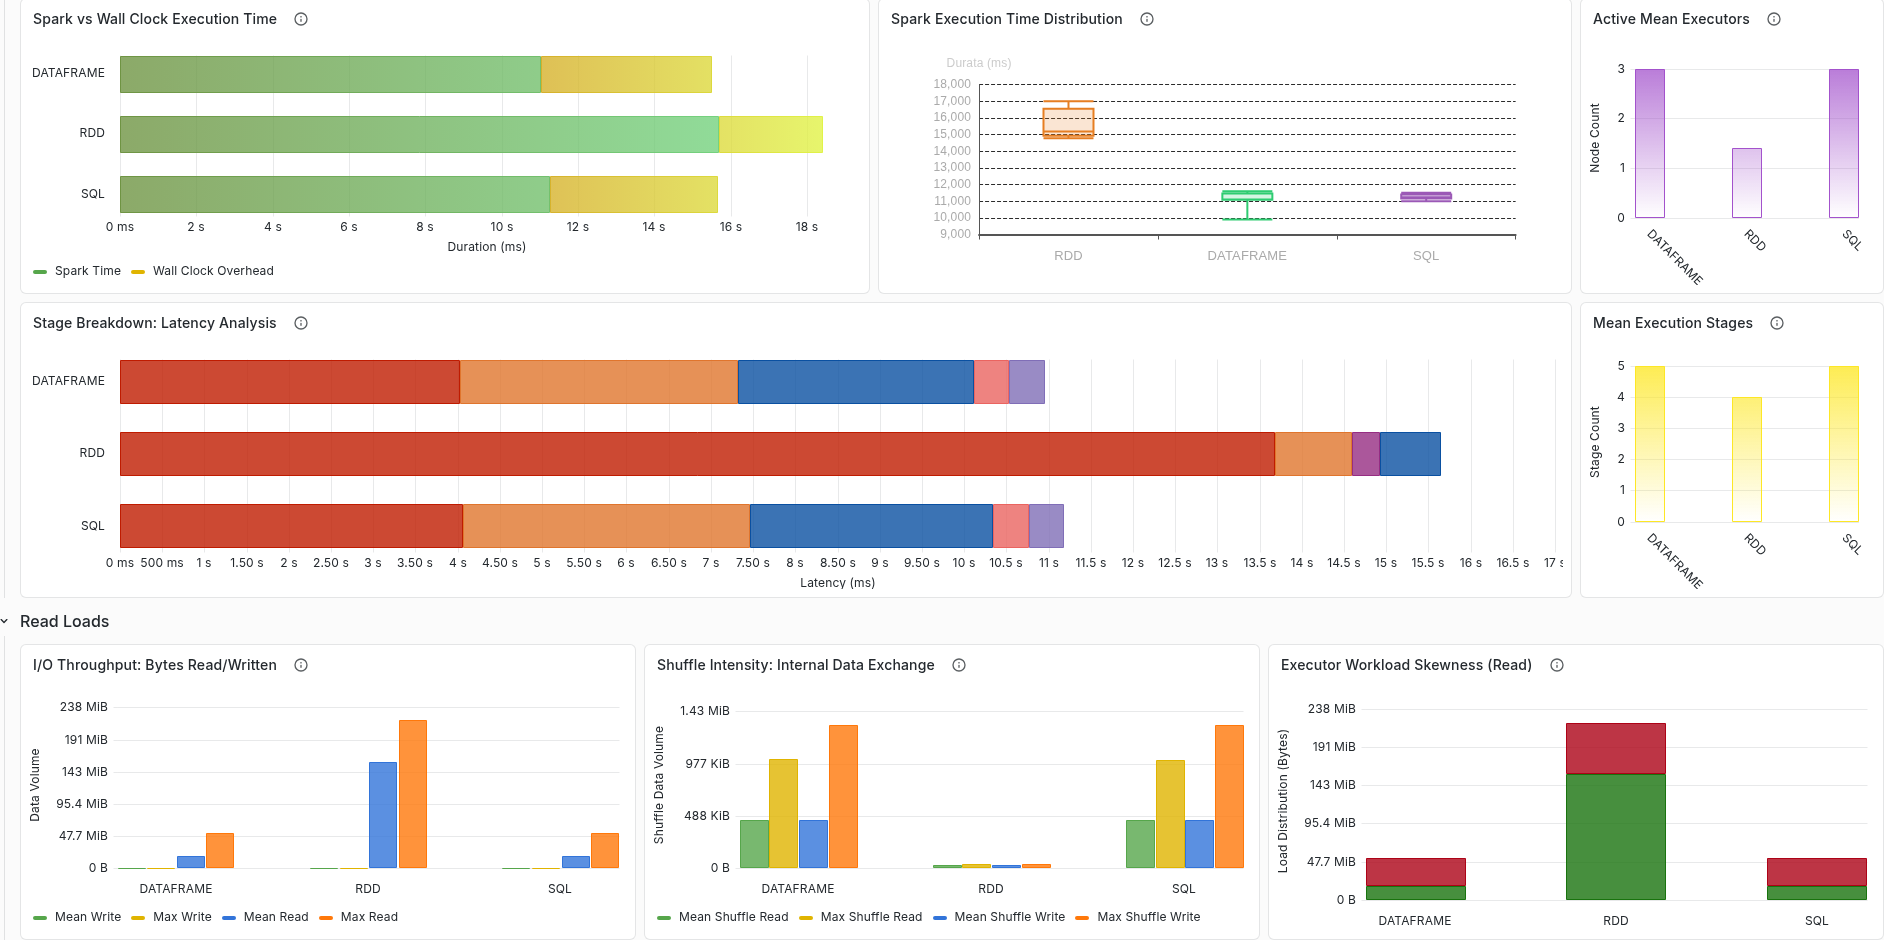
\includegraphics[width=1\textwidth]{../Results/charts/telemetry/emr/pred_push/metrics_emr_hourly_delay_percentiles_tdigest_pred_push_cropped}
    \caption{Telemetria Query 3 su AWS EMR con algoritmo T-Digest: Partition Pruning (sopra) vs Predicate Pushdown (sotto).}
    \label{fig:telemetry_q3_tdigest_emr}
\end{figure}

\clearpage

\subsection{Query 4: Clustering delle Compagnie}

\begin{figure}[!htbp]
    \centering
    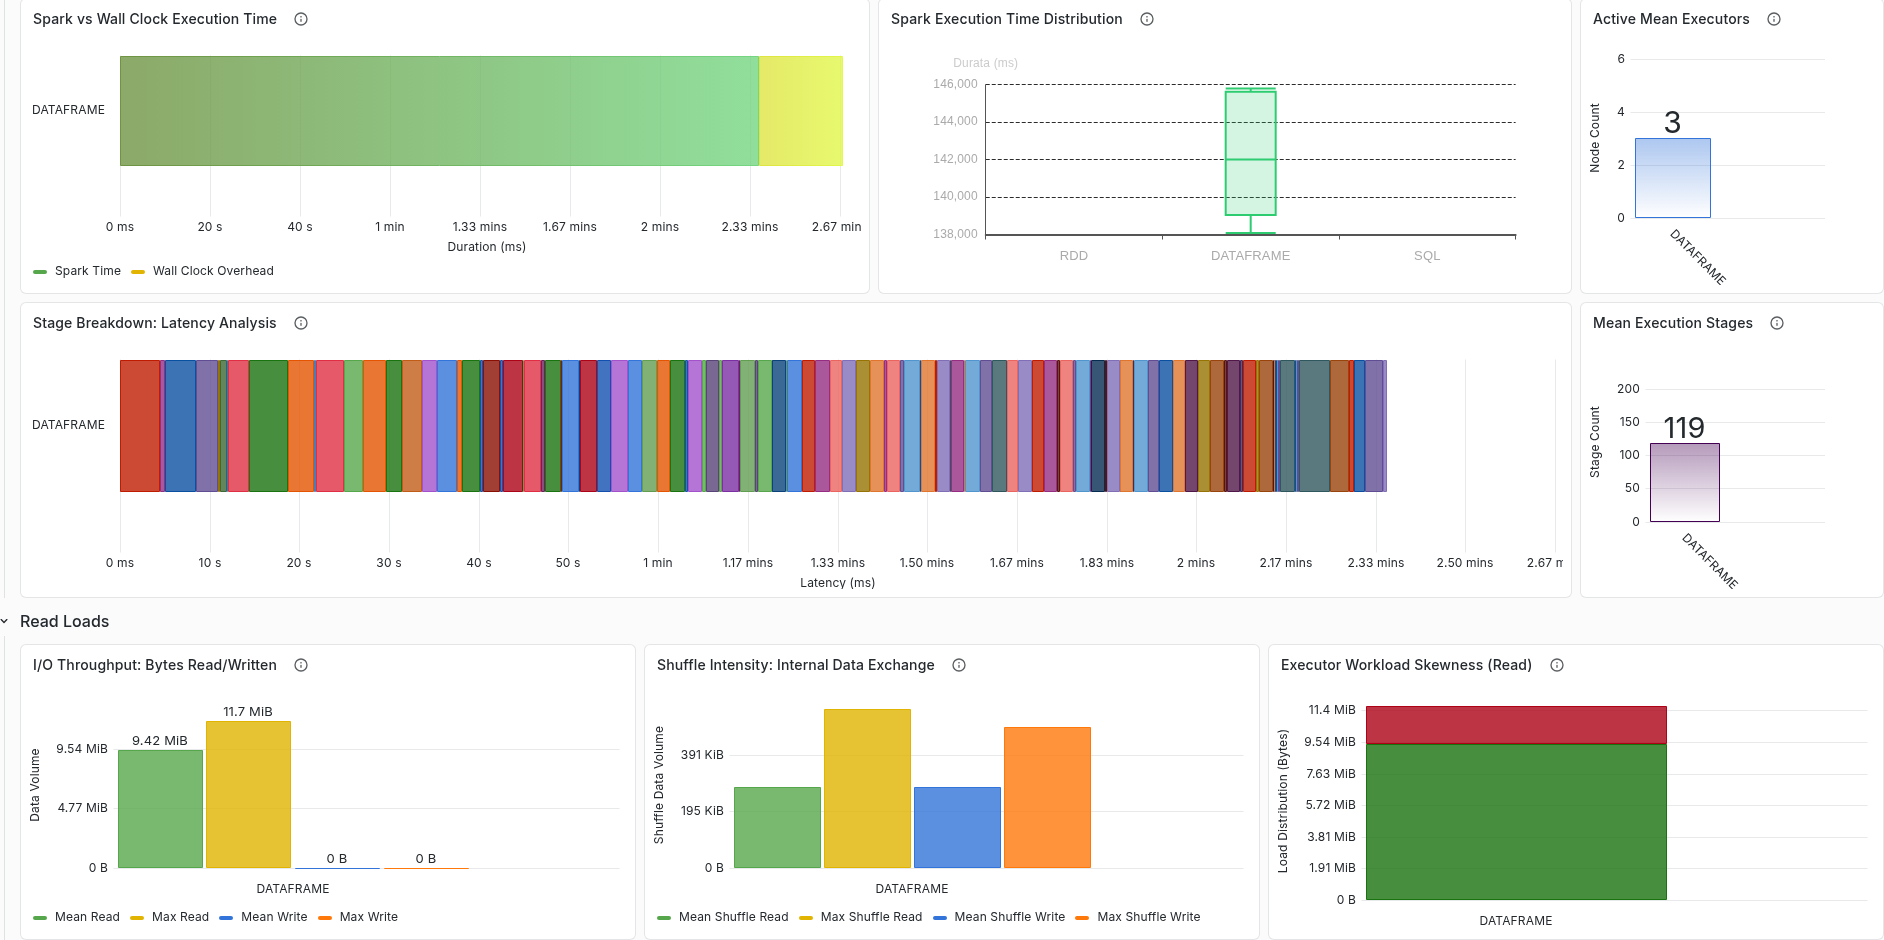
\includegraphics[width=1\textwidth]{../Results/charts/telemetry/ec2/part_prun/metrics_ec2_airline_clustering_part_prun_cropped}

    \vspace{1cm}

    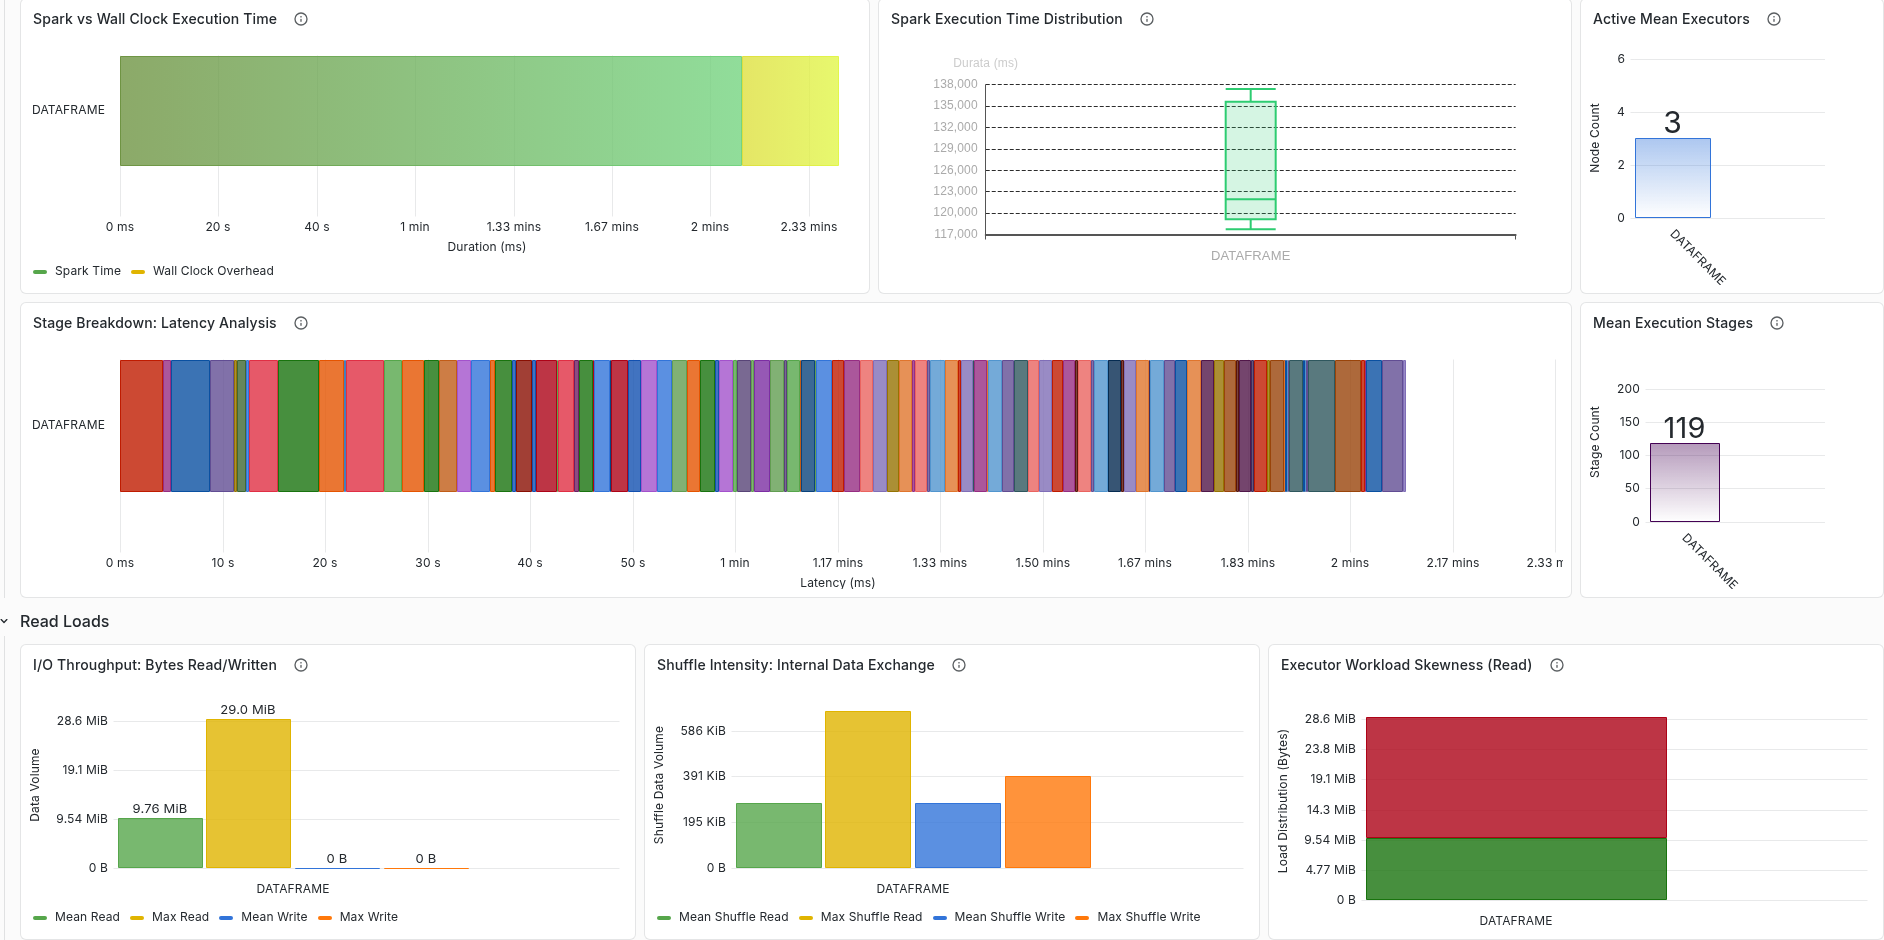
\includegraphics[width=1\textwidth]{../Results/charts/telemetry/ec2/pred_push/metrics_ec2_airline_clustering_pred_push_cropped}
    \caption{Telemetria Query 4 su AWS EC2: Partition Pruning (sopra) vs Predicate Pushdown (sotto).}
    \label{fig:telemetry_q4_ec2}
\end{figure}

\clearpage

\begin{figure}[!htbp]
    \centering
    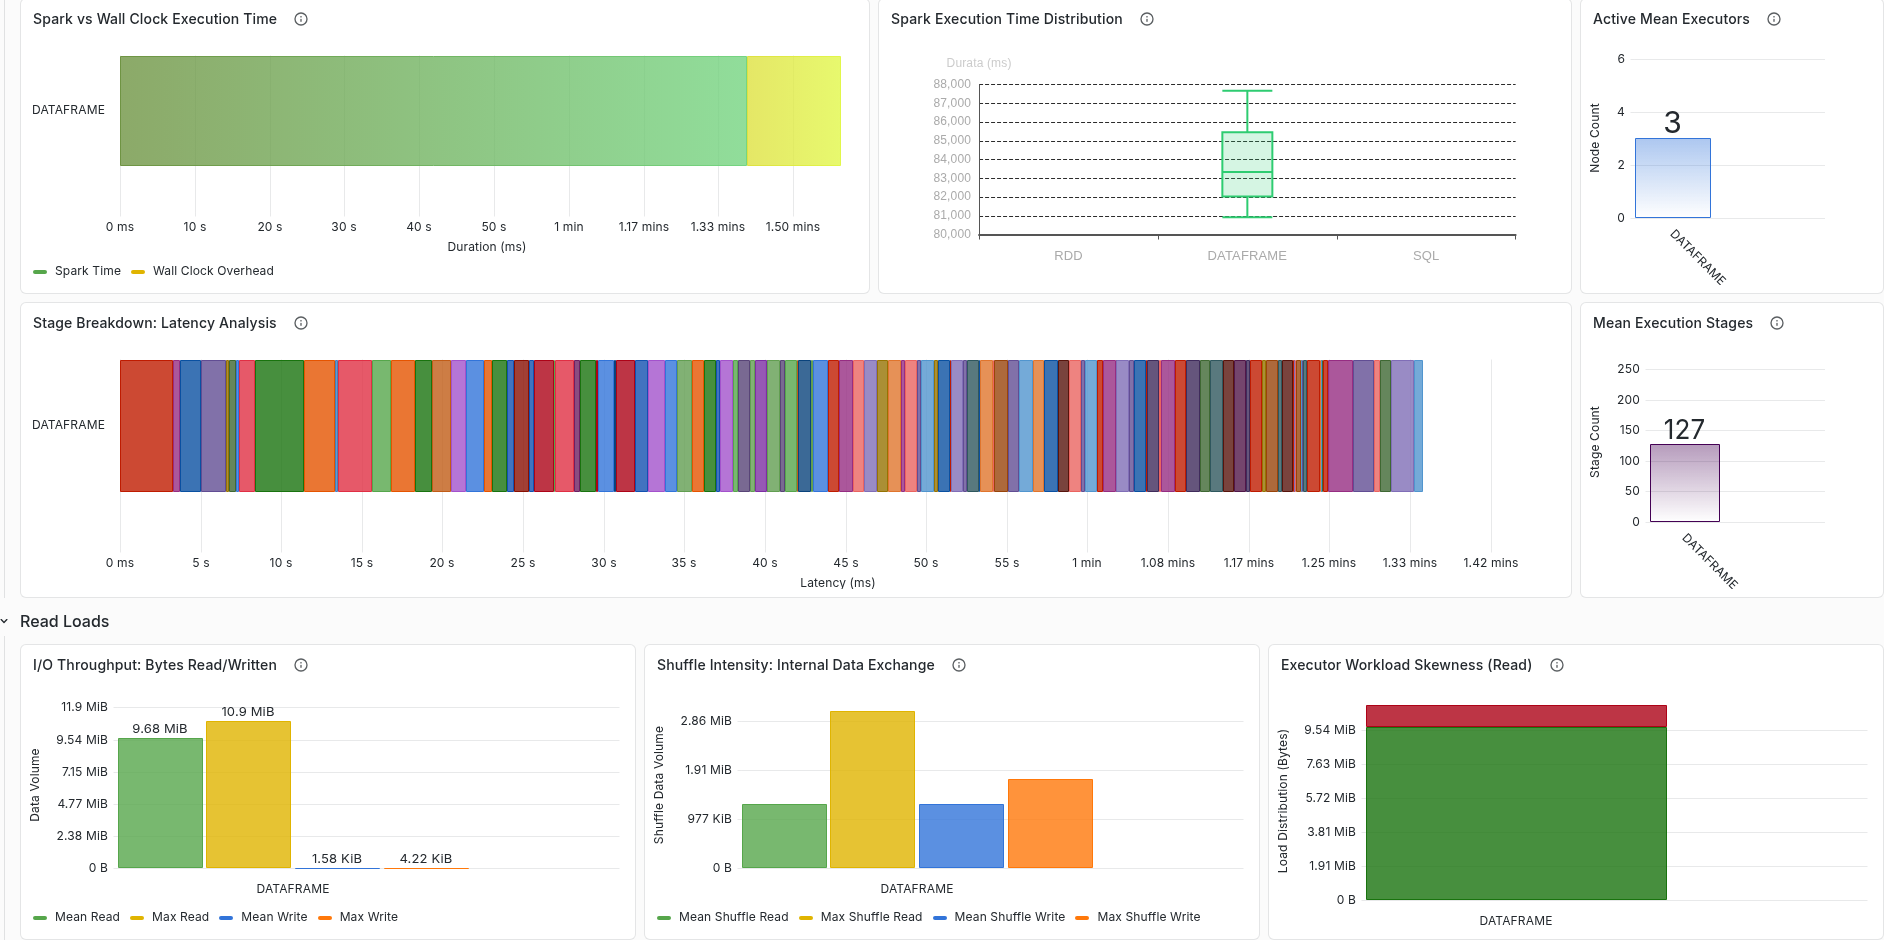
\includegraphics[width=1\textwidth]{../Results/charts/telemetry/emr/part_prun/metrics_emr_airline_clustering_part_prun_cropped}

    \vspace{1cm}

    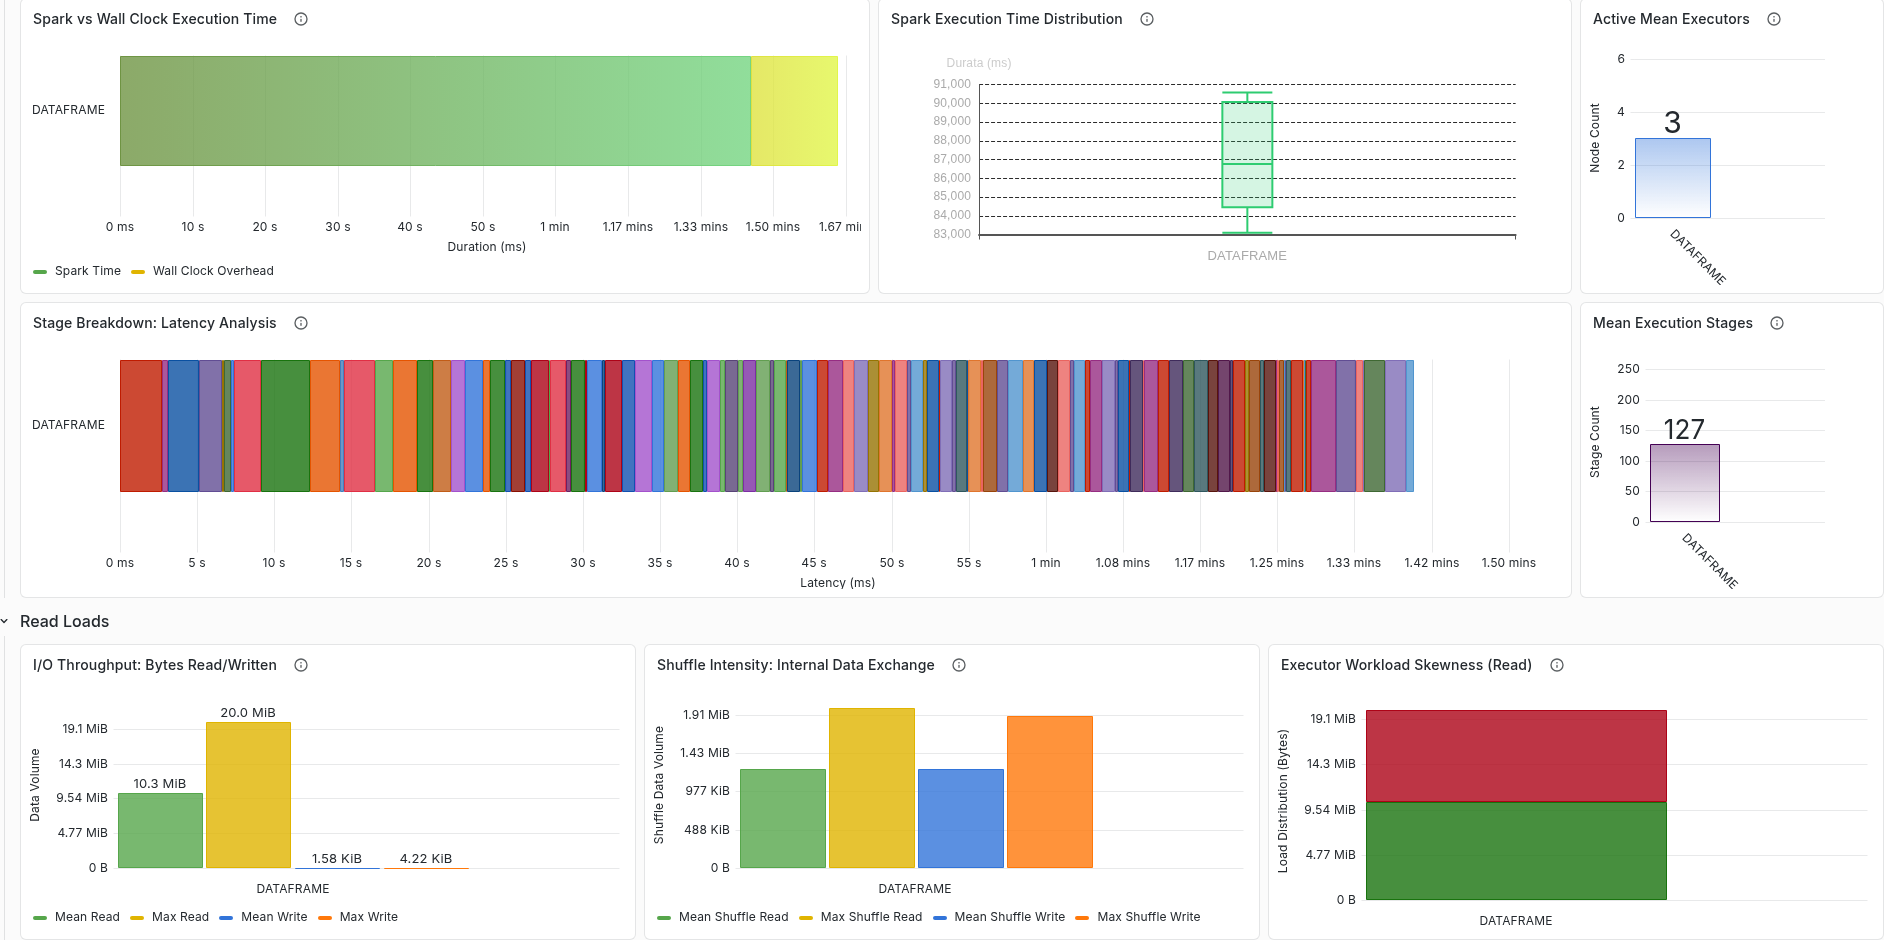
\includegraphics[width=1\textwidth]{../Results/charts/telemetry/emr/pred_push/metrics_emr_airline_clustering_pred_push_cropped}
    \caption{Telemetria Query 4 su AWS EMR: Partition Pruning (sopra) vs Predicate Pushdown (sotto).}
    \label{fig:telemetry_q4_emr}
\end{figure}

\clearpage

\section{Risultati Analitici delle Query}\label{sec:appendix_results}
In questa appendice vengono riportati in dettaglio i risultati analitici ottenuti dall'applicazione della pipeline SAE.

\subsection{Query 1}\label{subsec:results_q1}
Per la Query 1, vengono presentati i risultati relativi al trend dei ritardi medi mensili e al tasso di cancellazione per le compagnie aeree in esame.

\begin{figure}[!htbp]
    \centering
    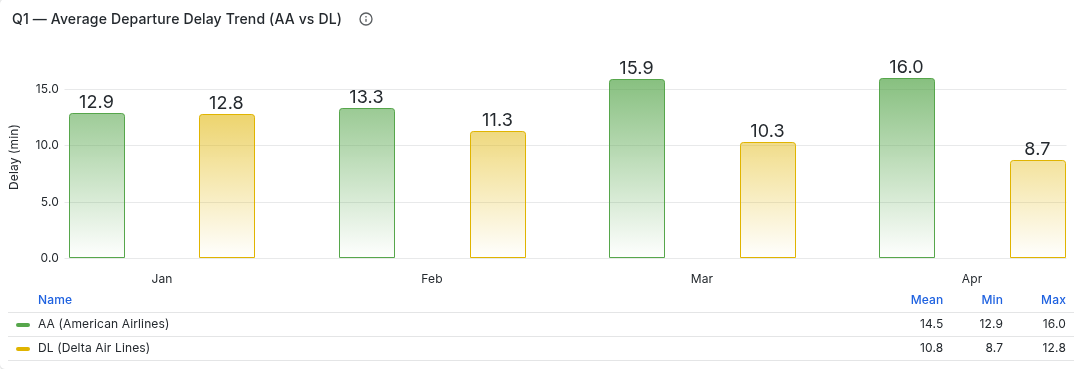
\includegraphics[width=1\textwidth]{../Results/charts/result/Q1_average_delay_trend}
    \caption{Risultati Query 1: Trend dei ritardi medi mensili.}
    \label{fig:results_q1_average_delay_trend}
\end{figure}

\begin{figure}[!htbp]
    \centering
    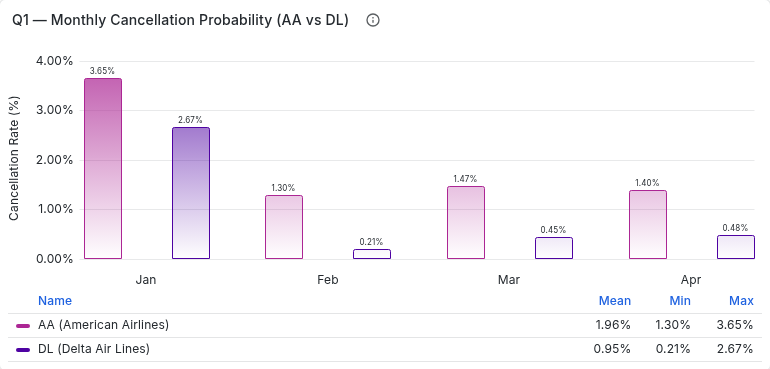
\includegraphics[width=1\textwidth]{../Results/charts/result/Q1_cancellation_rate_probabilty}
    \caption{Risultati Query 1: Tasso e probabilità di cancellazione.}
    \label{fig:results_q1_cancellation_rate_probability}
\end{figure}

\clearpage

\subsection{Query 2}\label{subsec:results_q2}
Nella Query 2, vengono presentati i risultati relativi alla classifica delle tratte con i ritardi medi più elevati e la composizione percentuale delle cause di ritardo.

\begin{figure}[!htbp]
    \centering
    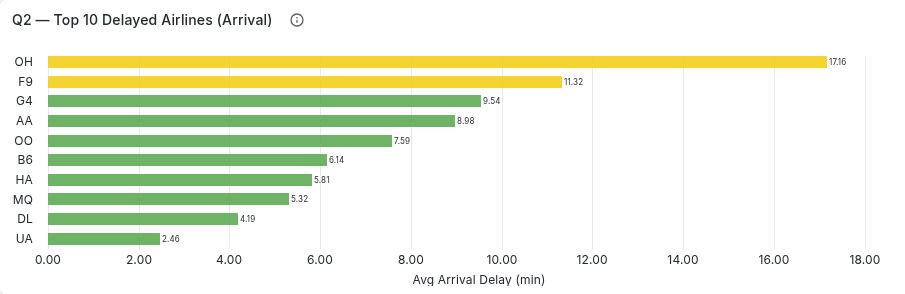
\includegraphics[width=1\textwidth]{../Results/charts/result/Q2_top10_arrival_delay}
    \caption{Risultati Query 2: Classifica delle 10 tratte con i ritardi medi più elevati.}
    \label{fig:results_q2_top10_arrival_delay}
\end{figure}

\begin{figure}[!htbp]
    \centering
    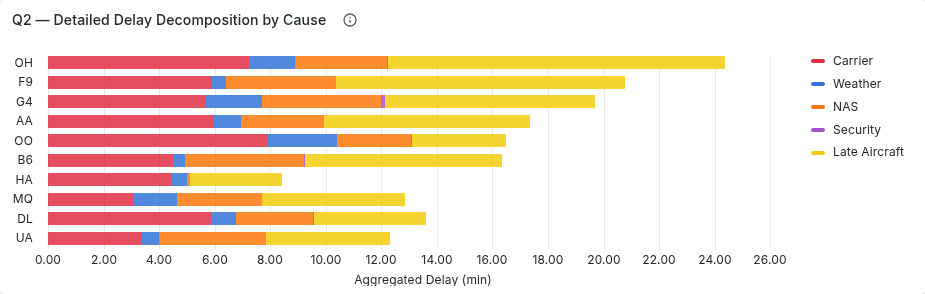
\includegraphics[width=1\textwidth]{../Results/charts/result/Q2_delay_composition}
    \caption{Risultati Query 2: Decomposizione percentuale delle cause di ritardo.}
    \label{fig:results_q2_delay_composition}
\end{figure}

\clearpage

\subsection{Query 3}\label{subsec:results_q3}
Per la Query 3, vengono presentati, per le quattro compagnie aeree in esame, la distribuzione mediana oraria e il trend dei percentili critici stimati.

\begin{figure}[!htbp]
    \centering
    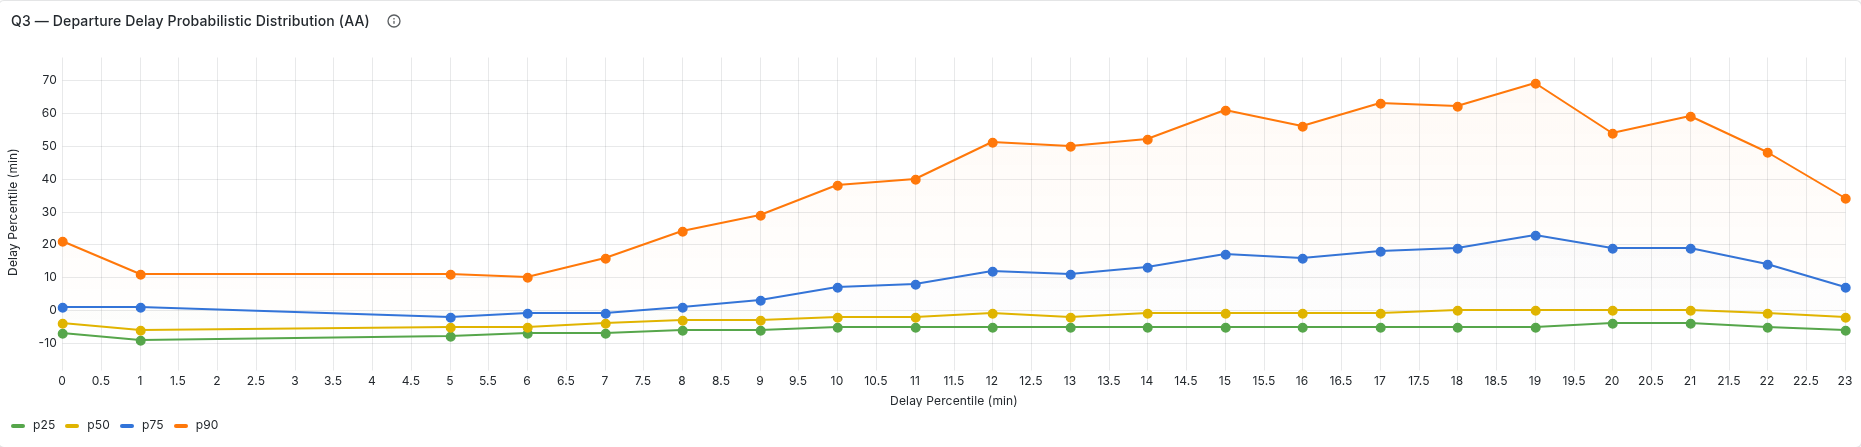
\includegraphics[width=0.93\textwidth]{../Results/charts/result/Q3_percentiles_trend_AA}
    \caption{Risultati Query 3 (AA): Trend orario dei percentili di ritardo critici.}
    \label{fig:results_q3_percentiles_trend_AA}
\end{figure}

\begin{figure}[!htbp]
    \centering
    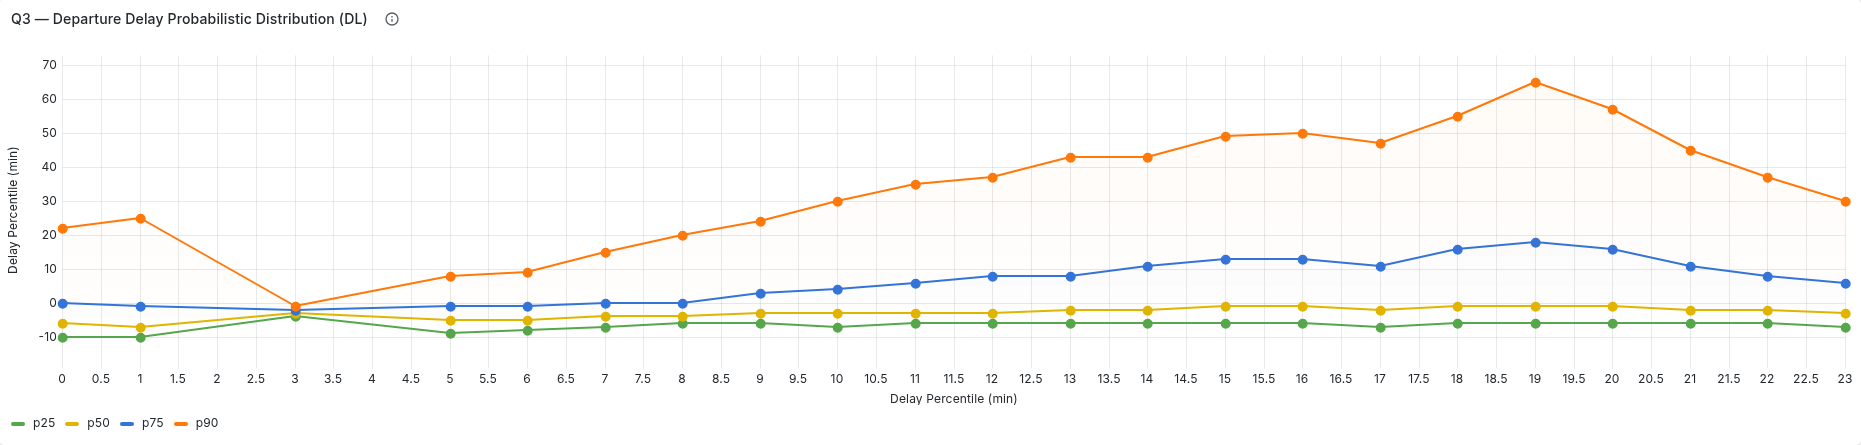
\includegraphics[width=0.93\textwidth]{../Results/charts/result/Q3_percentiles_trend_DL}
    \caption{Risultati Query 3 (DL): Trend orario dei percentili di ritardo critici.}
    \label{fig:results_q3_percentiles_trend_DL}
\end{figure}

\begin{figure}[!htbp]
    \centering
    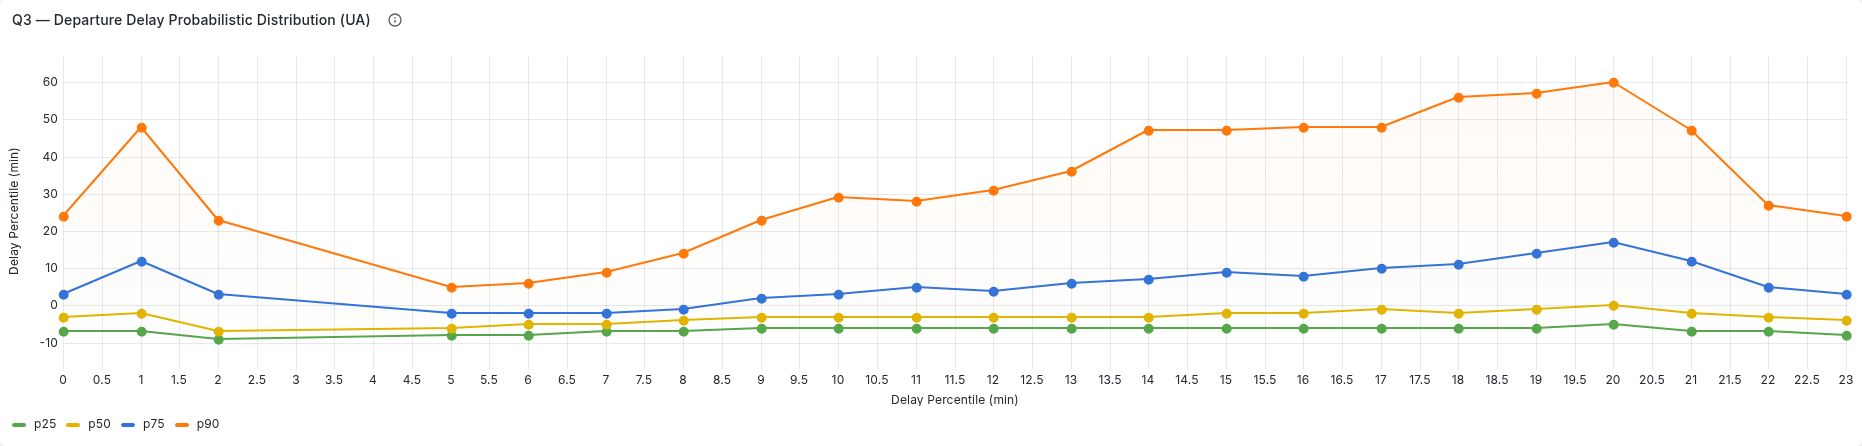
\includegraphics[width=0.93\textwidth]{../Results/charts/result/Q3_percentiles_trend_UA}
    \caption{Risultati Query 3 (UA): Trend orario dei percentili di ritardo critici.}
    \label{fig:results_q3_percentiles_trend_UA}
\end{figure}

\begin{figure}[!htbp]
    \centering
    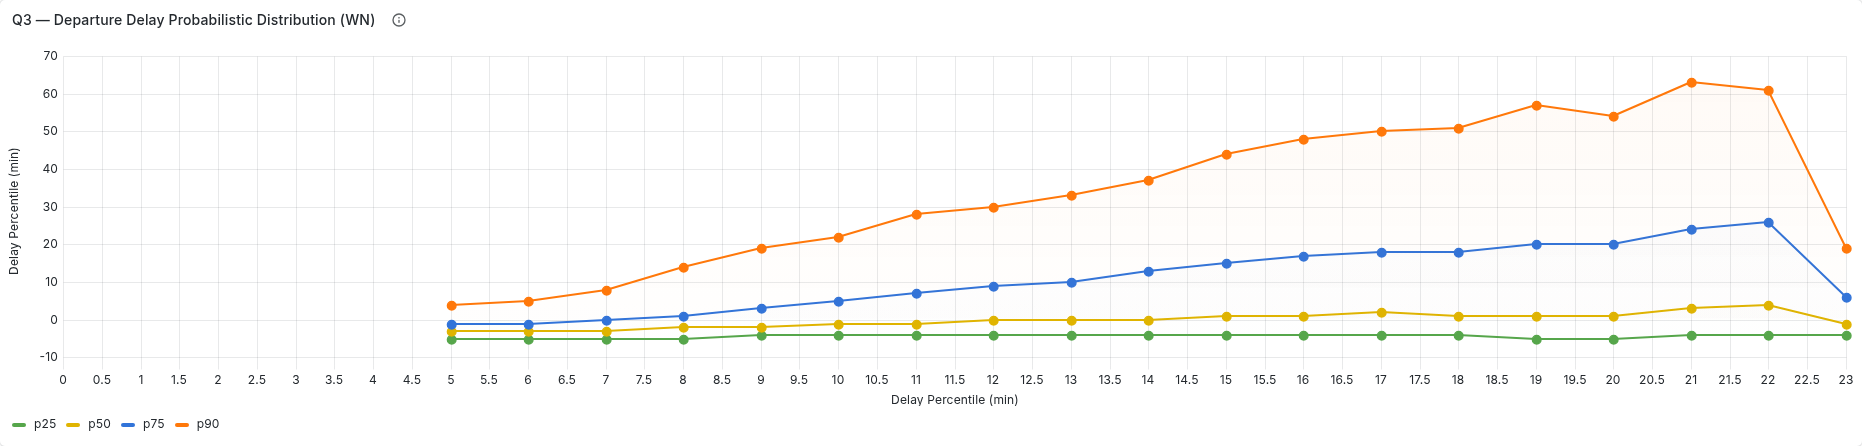
\includegraphics[width=0.93\textwidth]{../Results/charts/result/Q3_percentiles_trend_WN}
    \caption{Risultati Query 3 (WN): Trend orario dei percentili di ritardo critici.}
    \label{fig:results_q3_percentiles_trend_WN}
\end{figure}

\clearpage

\begin{figure}[!htbp]
    \centering
    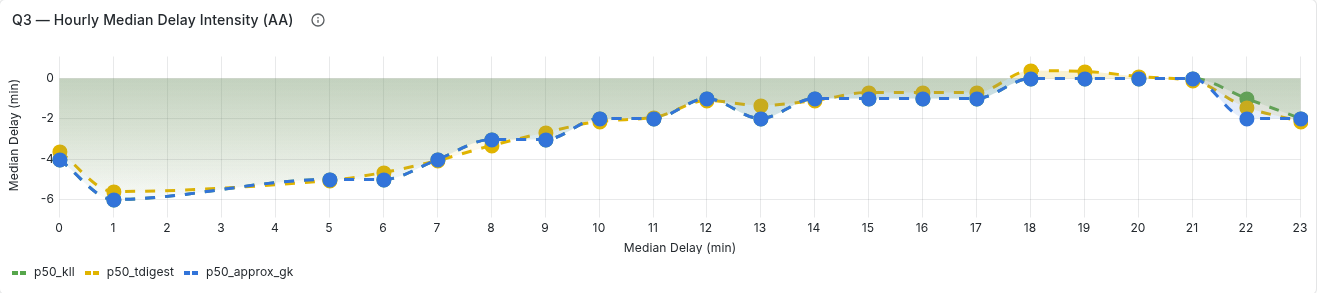
\includegraphics[width=0.85\textwidth]{../Results/charts/result/Q3_median_distribution_detail_AA}
    \caption{Risultati Query 3 (AA): Distribuzione oraria del ritardo mediano.}
    \label{fig:results_Q3_median_distribution_detail_AA}
\end{figure}

\begin{figure}[!htbp]
    \centering
    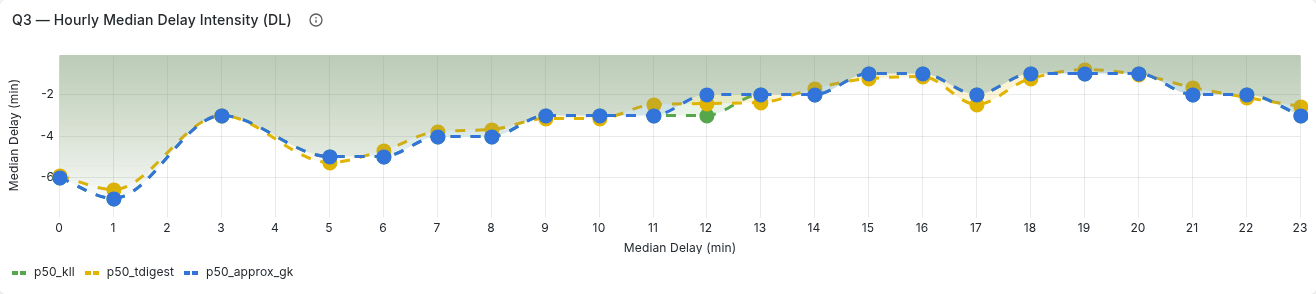
\includegraphics[width=0.85\textwidth]{../Results/charts/result/Q3_median_distribution_detail_DL}
    \caption{Risultati Query 3 (DL): Distribuzione oraria del ritardo mediano.}
    \label{fig:results_Q3_median_distribution_detail_DL}
\end{figure}

\begin{figure}[!htbp]
    \centering
    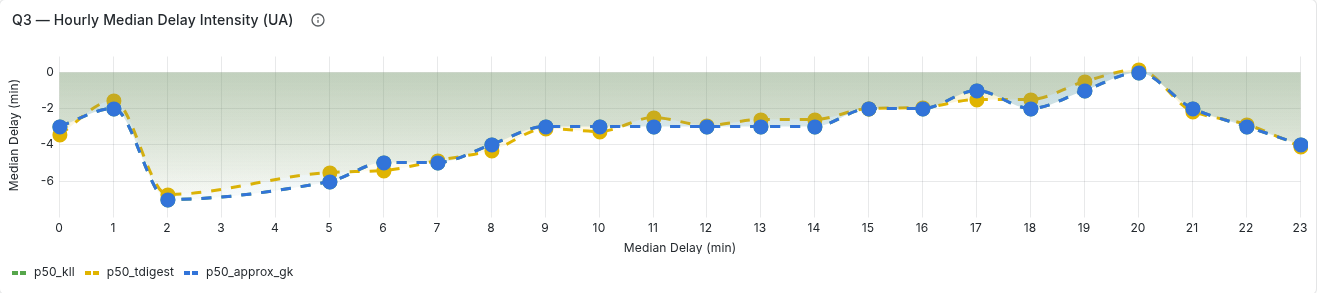
\includegraphics[width=0.85\textwidth]{../Results/charts/result/Q3_median_distribution_detail_UA}
    \caption{Risultati Query 3 (UA): Distribuzione oraria del ritardo mediano.}
    \label{fig:results_Q3_median_distribution_detail_UA}
\end{figure}

\begin{figure}[!htbp]
    \centering
    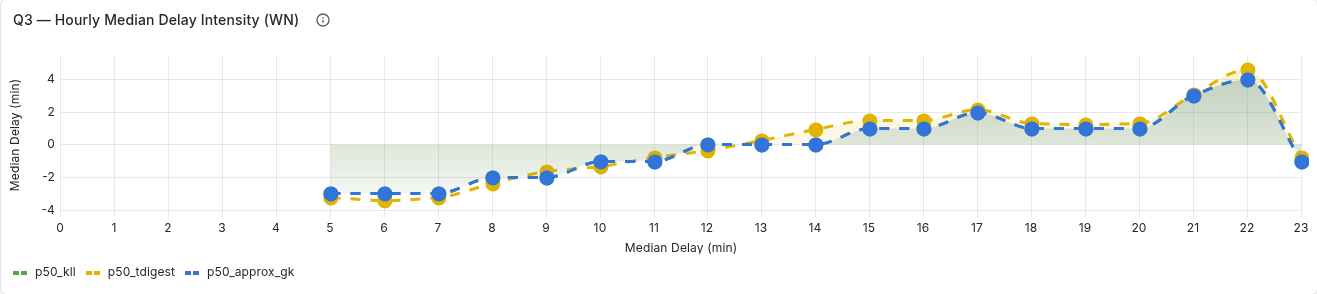
\includegraphics[width=0.85\textwidth]{../Results/charts/result/Q3_median_distribution_detail_WN}
    \caption{Risultati Query 3 (WN): Distribuzione oraria del ritardo mediano.}
    \label{fig:results_Q3_median_distribution_detail_WN}
\end{figure}

\begin{figure}[!htbp]
    \centering
    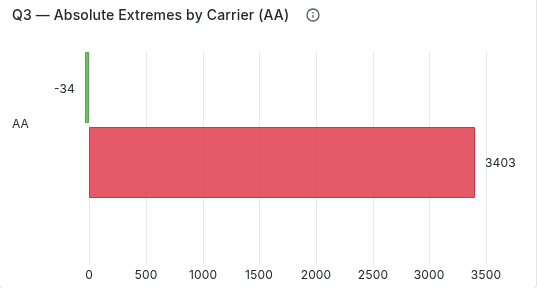
\includegraphics[width=0.22\textwidth]{../Results/charts/result/Q3_median_distribution_min_max_AA}
    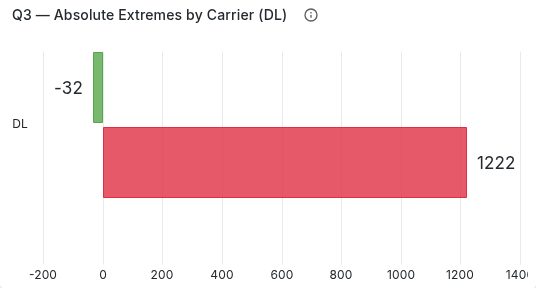
\includegraphics[width=0.22\textwidth]{../Results/charts/result/Q3_median_distribution_min_max_DL}
    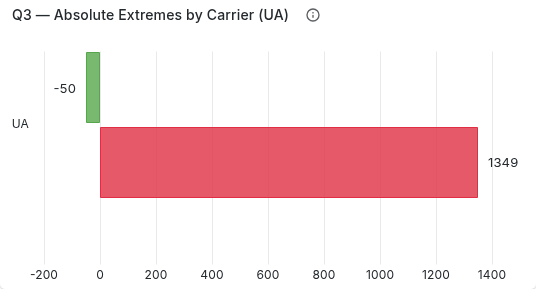
\includegraphics[width=0.22\textwidth]{../Results/charts/result/Q3_median_distribution_min_max_UA}
    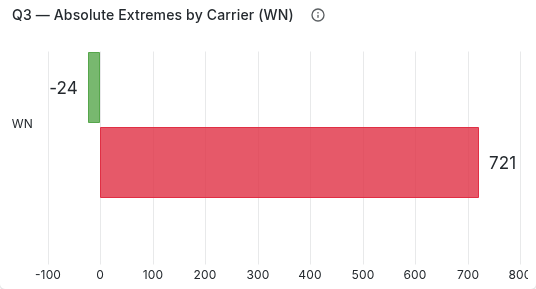
\includegraphics[width=0.22\textwidth]{../Results/charts/result/Q3_median_distribution_min_max_WN}
    \caption{Risultati Query 3: Valori estremi dei ritardi per American Airlines (AA), Delta Air Lines (DL), United Airlines (UA) e Southwest Airlines (WN) (da sinistra a destra).}
    \label{fig:results_q3_min_max}
\end{figure}

\clearpage

\subsection{Query 4}\label{subsec:results_q4}
Per la Query 4, vengono presentati i risultati relativi alla distribuzione geometrica dei cluster identificati tramite PCA, i valori medi delle feature per ciascun cluster e la classificazione granulare dei vettori.

\begin{figure}[!htbp]
    \centering
    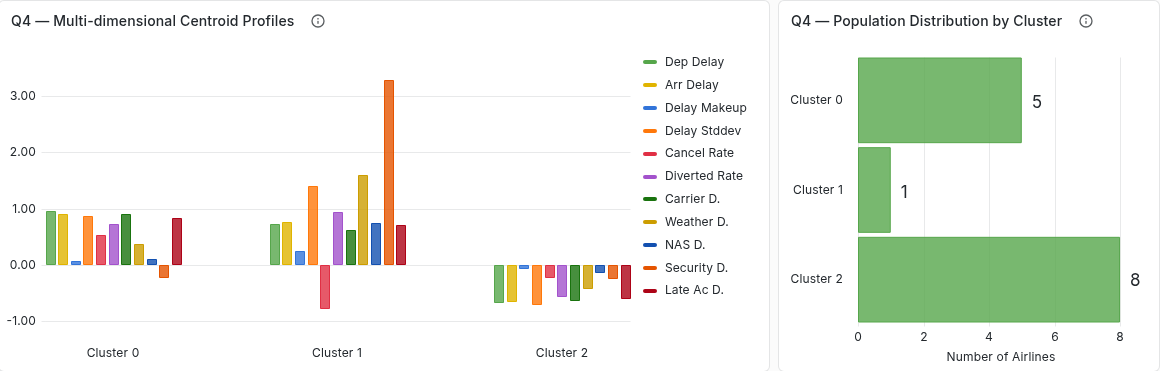
\includegraphics[width=0.70\textwidth]{../Results/charts/result/Q4_cluster_center}
    \caption{Valori medi delle feature per ciascun cluster identificato nella Query 4. Le barre rappresentano le medie normalizzate delle singole features per permettere un confronto relativo tra i cluster.}
    \label{fig:results_q4_cluster_center}
\end{figure}

\begin{figure}[!htbp]
    \centering
    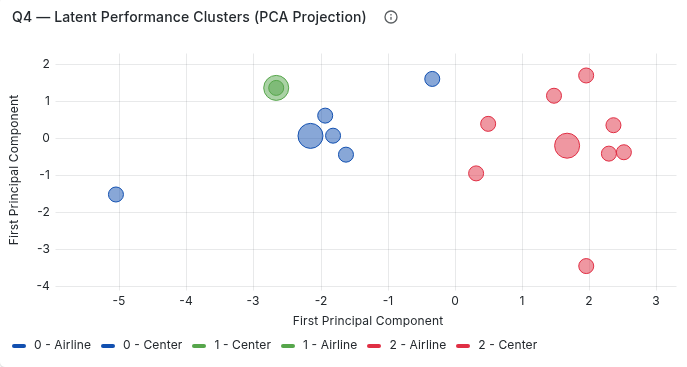
\includegraphics[width=0.45\textwidth]{../Results/charts/result/Q4_cluster_distribution}
    \caption{Risultati Query 4: Distribuzione geometrica dei cluster estratti tramite PCA.}
    \label{fig:results_q4_cluster_distribution}
\end{figure}

\begin{table}[!htbp]
    \centering
    \footnotesize\sffamily
    \caption{Risultati Query 4: Metriche operative medie (valori grezzi) e classificazione.}
    \begin{tabular*}{\textwidth}{@{\extracolsep{\fill}}l|ccccccc|ccccc@{}}
        \toprule
        \textbf{ID} & \textbf{Dep.} & \textbf{Arr.} & \textbf{Makeup} & \textbf{StdDev} & \textbf{Div.\%} & \textbf{Can.\%} & \textbf{Clus.} & \textbf{Carr.} & \textbf{Weat.} & \textbf{NAS} & \textbf{Secu.} & \textbf{Late Air.} \\
        \midrule
        \texttt{UA} & 9.03 & 2.46 & -6.52 & 47.56 & 0.21 & 0.69 & 2 & 3.36 & 0.61 & 3.80 & 0.00 & 4.44 \\
        \texttt{NK} & 9.17 & 2.39 & -6.77 & 48.28 & 0.13 & 1.41 & 2 & 3.13 & 0.28 & 6.13 & 0.03 & 3.04 \\
        \texttt{DL} & 10.71 & 4.19 & -6.40 & 55.11 & 0.19 & 0.94 & 2 & 5.80 & 0.88 & 2.76 & 0.01 & 4.01 \\
        \texttt{MQ} & 8.44 & 5.32 & -3.12 & 50.71 & 0.20 & 2.82 & 2 & 3.00 & 1.50 & 2.97 & 0.02 & 4.99 \\
        \texttt{HA} & 6.35 & 5.81 & -0.52 & 37.42 & 0.10 & 1.21 & 2 & 4.41 & 0.53 & 0.09 & 0.02 & 3.24 \\
        \texttt{YX} & 4.78 & 0.69 & -4.04 & 42.22 & 0.16 & 2.26 & 2 & 2.82 & 0.53 & 3.67 & 0.01 & 3.39 \\
        \texttt{AS} & 5.52 & 1.30 & -4.22 & 36.08 & 0.16 & 1.00 & 2 & 2.75 & 0.44 & 2.74 & 0.04 & 3.59 \\
        \texttt{WN} & 9.35 & 1.76 & -7.58 & 35.25 & 0.16 & 1.14 & 2 & 2.58 & 0.27 & 1.94 & 0.02 & 4.78 \\
        \midrule
        \texttt{AA} & 14.59 & 8.98 & -5.59 & 74.97 & 0.25 & 1.94 & 0 & 5.82 & 0.99 & 2.90 & 0.02 & 7.24 \\
        \texttt{B6} & 12.51 & 6.14 & -6.33 & 56.11 & 0.25 & 1.23 & 0 & 4.43 & 0.43 & 4.24 & 0.03 & 6.98 \\
        \texttt{OO} & 11.68 & 7.59 & -4.04 & 62.92 & 0.24 & 1.47 & 0 & 7.80 & 2.43 & 2.63 & 0.02 & 3.32 \\
        \texttt{F9} & 16.00 & 11.32 & -4.62 & 71.65 & 0.16 & 1.67 & 0 & 5.82 & 0.48 & 3.87 & 0.00 & 10.22 \\
        \texttt{OH} & 19.78 & 17.16 & -2.60 & 82.75 & 0.21 & 6.09 & 0 & 6.79 & 1.56 & 3.10 & 0.03 & 11.37 \\
        \midrule
        \texttt{G4} & 13.87 & 9.54 & -4.31 & 78.39 & 0.23 & 0.66 & 1 & 5.63 & 2.02 & 4.23 & 0.15 & 7.47 \\
        \bottomrule
    \end{tabular*}
    \label{tab:results_q4_metrics}
\end{table}

\centering
\textbf{Legenda:}\\
Dep./Arr.: ritardo medio partenza/arrivo;
\\Makeup: capacità di recupero ritardo in volo;
\\StdDev: deviazione standard ritardo arrivo;
\\Div.\%/Can.\%: tasso deviazioni e cancellazioni;
\\Clus.: ID Cluster;
\\Carr./Weat./NAS/Secu./Late Air.: cause di ritardo medie in minuti;

\end{document}
